%!TEX root = ../Thesis.tex
%% Basierend auf TeXnicCenter-Vorlage von Mark Müller
%%                      Willi Nüßer
%%                      Waldemar Penner     
%%                      Ulrich Reus
%%                      Frank Plass
%%                      Oliver Tribeß 
%%                      Daniel Hintze     
%%%%%%%%%%%%%%%%%%%%%%%%%%%%%%%%%%%%%%%%%%%%%%%%%%%%%%%%%%%%%%%%%%%%%%%

% Wählen Sie die Optionen aus, indem Sie % vor der Option entfernen  
% Dokumentation des KOMA-Script-Packets: scrguide

%%%%%%%%%%%%%%%%%%%%%%%%%%%%%%%%%%%%%%%%%%%%%%%%%%%%%%%%%%%%%%%%%%%%%%%
%% Optionen zum Layout des Artikels                                  %%
%%%%%%%%%%%%%%%%%%%%%%%%%%%%%%%%%%%%%%%%%%%%%%%%%%%%%%%%%%%%%%%%%%%%%%%
\documentclass[%
paper=A4,         % alle weiteren Papierformat einstellbar
fontsize=12pt,    % Schriftgröße (12pt, 11pt (Standard))
BCOR12mm,         % Bindekorrektur, bspw. 1 cm
DIV14,            % breiter Satzspiegel
parskip=half*,    % Absatzformatierung s. scrguide 3.1
headsepline,      % Trennline zum Seitenkopf  
%footsepline,     % Trennline zum Seitenfuß
%normalheadings,  % Überschriften etwas kleiner (smallheadings)
listof=totoc,     % Tabellen & Abbildungsverzeichnis ins Inhaltsverzeichnis      
%bibtotoc,        % Literaturverzeichnis im Inhalt 
%draft            % Überlangen Zeilen in Ausgabe gekennzeichnet
footinclude=false,% Fußzeile in die Satzspiegelberechnung einbeziehen 
headinclude=true, % Kopfzeile in die Satzspiegelberechnung einbeziehen 
final             % draft beschleunigt die Kompilierung
]
{scrartcl}

%\setuptoc{toc}{totoc} % Inhaltsverzeichnis ins Inhaltsverzeichnis

% Neue Deutsche Rechtschreibung und Deutsche Standardtexte
\usepackage[ngerman]{babel} 

% Umlaute können verwendet werden
\usepackage[utf8]{inputenc}   

% Echte Umlaute
\usepackage[T1]{fontenc} 

% Latin Modern Font, Type1-Schriftart für nicht-englische Texte
\usepackage{lmodern} 

% 1/2-zeiliger Zeilenabstand
\usepackage[onehalfspacing]{setspace}

% Für die Defenition eigener Kopf- und Fußzeilen
\usepackage{fancyhdr} 

% Für die Verwendung von Grafiken
\usepackage[pdftex]{graphicx}

% Bessere Tabellen
\usepackage{tabularx}

% Für die Befehle \toprule, \midrule und \bottomrule, z.B. in Tabellen 
\usepackage{booktabs}

% Erlaubt die Benutzung von Farben
\usepackage{color}

% Verbessertes URL-Handling mit \url{http://...}
\usepackage{url}

% Listen ohne Abstände \begin{compactlist}...\end{compactlist}
\usepackage{paralist} 

% Ausgabe der aktuellen Uhrzeit für die Draft-Versionen
\usepackage{datetime}

% Multirow zur Zentrierung von Inhalt in einer Tabellenzelle
\usepackage{multirow}

% to use multi row header
\usepackage{makecell}

% Deutsche Anführungszeichen
\usepackage[babel,german=quotes]{csquotes}

% Konfiguration der Abbildungs- und Tabellenbezeichnungen
\usepackage[format=hang, font={footnotesize, sf}, labelfont=bf, justification=raggedright,singlelinecheck=false]{caption}

% Verbessert die Lesbarkeit durch Mikrotypografie
\usepackage[activate={true,nocompatibility},final,tracking=true,kerning=true,spacing=true,factor=1100,stretch=10,shrink=10]{microtype}  

% Zitate und Quellenverzeichnis
\usepackage[
    bibstyle=authoryear,
    citestyle=authoryear-fhdw,  
    firstinits=false,         % false = Vornamen werden ausgeschrieben
    natbib=true,
    urldate=long,             % "besucht am" - Datum
    %url=false,
    date=long,                
    dashed=false, 
    maxcitenames=3,           % max. Anzahl Autorennamen in Zitaten
    maxbibnames=99,           % max. Anzahl Autorennamen im Quellenverzeichnis
    %backend=bibtex           % Ggf. für ältere Distributionen bibtex verwenden
    backend=biber
]{biblatex}
  
% Bibliograpthy
\bibliography{library/library}

% Keine Einrückung bei einem neuen Absatz 
\parindent 0pt 

% Ebenentiefe der Nummerierung
\setcounter{secnumdepth}{3}

% Gliederungstiefe im Inhaltsverzeichnis 
\setcounter{tocdepth}{3} 

% Tabellen- und Abbildungsverzeichnis mit Bezeichnung:
\usepackage[titles]{tocloft}

% Formeln
\usepackage{amsmath}

% Sourcecode-Listings
\usepackage{listings}

% Bestimmte Warnungen unterdrücken
% siehe http://tex.stackexchange.com/questions/51867/koma-warning-about-toc
\usepackage{scrhack} 

%% http://tex.stackexchange.com/questions/126839/how-to-add-a-colon-after-listing-label
\makeatletter
\begingroup\let\newcounter\@gobble\let\setcounter\@gobbletwo
  \globaldefs\@ne \let\c@loldepth\@ne
  \newlistof{listings}{lol}{\lstlistlistingname}
\endgroup
\let\l@lstlisting\l@listings
\makeatother

\renewcommand*\cftfigpresnum{Abbildung~}
\renewcommand*\cfttabpresnum{Tabelle~}
\renewcommand*\cftlistingspresnum{Listing~}
\renewcommand{\cftfigaftersnum}{:}
\renewcommand{\cfttabaftersnum}{:}
\renewcommand{\cftlistingsaftersnum}{:}
\settowidth{\cftfignumwidth}{\cftfigpresnum 99~\cftfigaftersnum}
\settowidth{\cfttabnumwidth}{\cfttabpresnum 99~\cftfigaftersnum}
\settowidth{\cftlistingsnumwidth}{\cftlistingspresnum 99~\cftfigaftersnum}
\setlength{\cfttabindent}{1.5em}
\setlength{\cftfigindent}{1.5em}
\setlength{\cftlistingsindent}{1.5em}

\renewcommand\lstlistlistingname{Listingverzeichnis}
 
% Style für Kopf- und Fußzeilenfelder
\pagestyle{fancy}
\fancyhf{}
\fancyhead[R]{\leftmark}
\fancyfoot[R]{\thepage} 
\renewcommand{\sectionmark}[1]{\markboth{#1}{#1}} 
\fancypagestyle{plain}{}

% Macro für Quellenangaben unter Abbildungen und Tabellen
\newcommand{\source}[1]{{\vspace{-1mm}\\\footnotesize\textsf{\textbf{Quelle:}} \textsf{#1}\par}}

% Anpassungen der Formatierung an Eclipse-Aussehen 
% http://jevopi.blogspot.de/2010/03/nicely-formatted-listings-in-latex-with.html
%\definecolor{sh_comment}{rgb}{0.12, 0.38, 0.18 } %adjusted, in Eclipse: {0.25, 0.42, 0.30 } = #3F6A4D
%\definecolor{sh_keyword}{rgb}{0.37, 0.08, 0.25}  % #5F1441
%\definecolor{sh_string}{rgb}{0.06, 0.10, 0.98} % #101AF9
% Für Druckausgabe sollte alles schwarz sein
\definecolor{sh_comment}{rgb}{0.0, 0.0, 0.0 }
\definecolor{sh_keyword}{rgb}{0.0, 0.0, 0.0 }
\definecolor{sh_string}{rgb}{0.0, 0.0, 0.0 }

\lstset{ %
  language=Java,
  basicstyle=\small\ttfamily,
  fontadjust, 
  xrightmargin=1mm,
  %xleftmargin=5mm,
  xleftmargin=1mm,
  tabsize=2,
  columns=flexible,
  showstringspaces=false,
  rulesepcolor=\color{black},
  showspaces=false,showtabs=false,tabsize=2,
  stringstyle=\color{sh_string},
  keywordstyle=\color{sh_keyword}\bfseries,
  commentstyle=\color{sh_comment}\itshape,
  captionpos=t,
  lineskip=-0.1em,
  frame = single,
  breaklines=true,
  postbreak=\mbox{\textcolor{red}{$\hookrightarrow$}\space},
}

\lstdefinelanguage{JavaScript}{
	keywords={break, case, catch, continue, debugger, default, delete, do, else, finally, for, function, if, in, instanceof, new, return, switch, this, throw, try, typeof, var, void, while, with},
	morecomment=[l]{//},
	morecomment=[s]{/*}{*/},
	morestring=[b]',
	morestring=[b]",
	sensitive=true
}

%\makeatletter
%\def\l@lstlisting#1#2{\@dottedtocline{1}{0em}{1.5em}{\lstlistingname\space{#1}}{#2}}
%\makeatother

% Anhangsverzeichnis
\usepackage[nohints]{minitoc} %Anhangsverzeichnis

\makeatletter
\newcounter{fktnr}\setcounter{fktnr}{0}
\newcounter{subfktnr}[fktnr]\setcounter{subfktnr}{0}

\renewcommand\thesubfktnr{\arabic{fktnr}.\arabic{subfktnr}}
\newcounter{anhangcounter}
\newcommand{\blatt}{\stepcounter{anhangcounter}}

\newcommand{\anhang}[1]{\setcounter{anhangcounter}{0}\refstepcounter{fktnr}
\addcontentsline{fk}{subsection}{Anhang~\thefktnr: \hspace*{1em}#1}
\subsection*{{Anhang~\thefktnr \hspace*{1em} #1 \hspace*{-1em}}}
}

\newcommand{\subanhang}[1]{\setcounter{anhangcounter}{0}\refstepcounter{subfktnr}
\addcontentsline{fk}{subsubsection}{Anhang~\thesubfktnr: \hspace*{1em}#1}
\subsubsection*{{Anhang~\thesubfktnr \hspace*{1em} #1 \hspace*{-1em}}}
}

\newcommand{\anhangsverzeichnis}{\mtcaddsection{\subsection*{Anhangsverzeichnis \@mkboth{FKT}{FKT}}}\@starttoc{fk}\newpage}

% Links im PDF
\usepackage[pdfpagemode={UseOutlines}, plainpages=false,breaklinks=true,pdfpagelabels]{hyperref}

 % Abkürzungsverzeichnis
\usepackage[acronym,         % create list of acronyms
            nonumberlist,
            toc, 
            section,
            %nomain,          % don't need main glossary for this example
            hyperfirst=false,% don't hyperlink first use
            sanitize=none,    % switch off sanitization as description
            nopostdot
            ]{glossaries}
            \newglossarystyle{mylist}{%
\glossarystyle{long}% base this style on the list style
\renewcommand*{\glossaryentryfield}[5]{%
    \glsentryitem{##1}\textbf{##2} & ##3 \\}%
}

% Verbessert das Referenzieren von Kapiteln, Abbildungen etc.
\usepackage[german,capitalise]{cleveref}
% try to fix Anhang ref but somehow not working...
\crefname{anhang}{Anhang}{Anhänge}
\crefname{subanhang}{Anhang}{Anhänge}
\crefname{ex}{Expertengespräch}{Expertengesprächen}

% Use for reference appendix chapter
\newcounter{ex}
\setcounter{ex}{0}
\newcommand{\deffeat}[1]{
	\phantomsection
	\refstepcounter{ex}
	\label{#1}
	\textbf{Exp~\arabic{ex}}
}

% Akronyme
\newacronym{HTML}{HTML}{HyperText Markup Language}
\newacronym{FHDW}{FHDW}{Fachhochschule der Wirtschaft}
\newacronym{URL}{URL}{Uniform Resource Locator}
\newacronym{CSS}{CSS}{Cascading Style Sheets}
\newacronym{SSI}{SSI}{Server-Side Includes}
\newacronym{DOM}{DOM}{Document Object Model}
\newacronym{API}{API}{Application Programming Interface}
\newacronym{KPI}{KPI}{Key Performance Indicator}
\newacronym{MFE1}{MFE1}{Microfrontend 1}
\newacronym{MFE2}{MFE2}{Microfrontend 2}
\newacronym{MFE3}{MFE3}{Microfrontend 3}
\newacronym{MFE4}{MFE4}{Microfrontend 4}
\newacronym{ID}{ID}{Identifier}
\newacronym{UX}{UX}{User Experience}
\newacronym{UI}{UI}{User Interface}
\newacronym{DDD}{DDD}{Domain-Driven Design}
\newacronym{CDN}{CDN}{Content Delivery Network}
\newacronym{SPA}{SPA}{Single Page Application}
\newacronym{CORS}{CORS}{Cross-Origin Resource Sharing}
\newacronym{OIDC}{OIDC}{OpenID Connect}
\newacronym{SAML}{SAML}{Security Assertion Markup Language}
\newacronym{CI/CD}{CI/CD}{Continuous Integration, Continuous Delivery und Continuous Deployment}
\newacronym{KB}{KB}{Kilobyte}
\newacronym{MB}{MB}{Megabyte}
\newacronym{NPM}{NPM}{Node Package Manager}
\newacronym{JS}{JS}{Javascript}
\newacronym{GDE}{GDE}{Google Developer Experts}
\newacronym{SEO}{SEO}{Search Engine Optimization}
\newacronym{MVVM}{MVVM}{Model-View-ViewModel}
\newacronym{MVC}{MVC}{Model-View-Controller}
\newacronym{SDK}{SDK}{Software Development Kit}
\newacronym{CPU}{CPU}{Central Processing Unit}
\newacronym{K1}{K1}{Kriterium 1}
\newacronym{K2}{K2}{Kriterium 2}
\newacronym{COP}{COP}{Community of Practice}
\newacronym{TTM}{TTM}{Time-to-Market}
\newacronym{PT}{PT}{Personentage}
\newacronym{PaaS}{PaaS}{Platform as a Service}
\newacronym{VM}{VM}{Virtuelle Maschine}
\newacronym{DB}{DB}{Datenbank}
\newacronym{Lib}{Lib}{Angular Libraries}
\newacronym{B2B}{B2B}{Business-To-Business}
\newacronym{SaaS}{SaaS}{Software as a Service}
\newacronym{TTFB}{TTFB}{Time To First Byte}
\newacronym{TTFD}{TTFD}{Time To First Draw}
\newacronym{DRY}{DRY}{Don't repeat yourself}

% Glossar
\newglossaryentry{CORSHeader}
{
	name=CORS Header,
	description={Durch \textit{Cross-Origin Resource Sharing (CORS)} werden Browsern 
	über \textit{HTTP-Header} mitgeteilt, dass eingebundene Webanwendungen auf anderen 
	Webseiten laufen und diese unter Umständen auf Ressourcen zugreifen können. 
	Die CORS-Header bestimmen, ob und auf welchen Webseiten die konfigurierte 
	Webseite eingebunden werden darf.}
}

\newglossaryentry{Eventbus}
{
	name=Eventbus,
	description={Durch einen \textit{Eventbus} können eine Vielzahl von Empfängern benachrichtigt werden, ohne dass diese sich gegenseitig kennen. Die Empfänger registrieren sich an dem \textit{Eventbus} und reagieren auf Benachrichtigungen, die sie von dort empfangen.}
}

\newglossaryentry{Deeplink}
{
	name={Deep Link},
	description={Ein \textit{Deep Link} ist ein direkter Verweis auf eine (Unter) Seite einer Website. Diese kann Inhalt darstellen oder auch eine Datei sein. Im Gegensatz dazu verweist ein sogenannter \textit{Surface Link} auf die Startseite einer Webseite.}
}

\newglossaryentry{SV}
{
	name=Semantic Versioning,
	description={\textit{Semantic Versioning} ist eine Standardisierung der Versionierung in der Softwareentwicklung. Die Versionszahl besteht aus \textit{Major}, \textit{Minor} und \textit{Patch} \textit{Version}, welche jeweils durch einen Punkt getrennt sind (bspw. v1.2.3). Major Änderungen bewirken Inkompatibilität mit der vorherigen Version. Minor Änderungen sind abwärtskompatibel und eine Patch Änderung bedeutet eine Korrektur zur Stabilität.}
}
\makeglossaries\makeglossaries 

% Command for counter equations
\newcommand\numberthis{\addtocounter{equation}{1}\tag{\theequation}} 

% cleveref Names
\addto\captionsngerman{
	% Second argument is singular, third is plural
	\crefname{subsection}{Abschnitt}{Abschnitten}
	\crefname{section}{Kapitel}{Kapitel}
}

%%%%%%%%%%%%%%%%%%%%%%%%%%%%%%%%%%%%%%%%%%%%%%%%%%%%%%%%%%%%%%%%%%%%%%%
%% Parameter - Hier auf die eigene Arbeit anpassen
%%%%%%%%%%%%%%%%%%%%%%%%%%%%%%%%%%%%%%%%%%%%%%%%%%%%%%%%%%%%%%%%%%%%%%%

\newcommand{\dokumententyp}{Masterthesis}
\newcommand{\abgabedatum}{\today} 
\newcommand{\ort}{Gütersloh} 
\newcommand{\dokumententitel}{Microfrontend-Architekturen in Portalapplikationen: Evaluierung und prototypische Implementierung}
\newcommand{\dokumentenautor}{Matthis Wieneke}
\newcommand{\dokumentenautoradress}{Straße\\Stadt}
\newcommand{\dokumentenpruefer}{Prof. Dr. Jan Stehr\\Matthias Füller}

%%%%%%%%%%%%%%%%%%%%%%%%%%%%%%%%%%%%%%%%%%%%%%%%%%%%%%%%%%%%%%%%%%%%%%%

\hypersetup{
  colorlinks=false,
  pdfborder={0 0 0},
  pdftitle=\dokumententitel,
  pdfauthor=\dokumentenautor
} 

\begin{document}

% Römische Seitennummerierung
\pagenumbering{Roman}
 
%%%%%%%%%%%%%%%%%%%%%%%%%%%%%%%%%%%%%%%%%%%%%%%%%%%%%%%%%%%%%%%%%%%%%%%
%% Titelseite
%%%%%%%%%%%%%%%%%%%%%%%%%%%%%%%%%%%%%%%%%%%%%%%%%%%%%%%%%%%%%%%%%%%%%%%

%!TEX root = ../Thesis.tex

\begin{titlepage}

\begin{center}



\includegraphics[scale=1.20]{img/fhdw}\\

\vspace{.7cm}

\Huge{\bfseries\dokumententyp}

~\vspace{.5cm}\\

\LARGE{\dokumententitel}

~\vspace{1.3cm}\\


\large{

Erstellt von:\\\vspace{1mm}

\dokumentenautor\\

\dokumentenautoradress


\vspace{1.3cm}

Prüfer:\vspace{1mm}\\

\dokumentenpruefer


\vspace{1.3cm}

Eingereicht am:\vspace{1mm}\\

\abgabedatum

}

\end{center}


\end{titlepage}



%%%%%%%%%%%%%%%%%%%%%%%%%%%%%%%%%%%%%%%%%%%%%%%%%%%%%%%%%%%%%%%%%%%%%%%
%% Draft-Einstellungen
%%
%% Für die finale Version auskommentieren!
%%%%%%%%%%%%%%%%%%%%%%%%%%%%%%%%%%%%%%%%%%%%%%%%%%%%%%%%%%%%%%%%%%%%%%%
%\fancyhead[L]{\color{red} Stand: \today~-~\currenttime}

%%%%%%%%%%%%%%%%%%%%%%%%%%%%%%%%%%%%%%%%%%%%%%%%%%%%%%%%%%%%%%%%%%%%%%%
%% Verzeichnisse
%%%%%%%%%%%%%%%%%%%%%%%%%%%%%%%%%%%%%%%%%%%%%%%%%%%%%%%%%%%%%%%%%%%%%%%


% Inhaltsverzeichnis
\tableofcontents\newpage

% Abkürzungsverzeichnis
%\printglossary[type=\acronymtype, style=mylist, title=Abkürzungsverzeichnis, toctitle=Abkürzungsverzeichnis]\newpage
%\setcounter{table}{0} % printglossary erzeugt eine Tabelle, die die Nummerierung der "echten" Tabellen durcheinander bringt. 

\renewcommand{\glossarypreamble}{\label{glossary}}
\printglossary[style=long, title=Glossar, toctitle=Glossar] \newpage

% Abkürzungsverzeichnis
\renewcommand{\glossarypreamble}{\label{acronyms}}
\printglossary[type=\acronymtype, style=long, title=Abkürzungsverzeichnis, toctitle=Abkürzungsverzeichnis] \newpage

\setcounter{table}{0} % printglossary erzeugt eine Tabelle, die die Nummerierung der "echten" Tabellen durcheinander bringt. 


%%%%%%%%%%%%%%%%%%%%%%%%%%%%%%%%%%%%%%%%%%%%%%%%%%%%%%%%%%%%%%%%%%%%%%%
% Verzeichnisse
%%%%%%%%%%%%%%%%%%%%%%%%%%%%%%%%%%%%%%%%%%%%%%%%%%%%%%%%%%%%%%%%%%%%%%%

% Abbildungsverzeichnis
\fancyhead[R]{\listfigurename}
\listoffigures\newpage

% Tabellenverzeichnis
\fancyhead[R]{\listtablename}
\listoftables\newpage

% Quelltextverzeichnis
\fancyhead[R]{\lstlistlistingname}
\lstlistoflistings\newpage

% Kapitelüberschriften für den Arbeitstext
\fancyhead[R]{\leftmark}

%%%%%%%%%%%%%%%%%%%%%%%%%%%%%%%%%%%%%%%%%%%%%%%%%%%%%%%%%%%%%%%%%%%%%%%
%% Inhalt
%%%%%%%%%%%%%%%%%%%%%%%%%%%%%%%%%%%%%%%%%%%%%%%%%%%%%%%%%%%%%%%%%%%%%%%

% Arabische Seitennummerierung
\pagenumbering{arabic} 

%!TEX root = ../Thesis.tex
\section{Einleitung}\label{ch:Einleitung}

In der nachfolgenden Masterthesis zum Thema \textit{\dokumententitel} wird das Konzept einer Microfrontend-Architektur anhand einer Portalshell und mehreren eingebundenen Microfrontends erklärt.

\subsection{Motivation}\label{sec:Aufgabenstellung}

Microservices sind seit vielen Jahren in der Softwareentwicklung etabliert. Mittlerweile sind zwei Drittel der repräsentativen Unternehmen auf dem Weg, ihre Software basierend auf Microservice-Technologien zu cloud-native Lösungen umzubauen.\footnote{\cite[vgl.][]{Lünendonk2021}}

Ein vergleichbarer Trend ist im Bereich von Frontends zu beobachten. In den vergangenen Jahren sind Microfrontends vermehrt auf dem Technologieradar erschienen.\footnote{\cite[vgl.][]{Thoughtworks2020}} Microfrontends bieten ebenso wie die Microservices viel Potential, sind aber noch weniger verbreitet. Durch Microfrontend-Architekturen können komplexe Webapplikationen realisiert werden, welche zeitgleich skalierbar sowie flexibel sind und von autonomen, vertikalen Teams betreut werden. Welche Microfrontend-Architekturen für den jeweiligen Anwendungsfall in Frage kommen und welche Besonderheiten diese jeweils mit sich bringen ist aufgrund der großen Entscheidungsvielfalt nicht immer direkt ersichtlich.

Zum aktuellen Zeitpunkt planen 73\% der Firmen alle ihre Softwaresysteme auf \gls{SaaS}-Lösungen umzustellen.\footnote{\cite[vgl.][]{Alves2021}} Unternehmen, welche im \gls{B2B} Geschäftsfeld tätig sind, können von diesem Trend profitieren und umfangreiche, aber zeitgleich auf den individuellen Anforderungen basierende Softwarelösungen für ganze Branchen anbieten.\newline
Dafür würde beispielsweise die Erstellung einer mandantenfähigen Portalapplikation in Frage kommen, in welcher \gls{B2B}-Kunden ihre benötigten Tools in Form von Microfrontends individuell buchen, konfigurieren und nutzen können.

\subsection{Zielsetzung}\label{sec:Zielsetzung}

Ziel dieser \dokumententyp{} ist es, eine Entscheidungsgrundlage für Portalapplikationen zu schaffen, anhand derer die optimale Art der Einbindung für Microfrontends gefunden werden kann. 
Die Entscheidungsfindung muss aufgrund der verschiedenen Handlungsoptionen fundiert durchgeführt werden, damit die Ergebnisse anwendbar sind. 
Jedes Microfrontend soll optimal in die Portalapplikation integriert sein, auf Basis der individuellen Anforderungen der Portalapplikation, des Nutzers und des jeweiligen Microfrontends.

\subsection{Vorgehensweise}\label{sec:Vorgehensweise}

Um das Ziel zu erreichen gliedert sich die \dokumententyp{} in sechs Kapitel. Nach der Einleitung in \cref{ch:Einleitung}, welche Motivation, Zielsetzung und die Vorgehensweise beschreibt, werden in \cref{sec:Grundlagen} die Grundlagen für die Arbeit gelegt. Die Grundlagen gehen auf Microservices, Microfrontends und Portalapplikationen ein, welche den fachlichen Rahmen der Arbeit ausmachen.

Anschließend wird in \cref{sec:PrototypischesBeispiel} das prototypische Beispiel skizziert, anhand dessen in \cref{sec:Evaluierung} die Evaluierung durchgeführt wird. Die Evaluierung beinhaltet zunächst die Erläuterung der theoretischen Grundlagen einer Nutzwertanalyse, welche dann anschließend in den \crefrange{sec:KriterienArtenEinbindung}{sec:VergleichDerArten} anhand des prototypischen Beispieles durchgeführt wird. 

Im letzten Abschnitt des vierten Kapitels (\ref{sec:OptimaleAnwendungsszenarien}) wird das Ergebnis der Nutzwertanalyse interpretiert und aufbereitet. In diesem Abschnitt wird ein Prozess definiert, welcher einen Leitfaden bei der Entscheidungsfindung zur Einbindung von Microfrontends in eine Portalshell bilden soll.

Das vorletzte Kapitel beinhaltet die prototypische Implementierung anhand der vorherigen Erkenntnisse. Dort soll der entwickelte Prozess für einige exemplarische Microfrontends angewendet werden. Anschließend werden die Ergebnisse bewertet.

Das letzte Kapitel enthält eine Schlussbetrachtung über die vorangegangene \dokumententyp{}. Im Zuge dieser wird die Erfüllung der festgelegten Zielsetzung überprüft und eine Wertung vollzogen. Anschließend wird ein Ausblick gegeben, welche weiteren Aspekte rund um das ausgewählte Thema ebenfalls untersucht werden könnten.

%!TEX root = ../Thesis.tex
\section{Grundlagen zu Microfrontends und Portalapplikationen}\label{sec:Grundlagen}

In diesem Kapitel werden die fachlichen Grundlagen für die \dokumententyp{} vorgestellt. Dafür werden zunächst die Grundlagen der Webentwicklung erklärt und anschließend das Konzept von Microservices erläutert. Microservices werden danach gegenüber Microfrontends abgegrenzt, welche dann anschließend mitsamt dem Architekturkonzept erklärt werden.

\subsection{Webentwicklung}\label{sec:Webentwicklung}

Für eine Webanwendung ist ein Webfrontend erforderlich, welches bei Bedarf mit einem Backend kommuniziert. Webfrontends werden nachfolgend grundlegend erklärt. Backends sind nicht relevanter Bestandteil der \dokumententyp{} und werden deswegen nicht näher betrachtet. Die Softwarearchitektur ist als übergreifendes Konzept relevant und wird daher im kommenden Abschnitt \ref{sec:SoftwareArchitektur} erläutert.

Webanwendungen bestehen im Frontend üblicherweise aus drei Webstandards: \textit{\gls{HTML}}, \textit{\gls{CSS}} und \textit{\gls{JS}}. \textit{\gls{HTML}} ist eine Auszeichnungssprache, welche den strukturellen Aufbau sowie den dargestellten Inhalt bestimmt. \textit{\gls{CSS}} gestaltet die Inhalte und formatiert sie nach Bedarf. Das Verhalten eines Webfrontends kann durch \textit{\gls{JS}} angepasst werden. Dadurch kann Validierung, Verhalten und Kommunikation mit dem Backend realisiert werden.\footnote{\cite[vgl.][]{Erni2020}}

Die drei Webstandards liefern einzeln keine angenehm nutzbare Webseite. Erst in Kombination untereinander können komplexe Webanwendungen geschaffen werden. Die Benutzbarkeit einer Webseite kann durch die \textit{\gls{UX}} beschrieben werden. Das Aussehen und die Darstellung wird durch das \textit{\gls{UI}} bestimmt.

\subsubsection{Softwarearchitektur}\label{sec:SoftwareArchitektur}

In diesem Abschnitt werden die Grundlagen der Softwarearchitektur erklärt, welche für die \dokumententyp{} relevant sind. 

\textbf{Definition Softwarearchitektur}\\
Softwarearchitektur ganzheitlich zu erläutern ist komplex und würde den Rahmen der Thesis überschreiten. Softwarearchitektur kann als Blaupause oder Richtlinie einer Softwarelösung verstanden werden.\footnote{\cite[vgl.][15]{Ford2020}}

Eine mögliche Beschreibung von Softwarearchitektur sieht die Betrachtung von vier Seiten vor: \textit{Architekturstruktur}, \textit{Architekturmerkmale}, \textit{Architekturentscheidungen} und \textit{Designprinzipien}. Die \textit{Architekturstruktur} einer Softwarelösung beschreibt, wie die Software vom Stil her aufgebaut ist. Beispielhaft wären eine Microservice-Architektur oder eine monolithische Architektur.\footnote{\cite[vgl.][15]{Ford2020}}

Die \textit{Architekturmerkmale} beschreiben die relevanten Anforderungen an das Gesamtsystem, welche auch zeitgleich die Funktionalität ausdrücken. Zur Verdeutlichung der Vielzahl und hohen Komplexität der Merkmale sind in der nachfolgenden \cref{fig:ArchitectureCharacteristics} zwölf beispielhafte \textit{Architekturmerkmale} einer Anwendung dargestellt. Beispielhaft wären \textit{Verfügbarkeit}, \textit{Sicherheit}, \textit{Performance} und \textit{Skalierbarkeit} als \textit{Architekturmerkmale} einer Softwarelösung zu nennen. Die Merkmale lassen sich aus den Anforderungen an die Software ableiten. 

\newpage
\begin{figure}[hbt!]
	\centering
	\begin{minipage}[t]{0.5\textwidth}	
		\caption{Beispielhafte Architekturmerkmale}
		\frame{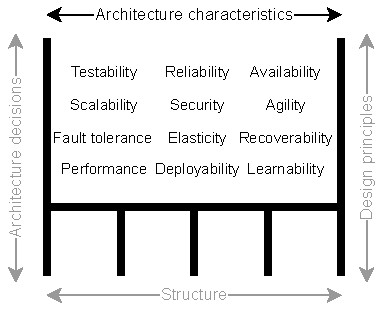
\includegraphics[width=1\textwidth]{img/ArchitectureCharacteristics}}\\ % Pfad
		\source{\cite[Eigene Darstellung in Anlehnung an][17]{Ford2020}} % Quelle
		\label{fig:ArchitectureCharacteristics}
	\end{minipage}
\end{figure}

Einige Merkmale schließen sich gegenseitig aus, wie es beispielsweise bei hoher \textit{Konsistenz}, hoher \textit{Verfügbarkeit} und hoher \textit{Ausfalltoleranz} in einem verteilten System der Fall ist. Die Unmöglichkeit diese drei \textit{Architekturmerkmale} gleichzeitig in einem verteiltem System zu garantieren, wird als \textit{CAP-Theorem} bezeichnet. Die Abkürzung CAP steht für die englischen Architekturmerkmale \textit{Consistency}, \textit{Availability} und \textit{Partition tolerance}.\footnote{\cite[vgl.][]{IBM2019}}

Der dritte Faktor sind die \textit{Architekturentscheidungen}, welche für eine Software relevant sind. Ein Softwarearchitekt gibt Regeln für das System vor, welche eingehalten werden müssen. Beispielsweise wird bei einer Schichtenarchitektur entschieden, dass nur die Business- und Serviceschichten die Datenbankschicht erreichen dürfen. Die Präsentationsschicht hingegen darf dies nicht. Diese Regeln setzen Grenzen für das System und weisen die Entwickler an, wie sie die Anwendung zu realisieren haben.\footnote{\cite[vgl.][17]{Ford2020}} Diese Regeln dürfen, im Gegensatz zu Best Practices, nicht verletzt werden.

Der letzte Aspekt der Softwarearchitektur sind \textit{Designprinzipien}. Diese beinhalten im Gegensatz zu den strikten Regeln, welche bei den Architekturentscheidungen aufgestellt wurden, eher Empfehlungen und Best Practices, welchen gefolgt werden sollte. Ein beispielhaftes Designprinzip wäre es, sofern möglich, immer auf asynchrone Kommunikation zu setzen.\footnote{\cite[vgl.][18\psq]{Ford2020}}

\textbf{Architekturstruktur MVVM}\\
Eine mögliche Architekturstruktur für Webanwendungen ist das \textit{\gls{MVVM}} Entwurfsmuster, welches eine Variante des \textit{\gls{MVC}} Entwurfsmusters darstellt und in vielen Web Frameworks verwendet wird, wie bspw. \textit{Angular}, \textit{Vue.js} oder \textit{React}.

In der nachfolgenden \cref{fig:MVVM} ist das \textit{\gls{MVVM}} Pattern dargestellt, wie es beispielsweise bei Angular eingesetzt wird.

\begin{figure}[hbt!]
	\begin{minipage}[t]{1\textwidth}	
		\caption{MVVM Pattern}
		\frame{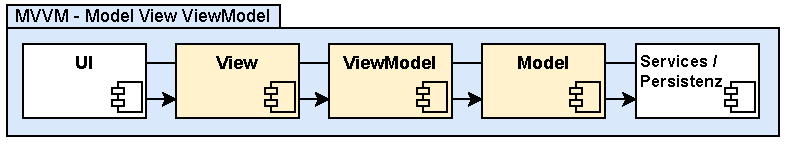
\includegraphics[width=1\textwidth]{img/mvvm}}\\ % Pfad
		\source{\cite[Eigene Darstellung in Anlehnung an][94]{Tremp2021}} % Quelle
		\label{fig:MVVM}
	\end{minipage}
\end{figure}

Das \textit{\gls{MVVM}} Muster besteht aus drei zentralen Komponenten: \textit{Datenmodell (Model)}, \textit{Präsentation (View)} und \textit{Programmsteuerung (ViewModel)}. Das \textit{ViewModel} beinhaltet die Attribute der Geschäftsobjekte, welche von der \textit{View} bei Bedarf konsumiert und angezeigt werden können. Das \textit{Model} beinhaltet die Logik und kann, durch geänderte Daten, Änderungen an der \textit{View} auslösen. Die \textit{View} repräsentiert den Inhalt, der in dem \gls{UI} angezeigt wird. Sie nimmt Nutzerinteraktionen entgegen und steht in bidirektionaler Kommunikation mit dem \textit{ViewModel}, um Werte anzuzeigen oder Input weiter zu reichen.\footnote{\cite[vgl.][95\psq]{Tremp2021}}

\textbf{Designprinzip DDD}\\
Bei dem Designprinzip des \textit{\gls{DDD}} wird eine große Anwendung in kleine, nach Fachlichkeit getrennte, Domänen aufgeteilt. Die Domänen können anhand ihres Nutzens und der Nutzer, welche mit ihr interagieren, identifiziert werden. Eine Domäne ist selbstständig und abgekapselt gegenüber anderen Domänen. Komplexe Fachlichkeiten können in Sub-Domänen einer Domäne abgebildet werden.\footnote{\cite[vgl.][4\psq]{Steyer2020}}

\subsubsection{Angular Frontend}\label{sec:AngularFrontend}

Im Jahr 2009 wurde mit \textit{AngularJS} ein Web Framework für dynamische Webanwendungen veröffentlicht.\footnote{\cite[vgl.][15]{Clow2018}} Angular Versionen sind nach \textit{\gls{SV}} benannt. \textit{AngularJS} bezeichnet das Web Framework Angular in der Major Version 1. Seit der Major Version 2 wird das Web Framework generell als Angular bezeichnet.\footnote{\cite[vgl.][]{Angular2022b}} Zum aktuellen Zeitpunkt (Q1/2022) ist Angular 13, welches im November 2021 erschienen ist, die aktuellste Version.\footnote{\cite[vgl.][]{Thompson2021}}

Durch das Web Framework Angular kann eine \textit{\gls{SPA}} realisiert werden. Bei einer \textit{\gls{SPA}} sind alle Inhalte auf einer einzigen Seite erreichbar, deren Bereiche dynamisch im Browser des Clients nachgeladen werden. Bei Angular wird die Steuerung der angezeigten Inhalte durch den Angular Router vorgenommen. Dieser kann Routen auch nur autorisierten Nutzern ermöglichen und somit Berechtigungslogik abbilden.\footnote{\cite[vgl.][]{Angular2022c}}

Angular Anwendungen sind modular aufgebaut und in Module getrennt. Ein Angular Modul gruppiert Angular Komponenten und Services, welche zu einer Domäne gehören. Angular Module können exportiert werden. Dadurch können Module andere exportierte Module importieren, um deren Funktionen einzubinden.\footnote{\cite[vgl.][]{Angular2022d}}

Eine Angular Komponente stellt eine View dar, welche aus Anzeige, Logik und Styling besteht und damit die drei Technologien verwendet, welche zu Beginn in \cref{sec:Webentwicklung} erläutert wurden.\footnote{\cite[vgl.][]{Angular2022e}} Die Darstellung und Änderung der Inhalte erfolgt über das \gls{MVVM} Pattern. Eine Angular Komponente ist Teil eines Angular Modules und kann von anderen Komponenten in dem Modul referenziert und verwendet werden.

Damit Komponenten untereinander kommunizieren und auf gemeinsam genutzte Daten oder Logik zugreifen können, gibt es Angular Services. Durch Services wird außerdem die Logik, welche zu der View der Komponente gehört, von anderen Operationen getrennt. Dadurch beinhaltet die Komponente nur noch die eigene relevante Logik. Services können durch Konstruktoren Dependency Injection in der Komponente verfügbar gemacht werden und sind anschließend referenzierbar.\footnote{\cite[vgl.][]{Angular2022f}}

Der Code von Angular Applikationen wird durch \textit{webpack} als Modulbundler zu einer \gls{JS} Datei zusammengefasst und anschließend zum Laden an den Client bereitgestellt. Webpack erstellt Pakete, welche die notwendigen \gls{HTML}, \gls{CSS} und \gls{JS} Dateien enthalten. Ebenfalls werden die Referenzen zu eventuellen Assets gesetzt, welche ebenfalls mit veröffentlicht werden. Es werden die Import-Statements jeder Datei gelesen und anhand dieser eingebundenen Dependencies ein zusammenhängendes Bundle von benötigten Bibliotheken erstellt. Die relevante Konfiguration wird in der \texttt{webpack.config.js}-Datei definiert.\footnote{\cite[vgl.][]{Angular2022g}} 

\subsection{Microservices}\label{sec:Microservices}

In diesem Abschnitt werden die Grundlagen zu Microservices erklärt. Microservices sind ein umfangreiches Thema, welches bei ganzheitlicher Betrachtung den Rahmen der Arbeit überschreiten würde. Daher werden nachfolgend nur die Grundlagen erklärt und anschließend Abgrenzungen und Gemeinsamkeiten zu Microfrontends erläutert.

Microservice-Architekturen zählen momentan zu den gefragtesten Technologien in der Softwareentwicklung \footnote{Siehe \cref{fig:StatistikMicroServices} in Anhang \ref{app:Bilder}} und sind nach der Lünendonk Studie 2021 \enquote{Cloud-native Software Development} bei zwei drittel der repräsentativen Unternehmen im Einsatz.\footnote{\cite[vgl.][]{Lünendonk2021}}

Sam Newman definiert Microservices wie folgt: \enquote{Microservices are independently releasable services that are modeled around a business domain.}\footnote{\cite[][18]{Newman2021}}

In der nachfolgenden \cref{fig:MicroservicesFeBe} ist der Unterschied zwischen einer monolithischen Anwendung und einer Microservice-Architektur mit einem monolithischen Frontend dargestellt.

\newpage
\begin{figure}[hbt!]
	\centering
	\begin{minipage}[t]{0.7\textwidth}	
		\caption{Unterschiede monolithische Anwendung zu Microservices}
		\frame{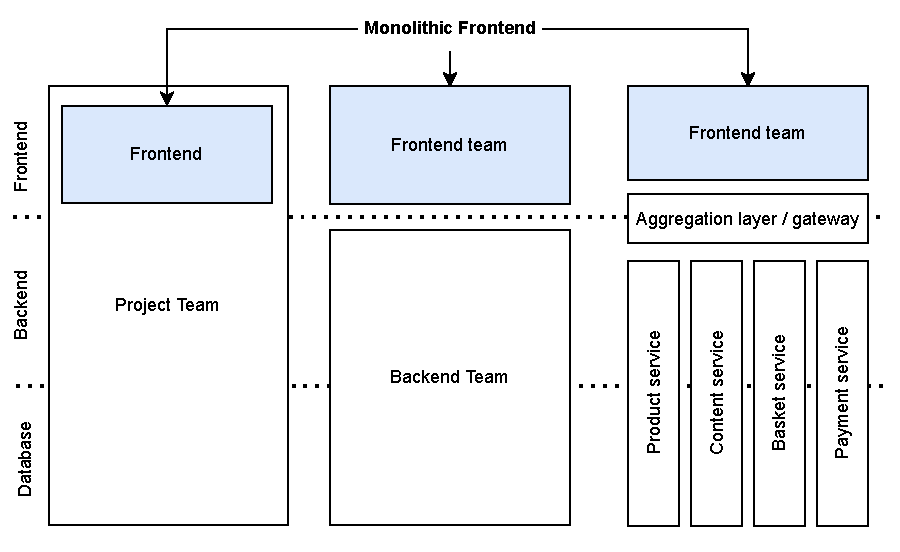
\includegraphics[width=1\textwidth]{img/MicroservicesFeBe}}\\ % Pfad
		\source{\cite[Eigene Darstellung in Anlehnung an][13]{Geers2020}} % Quelle
		\label{fig:MicroservicesFeBe}
	\end{minipage}
\end{figure}

Während die monolithische Anwendung links in der Abbildung das Frontend und das Backend ganzheitlich und ohne Trennungen beinhaltet, kann alternativ das in sich monolithische Frontend von dem monolithischen Backend getrennt sein. Bei einer Microservice-Architektur ist das Frontend ebenfalls vom Backend getrennt, welches wiederum in einzelne funktionale Blöcke aufgeteilt ist, die sogenannten Microservices. Ein Microservice ist durch ein \textit{\gls{API}} aufrufbar und beinhaltet die Logik einer Domäne.

Ein Microservice kann durch die dedizierte Verantwortung einer Domäne unabhängig veröffentlicht, sowie eigenständig getestet und individuell skaliert werden.\footnote{\cite[vgl.][]{Thoenes2015}} Dies ist bei einer monolithischen Anwendung nicht gegeben. Generell können sieben Prinzipien von Microservices herausgestellt werden, durch die sie sich von monolithischen Lösungen abgrenzen.\footnote{\cite[vgl.][16]{Mezzalira2021}} Diese werden nachfolgend erläutert.

\textbf{Modeled Around Business Domains}\\
Nach dem Prinzip des \gls{DDD} ist die Softwarelösung in fachliche Domänen aufgeteilt. Jeder Microservice repräsentiert eine eigene Domäne. Dies hat den Vorteil, dass das System klar strukturiert ist. Das verantwortliche Team der Domäne kennt die Grenzen der eigenen Verantwortung, da diese innerhalb ihrer Domäne liegt. Die Verantwortung anderer Domänen liegt bei anderen Teams.\footnote{\cite[vgl.][16\psq]{Mezzalira2021}}

\textbf{Culture of Automation}\\
Eine hoher Automatisierungsgrad ist bei einer Microservice-Architektur essentiell. Weil die Microservices unabhängig voneinander veröffentlicht werden sollen, empfiehlt es sich alle benötigten Schritte im \textit{\gls{CI/CD}} Prozess zu automatisieren.\footnote{\cite[vgl.][17]{Mezzalira2021}} So kann das Team, welches bspw. für die Werbung verantwortlich ist, seinen Microservice automatisiert neu veröffentlichen. Es muss sich nicht mit den anderen Teams absprechen, solange keine breaking Changes veröffentlicht werden. Es ist nur der eigene Microservice kurzfristig von einem Ausfall während des Veröffentlichungsprozesses betroffen, was für eine starke Unabhängigkeit spricht.

\textbf{Hide Implementation Details}\\
Um Abhängigkeiten zu vermeiden werden alle nicht benötigten Features und Schnittstellen gegenüber anderen Domänen versteckt. Es werden nur benötigte Funktionen über \gls{API}s bereitgestellt. Dadurch behält das Team des Microservices den Überblick, welche Abhängigkeiten zu anderen Domänen bestehen und kann Änderungen bewusst durchführen, ohne bestehende andere Microservices zu beeinflussen.\footnote{\cite[vgl.][17]{Mezzalira2021}}

\textbf{Decentralize Governance}\\
Bei monolithischen Anwendungen werden Architekturentscheidungen ganzheitlich für das gesamte System gefällt, obwohl diese Entscheidung eventuell nicht für jede Domäne optimal ist. Bei Microservices kann jedes Team seine eigenen Entscheidungen fällen. Ob sie beispielsweise synchron oder asynchron kommunizieren und welche Datenbanktechnologie eingesetzt wird, ist jedem Team selber überlassen. Dies sorgt dafür, dass in jeder Domäne die optimale Lösung für den jeweiligen Anwendungsfall zu finden ist. Dennoch müssen übergreifende Entscheidungen und Rahmenbedingungen vorgegeben sowie Standards eingehalten werden.\footnote{\cite[vgl.][17]{Mezzalira2021}}

\textbf{Deploy Independently}\\
Individuelles Deployment ist durch eine hohe Automatisierungsrate zeitsparend realisierbar. Wenn jeder Microservice eine eigene Deploymentpipeline hat, können einzelne Domänen bei Bedarf in einer neueren Version veröffentlicht werden, ohne das andere Domänen beeinträchtigt werden. Bei einer monolithischen Anwendung muss das gesamte System zusammen veröffentlicht werden, was zu einer Ausfallzeit führt und in Summe länger dauert. Microservices können einzeln schneller veröffentlicht werden und bei Bedarf ebenfalls schnell wieder auf einen funktionierenden Stand zurückgerollt werden.\footnote{\cite[vgl.][17]{Mezzalira2021}} 

Das unabhängige Veröffentlichen und ein hoher Automatisierungsgrad im Prozess der Veröffentlichung haben Synergieeffekte, weil der Releaseprozess dadurch pro Durchführung weniger Zeitaufwand benötigt.

\textbf{Isolate Failure}\\
Eine Folge der Auftrennung des monolithischen Backends in einzelne Microservices ist eine erhöhte Ausfallsicherheit. Bei einer monolithischen Anwendung ist das ganze System von einem Ausfall betroffen, bei einer Microservice-Architektur lediglich die Features der betroffenen Domäne. Kunden können weiterhin die Features der anderen Domänen nutzen und bemerken den Ausfall der betroffenen Domäne im besten Fall gar nicht.\footnote{\cite[vgl.][18]{Mezzalira2021}}

\textbf{Highly Observable}\\
Eine der Herausforderungen einer verteilten Microservice-Architektur ist es, den Überblick über alle Domänen zu behalten. Eine monolithische Anwendung als Gesamtsystem ist einfacher zu Überblicken und kann schneller um neue domänenübergreifende Anfragen erweitert werden. Bei einer Microservice-Architektur ist dies mit mehr Aufwand verbunden, welcher aber durch die gewonnene Flexibilität zu rechtfertigen ist.\footnote{\cite[vgl.][18]{Mezzalira2021}} Der höhere Aufwand entsteht durch die Abkapselung der anderen Domänen. Es ist für ein Team einer Domäne nicht direkt ersichtlich, von welchen Features anderer Domänen profitiert werden kann.

Zusammenfassend bringt eine Microservice-Architektur einige Vorteile gegenüber einer monolithischen Architektur. Allerdings ist eine Umstrukturierung der internen Organisation erforderlich, damit Teams unabhängig voneinander sind und Domänentrennung bei Erhaltung des Gesamtüberblickes realisiert werden können.\footnote{\cite[vgl.][18]{Mezzalira2021}}

Die Prinzipien von Microservices lassen sich auf Microfrontends übertragen, was im nachfolgenden \cref{sec:MicrofrontendArchitektur} getan wird.

\subsection{Microfrontend-Architektur}\label{sec:MicrofrontendArchitektur}

In diesem Kapitel werden die Grundlagen von Microfrontends erläutert. Dazu werden zunächst die Gemeinsamkeiten von Microfrontends gegenüber Microservices erläutert sowie Unterschiede abgegrenzt. Anschließend wird das Konzept einer Microfrontend-Architektur präsentiert und Microfrontends aus technischer sowie organisatorischer Sicht vorgestellt.

Microfrontends sind ein möglicher Ansatz der Softwarearchitektur einer Webseite. Anstatt eines monolithischen Frontends ist das Frontend in kleinere, fokussierte Subsysteme aufgeteilt, welche von einem eigenen Team betrieben werden, das sich auch um das dazugehörige Backend kümmert.\footnote{\cite[vgl.][21\psq]{Geers2020}}

In der nachfolgenden \cref{fig:fragments} sind drei Microfrontends dargestellt. Diese werden jeweils von drei verschiedenen Teams betreut und können in unterschiedlichen Web-Frameworks entstanden sein.

\begin{figure}[hbt!]
	\centering
	\begin{minipage}[t]{0.8\textwidth}	
		\caption{Verschiedene voneinander unabhängige Microfrontends}
		\frame{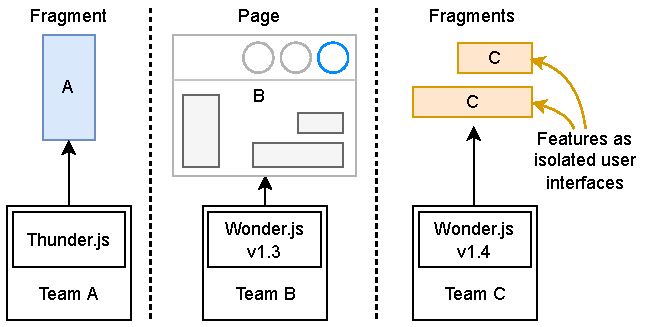
\includegraphics[width=1\textwidth]{img/IsolatedFragments}}\\ % Pfad
		\source{\cite[Eigene Darstellung in Anlehnung an][8]{Geers2020}} % Quelle
		\label{fig:fragments}
	\end{minipage}
\end{figure}

Team A und C steuern jeweils Fragmente bei. Team B ist verantwortlich für die eigentliche Seite, welche die anderen Fragmente später einbindet, und lässt Platzhalter an den Stellen frei, wo die Fragmente in Zukunft platziert werden sollen. Das Zusammenfügen der einzelnen Fragmente auf der Seite erfolgt durch die Konfiguration von Team B und ist nachfolgend in der \cref{fig:frontendintegration} dargestellt.

\newpage 
\begin{figure}[hbt!]
	\centering
	\begin{minipage}[t]{0.8\textwidth}	
		\caption{Frontend Integration der einzelnen Microfrontends}
		\frame{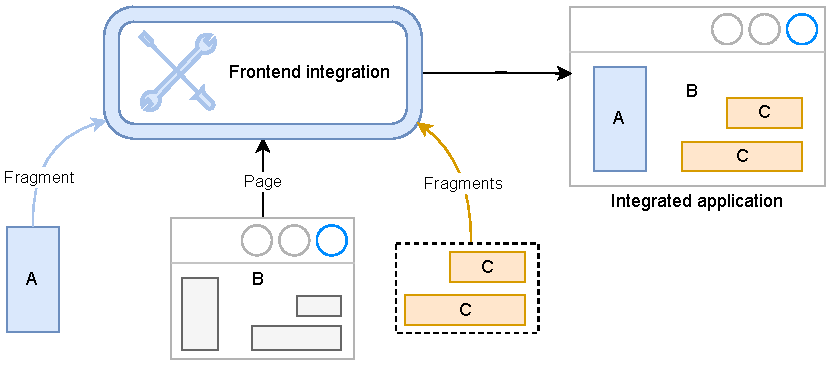
\includegraphics[width=1\textwidth]{img/FrontendIntegration}}\\ % Pfad
		\source{\cite[Eigene Darstellung in Anlehnung an][10]{Geers2020}} % Quelle
		\label{fig:frontendintegration}
	\end{minipage}
\end{figure}

Die Fragmente und die Seite mit den noch leeren Platzhaltern werden durch die sogenannte \textit{Frontend integration} zusammengesetzt und es entsteht eine Web-Anwendung bestehend aus mehreren Microfrontends, was für den Anwender idealerweise nicht ersichtlich ist. Ein Beispiel für eine zusammengesetzte Microfrontend-Applikation ist in der nachfolgenden \cref{fig:TractorStoreMicrofrontend} dargestellt.

\begin{figure}[hbt!]
	\centering
	\begin{minipage}[t]{0.8\textwidth}	
		\caption{Eine aus Microfrontends bestehende Webseite}
		\frame{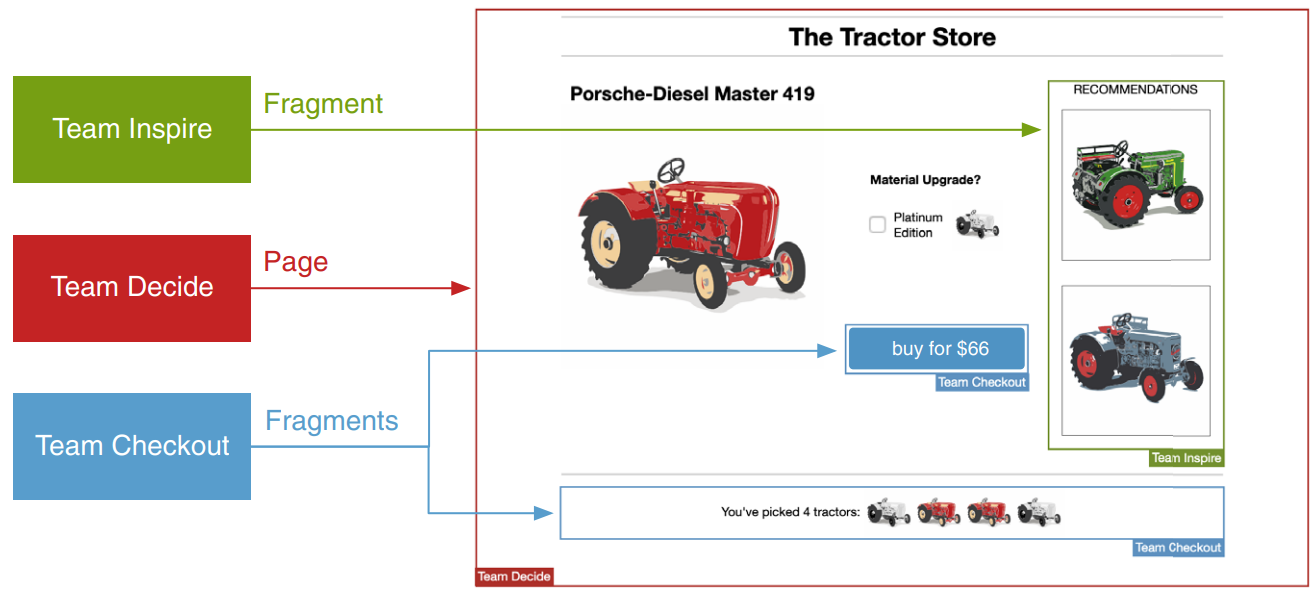
\includegraphics[width=1\textwidth]{img/TractorStoreMicrofrontend}}\\ % Pfad
		\source{\cite[][9]{Geers2020}} % Quelle
		\label{fig:TractorStoreMicrofrontend}
	\end{minipage}
\end{figure}

Das Frontend des beispielhaften Traktorshops ist aus den Fragmenten drei verschiedener Teams zusammengesetzt. \textit{Team Decide} stellt die eigentliche Seite mit den Platzhaltern zur Verfügung, in welche die Fragmente der Teams \textit{Inspire} und \textit{Checkout} eingebunden werden. Für den Shopbenutzer ist diese Trennung in drei Teams nicht ersichtlich und die Webseite erscheint als eine zusammengehörige Komponente.

\subsubsection{Gemeinsamkeiten und Abgrenzungen zu Microservices}\label{sec:AbgrenzungenMicroservices}

Im \cref{sec:Microservices} wurden das Konzept, die Vorteile und Anwendungsfälle von Microservices vorgestellt. In diesem Abschnitt werden weiterführend Abgrenzungen und Gemeinsamkeiten von Microservices gegenüber Microfrontends herausgearbeitet, bevor im nachfolgenden \cref{sec:MicrofrontendArchitekturTechnisch} die Microfrontend-Architektur erklärt wird.

Microfrontends und Microservices unterscheiden sich durch ihren Scope. Microservices sind für das Backend einer Anwendung zuständig und befinden sich hinter der \gls{API}. Microfrontends sind für das Frontend einer Anwendung zuständig und rufen die \gls{API} auf.

Abseits vom Scope gibt es aber viele Gemeinsamkeiten. So lassen sich die Prinzipien von Microservices, welche im vorherigen Abschnitt dargestellt wurden, auf Microfrontends übertragen.\footnote{\cite[vgl.][18-20]{Mezzalira2021}} In Anhang \ref{app:Bilder} in \cref{fig:MonolithicMicrofrontend} ist eine Gegenüberstellung von einem monolithischen Frontend zu einer Applikation mit Microfrontends zu sehen. Bei der Applikation mit Microfrontends ist das Frontend in mehrere unabhängige und nach Fachlichkeit getrennte Teile aufgetrennt, genau wie es bei Microservices im Backend der Fall ist. Dadurch sind vertikale Teams in der Lage die gesamte Verantwortung in ihrer Domäne zu übernehmen. Beispielsweise ist das \textit{Product Team} für den \textit{Product Microservice} sowie für das \textit{Product Microfrontend} zuständig und verwaltet somit die gesamte Produkt-Domäne.

\subsubsection{Microfrontend-Architektur aus technischer Sicht}\label{sec:MicrofrontendArchitekturTechnisch}

\enquote{Microfrontends are not appropriate for every application because of their nature and the potential complexity they add at the technical and organizational levels.}\footnote{\cite[][20]{Mezzalira2021}}

Damit die Vorteile von Microfrontends genutzt werden können, sollten die Anforderungen geprüft und die Architektur dahingehend geplant werden. Eine Microfrontend-Architektur kann nach Mezzalira durch vier Prinzipien beschrieben werden. 

Die vier Prinzipien lauten: \textit{business domain representation}, \textit{autonomous codebase}, \textit{independent deployment} und \textit{single-team ownership}. Ein Microfrontend repräsentiert dementsprechend eine Geschäftsdomäne, welche autonom entwickelt sowie unabhängig veröffentlicht werden kann und von einem eigenen Team betreut wird.\footnote{\cite[vgl.][23]{Mezzalira2021}}

Nachfolgend wird das sogenannte \textit{Microfrontend Decision Framework} vorgestellt. Es beschreibt Kriterien, anhand welcher passende Architekturentscheidungen für die Anwendung getroffen werden können und beinhaltet vier Kernaspekte:\footnote{\cite[vgl.][24]{Mezzalira2021}}

\begin{compactitem}
	\item Einheitliche Definitionen in der eigenen Architektur
	\item Zusammensetzung
	\item Weiterleitung
	\item Kommunikation untereinander
\end{compactitem}

Die einzelnen Aspekte werden nachfolgend im Detail erklärt, weil sie wichtige Grundlagen zum Verständnis von Microfrontend-Architekturen bilden.

\textbf{Einheitliche Definition von Microfrontends in der eigenen Architektur}\\
Zunächst muss ein einheitliches Verständnis von einem Microfrontend gewonnen werden. Dafür wird unterschieden, ob es sich um eine vertikale Trennung in Domänen nach dem \gls{DDD} Konzept, oder um eine horizontale Trennung von mehreren Microfrontends auf der gleichen Seite, wie in der nachfolgenden \cref{fig:HorizontalVerticalSplit} dargestellt, handelt.

\begin{figure}[hbt!]
	\begin{minipage}[t]{1\textwidth}	
		\caption{Horizontale und vertikale Trennung von Microfrontends}
		\frame{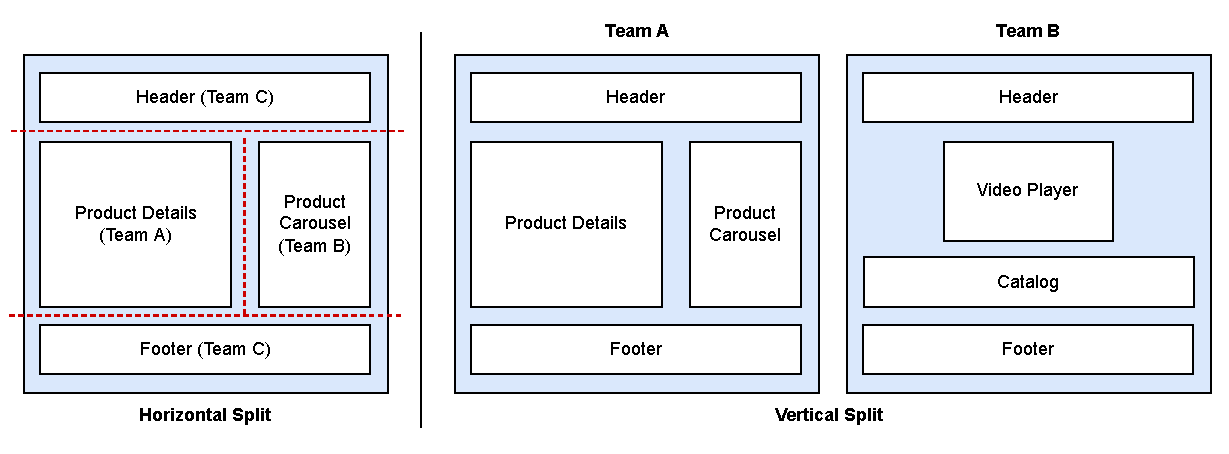
\includegraphics[width=1\textwidth]{img/HorizontalVerticalSplit}}\\ % Pfad
		\source{\cite[Eigene Darstellung in Anlehnung an][24]{Mezzalira2021}} % Quelle
		\label{fig:HorizontalVerticalSplit}
	\end{minipage}
\end{figure}

Bei dem \gls{DDD} geht es darum, die Anwendung in Fachdomänen aufzutrennen. Eine Domäne kann wiederum in mehrere Subdomänen aufgeteilt werden, welche sich in drei Typen unterscheiden lassen:\\
In \textit{funktionale Subdomänen}, welche den Hauptnutzen der Domäne repräsentieren. \\
In \textit{unterstützende Subdomänen}, welche zwar die funktionale Subdomäne unterstützen, aber keinen direkten Wert beisteuern.\\
In \textit{generische Subdomänen}, welche der übergreifenden Plattform dienen und den Prozess abrunden. Sie haben keinen direkten Bezug zur Domäne, sind aber für die Erfüllung des übergreifenden Nutzens relevant (bspw. die Authentifizierung auf einer Webseite).\footnote{\cite[vgl.][24\psqq]{Mezzalira2021}} 

Im Falle der in \cref{fig:HorizontalVerticalSplit} dargestellten vertikalen Trennung wird in die Domänen \textit{Video} und \textit{Produkt} unterschieden, welche jeweils von einem Team betreut werden. Die Teams mit ihren Domänen sind voneinander unabhängig und abgekapselt. Sollten Zugriffe domänenübergreifend notwendig sein, werden diese über ein \gls{API} realisiert.

\textbf{Zusammensetzung von Microfrontends}\\
Ebenfalls muss vorab entschieden werden, wann die Microfrontends zusammengesetzt werden (engl. \textit{composition}). Dies kann an drei verschiedenen Stellen geschehen:\footnote{\cite[][29]{Mezzalira2021}}
\begin{compactitem}
	\item \textit{Client-side Composition}
	\item \textit{Edge-side Composition}
	\item \textit{Server-side Composition}
\end{compactitem}

Bei der \textit{Client-side Composition} werden die einzelnen Microfrontends vom Client einzeln aus einem \gls{CDN}, oder falls dort nicht vorhanden, direkt aus der Quelle geladen und am Client im Browser zusammengesetzt.

Bei der \textit{Edge-side Composition} wird das Zusammensetzen der einzelnen Microfrontends im \gls{CDN} vollzogen und die Anwendung als Ganzes an den Client ausgeliefert.

Die \textit{Server-side Composition} hingegen setzt die Microfrontends bereits auf einem Server zusammen und gibt sie als Ganzes an das \gls{CDN} weiter, welches die Seite zwischenspeichert und anschließend an den Client ausliefert.

\textit{Client-side} und \textit{Server-side Composition} werden in den \crefrange{sec:ServerSideComposition}{sec:ClientSideComposition} ausführlicher behandelt. Auf eine detailliertere Erklärung von \textit{Edge-side Composition} wird verzichtet, da es dem Konzept der\textit{ Server-side Composition} ähnelt und für den weiteren Verlauf der \dokumententyp{} keine Relevanz hat.

\textbf{Weiterleitung von Microfrontends}\\
Nachdem der Ort der Zusammenstellung der Microfrontends bestimmt wurde, muss eine Technik gewählt werden, um zwischen den Ansichten verschiedener Microfrontends zu wechseln. Bezogen auf den vorherigen Punkt \textit{Zusammensetzung} muss entschieden werden, ob das Weiterleiten (engl. \textit{Routing}) auf dem Server, dem \gls{CDN} oder am Client passiert.

Wenn die Anwendung auf dem Server zusammengesetzt wird, muss sie auch dort gerouted werden, weil sich die Logik sowie die anderen Ansichten serverseitig befinden. Die gerouteten Ansichten können dann vom \gls{CDN} zwischengespeichert werden, wenn sich die Ansichten nicht individuell pro Mandant oder User unterscheiden.\footnote{\cite[vgl.][31]{Mezzalira2021}}

Bei dem Einsatz von \textit{Edge-side Composition} wird das Routing über \gls{URL} realisiert und die Microfrontends werden vom \gls{CDN} Server zusammengesetzt.\footnote{\cite[vgl.][32]{Mezzalira2021}} Es besteht in diesem Fall nicht viel Entscheidungsfreiraum beim Routing, was einer der Gründe ist, warum \textit{Edge-side Composition} im Rahmen der Thesis nicht weiter verfolgt wird.

Das Routing am Client durchzuführen bringt die meiste Flexibilität, da die einzelnen Microfrontends nach Bedarf und individueller Konfiguration des Clients geladen und zwischengespeichert werden können.

Die Art des clientseitigen Routings ist in \gls{SPA}s wiederzufinden, welche bereits vorher in \cref{sec:AngularFrontend} beschrieben wurden. Eine \gls{SPA} kann als \textit{Application Shell} fungieren, indem sie abhängig des aktuellen Router- und Nutzerstatus andere Microfrontends einbindet und anzeigt. Die \textit{Application Shell}s bieten Querschnittsaspekte, wie bspw. Routing, Authentifizierung und Autorisierung, von welchen die Microfrontends profitieren können und über die ein komplexes, individuelles Routing abgebildet werden kann. Die Konzepte der \textit{Application Shell} und der eingebundenen Microfrontends werden im nachfolgenden \cref{sec:Portalapplikationen} ausführlich behandelt.

Das clientseitige Routing kann auch ohne eine \gls{SPA} lediglich über \gls{URL}s realisiert werden, zwischen welchen der Benutzer navigieren kann.\footnote{\cite[vgl.][32]{Mezzalira2021}} Dabei springt der Benutzer aber von Seite zu Seite, verliert eventuell gespeicherte Informationen und wird mit Ladezeiten je Seite konfrontiert.

\textbf{Kommunikation von Microfrontends untereinander}\\
Optimalerweise laufen Microfrontends vollkommen autark und haben nach dem \gls{DDD} Prinzip keine Überschneidungen zu anderen Domänen. Dies ist bei größeren Applikationen aber nicht gegeben, weil beispielsweise Microfrontends auf die Nutzerdomäne zugreifen müssen, um Informationen über den aktuellen Benutzer erhalten zu können.

Besonders bei mehreren Microfrontends auf der gleichen Seite ist das Verwalten einer konsistenten und kohärenten \gls{UX} herausfordernd. Zusätzlich erschwert die Domänenverwaltung durch verschiedene Teams das Kommunizieren von Microfrontends untereinander.\footnote{\cite[vgl.][33]{Mezzalira2021}}

Die Kommunikation kann, bei horizontaler Trennung, über vier verschiedene Arten erfolgen: \textit{Event emitter}, \textit{Custom events}, \textit{Web Storage} oder \textit{Query Strings}. Bei vertikaler Trennung sind ist die Kommunikation nur über einen \textit{Web Storage} und \textit{Query Strings} möglich.

Sind die Microfrontends auf der gleichen Seite eingebunden, kann über Events kommuniziert werden. Eine zentrale Stelle (bspw. die \textit{Application Shell}) versendet Events und Microfrontends können auf diese Eventbenachrichtigungen reagieren. Dies ist über das \textit{CustomEvent} Interface von Javascript möglich.\footnote{\cite[vgl.][]{MDNWebDocs2022b}}

Die Daten können ebenfalls über \textit{Event Emitter} geteilt werden, wie in \cref{fig:MFSharingDataEventEmitter} in Anhang \ref{app:Bilder} dargestellt. Dafür muss ein \gls{Eventbus} in jedes Microfrontend eingefügt werden, auf welchem Nachrichten versendet werden können.\footnote{\cite[vgl.][33]{Mezzalira2021}}

Eine weitere Möglichkeit zum Datenaustausch ist das Teilen von Informationen über einen gemeinsamen \textit{Web Storage} (siehe \cref{fig:MFSharingDataWebStorage} in Anhang \ref{app:Bilder}). Es wird ein \textit{Web Storage} verwendet, welcher von Microfrontends der gleichen Subdomain erreicht werden kann. Dort liegen Informationen des Benutzers, auf welche das Microfrontend zurückgreifen kann.\footnote{\cite[vgl.][34]{Mezzalira2021}}

\textbf{Zusammenfassung Microfrontend Decision Frameworkes}\\
In der nachfolgenden \cref{tab:ZusammenfassunfMFFramework} ist eine Zusammenfassung des Microfrontend Decision Frameworkes dargestellt.

\begin{table}[hbt]
	\centering
	\begin{minipage}[t]{1\textwidth} % Breite, z.B. 1\textwidth		
		\caption{Zusammenfassung des Microfrontend Decision Framework} % Überschrift
		\begin{tabular}{|
				l|ccc|}
			\midrule
			\textbf{Microfrontend definition\quad\quad\quad}&\textbf{Composition}&\textbf{Routing}&\textbf{Communication}\\
			\midrule
			\multirow{4}{*}{Horizontal}
			&Client side 	&Client side	&Event emitter\\ 
			&Server side 	&Server side	&Custom events\\
			&Edge side 		&Edge side		&Web storage\\
			&				&				&Query strings\\						
			\midrule
			\multirow{3}{*}{Vertical}
			&Client side	&Client side	&Web Storage\\ 
			&Server side	&Server side	&Query Strings\\
			& 				&Edge side		&\\
			\midrule
		\end{tabular}
		\newline
		\source{\cite[Eigene Darstellung in Anlehnung an][35]{Mezzalira2021}}
		\label{tab:ZusammenfassunfMFFramework}
	\end{minipage}
\end{table}

Die Tabelle zeigt, dass nicht alle Ausprägungen einer Kategorie miteinander kombinierbar sind. Die erste Entscheidung muss bezüglich der Definition getroffen werden. Eine vertikale Definition hat zur Folge, dass beim Routing und bei der Kommunikation weniger Optionen verfügbar sind.

Die Vorteile und Nachteile lassen sich aus den eingangs erklärten Prinzipien von Microfrontends ableiten und werden zur Übersicht nachfolgend noch einmal erklärt.

\textbf{Vorteile gegenüber einem monolithischen Frontend}\\
Der primäre Vorteil einer Microfrontend-Architektur ist die gewonnene Flexibilität. Jedes Team ist selbstverantwortlich für ihr zugewiesenes Microfrontend. Sie sind in der Lage selbstständig Architekturentscheidungen zu treffen, welche zu ihren Aufgaben und Problemen passen. Ebenfalls können bei Bedarf neue Softwarestände durch die eigenen Pipelines veröffentlicht werden, ohne andere Microfrontends zu beeinflussen. 

Des Weiteren wird das Microfrontend nicht durch andere Ausfälle beeinflusst. Hat beispielsweise das für die Werbung einer Seite verantwortliche Team eine Störung, kann das Team verantwortlich für die Kaufabwicklung ohne Auswirkungen weiter agieren.\footnote{\cite[vgl.][19\psq]{Mezzalira2021}} So ist das nicht direkt betroffene Team weiterhin nicht abhängig und der Benutzer bemerkt die Störung außerhalb der betroffenen Domäne ebenfalls nicht.

Darüber hinaus ist durch die Trennung nach Domänen in eigenverantwortliche Teams eine klare Strukturierung der Verantwortung gegeben, welche bei der Organisation der Gesamtwebseite von Vorteil ist. Auch ist eine verbesserte Skalierbarkeit gegeben, sodass modulare Microfrontends mehrfach nach Bedarf eingebunden werden können (\textit{\gls{DRY}} Prinzip).

\textbf{Nachteile gegenüber einem monolithischen Frontend}\\
Nachteile einer Microfrontend-Architektur gegenüber einem monolithischen Ansatz sind in den Aspekten Redundanz, Konsistenz und Heterogenität zu finden.\footnote{\cite[vgl.][17]{Geers2020}}

\textbf{Redundanz}\\
In Microfrontend-Architekturen sind Redundanzen nicht zu vermeiden. So hat jedes Team ein eigenes Repository, eine eigene Deployment-Pipeline und einen eigenen Ort zum Hosten des Microfrontends.\footnote{\cite[vgl.][17\psq]{Geers2020}} Ein eigenes Repository ist zwar hilfreich, um sich als Team selbstständiger zu organisieren, aber es besteht auch die Möglichkeit ein Monorepo übergreifend zu verwenden. Dort sind alle Microfrontends der Applikation gleichzeitig enthalten. Alle Microfrontends können auf geteilte Bibliotheken in dem Monorepo zugreifen. Dies erfordert eine gute Zusammenarbeit der einzelnen Teams und eine strikte Organisation des Repositories, was mit Mehraufwand einhergeht.\footnote{\cite[vgl.][153\psq]{Mezzalira2021}}

Durch den Aspekt, dass das vorher monolithische Frontend in kleinere Fragmente aufgeteilt wurde, welche alle selbstständig lauffähig sind, kommt es zu mehrfach geladenem Code.\footnote{\cite[vgl.][19]{Geers2020}} Beispielsweise muss das Web Frontend Framework Angular für jedes Microfrontend geladen werden oder es müssen mehrere verschiedene Web Frontend Frameworks geladen werden. Bei einer monolithischen Anwendung dahingegen wird nur ein Web Frontend Framework benötigt.

\textbf{Konsistenz}\\
Der Microfrontend Ansatz verlangt, wie in \cref{fig:MicroFrontendBigPicture} zu sehen, die Aufteilung in eigenständige, vertikal agierende Teams. Diese Teams sollen nach Möglichkeit alles selbstständig betreiben, vom Frontend über das Backend bis hin zur Datenbank. Nun kann es vorkommen, dass ein Team Daten von einem anderen Team benötigt. Ein direkter Zugriff oder eine geteilte Datenbank würde die Domänentrennung verletzen. 

Aus diesem Grund muss das Team, welches Daten eines anderen Teams benötigt, die Daten replizieren. Das Replizieren von Datenbeständen ist notwendig, damit aus Gründen der Unabhängigkeit und Ausfallsicherheit auf direkte Zugriffe verzichtet werden kann.
Die Replizierung der Daten hat den Nachteil, dass Abhängig von den Replizierungsintervallen unter Umständen veraltete Datenbestände verwendet werden. Darüber hinaus werden doppelte Ressourcen (Speicher- und Rechenkapazität) benötigt.\footnote{\cite[vgl.][18]{Geers2020}} 

Auf eine Replizierung kann verzichtet werden, wenn die Schnittstellen von Domänen in begründeten Fällen doch zur Verfügung gestellt werden. Dies könnte beispielsweise bei weniger relevanten Daten der Fall sein, bei denen ein temporärer Ausfall die Kernfunktion nicht beeinträchtigt.

\textbf{Heterogenität}\\
Da die Teams unabhängig voneinander sind, steht es ihnen frei, welche Technologie sie verwenden. So können alle Microfrontends einer Applikation einheitlich in Angular 12 geschrieben sein. Es besteht aber auch die Möglichkeit verschiedene Versionen der gleichen Technologie zu verwenden. Ein Angular 11 Microfrontend kann in eine Angular 12 Application Shell eingebunden werden. 
Es können aber auch andere Web Frontend Frameworks verwendet werden, also an Stelle von Angular beispielsweise Vue.js oder React. Allerdings erschweren heterogene Technologien den Informationsaustausch der Teams untereinander und einzelne Entwickler können nicht so einfach ohne Weiterbildung zwischen den Teams wechseln. 

Einheitliches Design ist ein wichtiger Aspekt einer funktionierenden Software. Es gibt dem User das Gefühl sich durchgehend auf einer Webseite aufzuhalten. Durch ein \textit{Design System}, eine verbindliche Vorgabe zur Einhaltung eines stringenten Designs für alle beteiligten Teams der Applikation, kann eine einheitliche Webseite erschaffen werden. Auch wenn diese im Hintergrund aus vielen autonomen Microfrontends besteht. Durch die einheitlichen Vorgaben und das stringente Design wird dem Benutzer ein stimmiges \gls{UI}/\gls{UX} Erlebnis ermöglicht.\footnote{\cite[vgl.][214\psqq]{Geers2020}}

Ein \textit{Design System} kann durch einen \textit{Style Guide} realisiert werden, welcher Styles in Form von Schriftarten, Farben und Grafiken vorgibt. Alternativ kann eine \textit{Komponentenbibliothek} zur Verfügung gestellt werden, welche Elemente zum Einbinden in Microfrontends in Form von Formularelementen, Navigationselementen oder Anzeigeelementen liefert.\footnote{\cite[vgl.][215]{Geers2020}} Ein \textit{Design System} zu implementieren und zu Pflegen bedeutet jedoch Mehraufwand, welcher in Kauf genommen werden muss.

Zusammenfassend kann also gesagt werden, dass bei einer Microfrontend-Architektur die Vorteile Flexibilität, Unabhängigkeit und Übersicht nur durch Mehraufwand in der Organisation sowie Redundanz realisierbar sind. Die Nachteile sind durch Mehraufwand kompensierbar, was bei vorheriger Planung und Überprüfung der Architektur gut zu bewältigen ist.

\textbf{Wirkungsbereiche von Microfrontend-Architekturen}\\    
Microfrontend-Architekturen besitzen Vor- und Nachteile. Diese besondere Form der Softwarearchitektur ist nicht für alle Arten von Softwarelösungen geeignet. Wo diese Architekturen empfehlenswert sind und wo sie nicht gerechtfertigt sind, wird nachfolgend erläutert.

Eine Microfrontend-Architektur bietet sich für große, verteilte Softwarelösungen an. Der Bedarf nach Flexibilität und Skalierbarkeit tritt erst ab einem gewissen Umfang der Softwarelösung auf. Bei kleineren Projekten sind Kosten und Schnelligkeit entscheidender.\footnote{\cite[vgl.][19]{Geers2020}}

Die angezeigten Frontends dynamisch auszutauschen funktioniert am besten clientseitig durch \gls{SPA}s. Serverseitiges Rendering erfordert ein erneutes Laden des Inhaltes, was zwar technisch keine Herausforderung darstellt, jedoch nicht so flüssig und unbemerkt wie clientseitige Komposition abläuft. Smartphone Apps als Microfrontend zu realisieren ist schwieriger, da die Betreiber von App Stores strikte Kontrollen des Inhaltes durchführen, bei denen jedes Microfrontend in jeder Version überprüft werden müsste. Dadurch schwinden die flexiblen, unabhängigen Vorteile von Microfrontends.\footnote{\cite[vgl.][19\psq]{Geers2020}}

Eine monolithische Anwendung in viele einzelne Teile aufzutrennen bringt Vorteile und Nachteile mit sich, welche im vorherigen Abschnitt erläutert wurden. Es muss vermehrter organisatorischer Aufwand in Kauf genommen werden. Dieser entsteht durch zusätzliche Abstimmung der Teams untereinander, bspw. für einheitliche Namespaces und Trennung der Verantwortung. Die Aufteilung einer monolithischen Anwendung in ein verteiltes System sorgt für zusätzliche Komplexität. Den verantwortlichen Teams muss die gewonnene Flexibilität wichtiger sein, als der Aufwand und die Komplexität.\footnote{\cite[vgl.][20]{Geers2020}}

\enquote{Microfrontends are a sensible option when we are working on software that requires an iterative approach and long-term maintenance, when we have projects that require multiple teams to work on the same application, or when we want to replace a legacy project in an iterative way.}\footnote{\cite[][21]{Mezzalira2021}}

Eine Microfrontend-Architektur ist nicht effektiv, wenn nur wenige Entwickler an der Softwarelösung arbeiten. Außerdem müssen die Domänen und Verantwortlichkeiten der Teams gut gegeneinander abgetrennt sein, weil es ansonsten zu Unsicherheiten und Verständnisproblemen der Teams untereinander kommen kann.\footnote{\cite[vgl.][21]{Geers2020}}

\subsubsection{Microfrontend-Architektur aus organisatorischer Sicht}\label{sec:MicrofrontendArchitekturOrganisatorisch}

Eine Microfrontend-Architektur hat neben den technischen Aspekten auch organisatorische Unterschiede zu herkömmlichen Architekturen. Einige dieser Aspekte, wie vertikale Teams, notwendige Abstimmungen und geteiltes Wissen wurden bereits in den vorherigen Abschnitten beiläufig erwähnt und werden nachfolgend noch einmal strukturiert erklärt.

\textbf{Organisation der Teams}\\
Es existieren verschiedene Möglichkeiten die Teams bei einer Microfrontend-Architektur zu organisieren. In der nachfolgenden \cref{fig:TeamDepth} wird zwischen ausschließlich im Frontend agierenden Teams, Full-Stack Teams und vollständig autonomen Teams unterschieden.

\begin{figure}[hbt!]
	\centering
	\begin{minipage}[t]{0.85\textwidth}	
		\caption{Organisationsmöglichkeiten der Microfrontend Teams}
		\frame{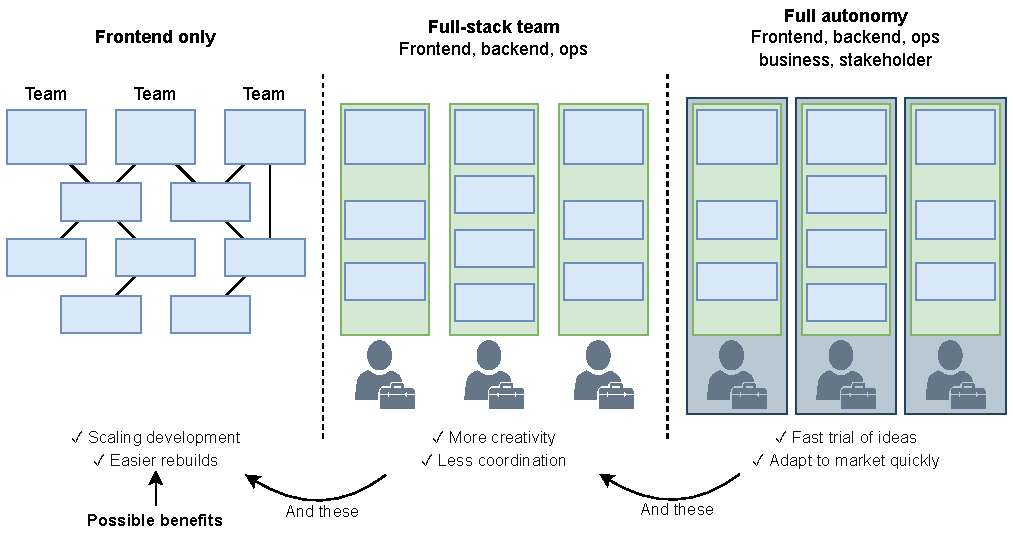
\includegraphics[width=1\textwidth]{img/TeamDepth}}\\
		\source{\cite[Eigene Darstellung in Anlehnung an][240]{Geers2020}} % Quelle
		\label{fig:TeamDepth}
	\end{minipage}
\end{figure}

Beim monolithischen Ansatz ist ein großes Team für die ganze Anwendung verantwortlich. Bei \textit{Frontend only} Teams sind es mehrere, kleine Teams, die jeweils einen bestimmten Bereich des Frontends betreuen. Dies hat den Vorteil, dass die Entwickler in den kleinen Teams sich besser mit den Fachlichkeiten auskennen.\footnote{\cite[vgl.][241]{Geers2020}}

Ebenfalls besteht die Möglichkeit die Teams vertikal aufzuteilen, wodurch jedes Team die Full-Stack Verantwortung für seinen Teilbereich hat. Dies hat den Vorteil, dass weniger Abstimmung notwendig ist, da Frontend und Backend der gleichen Domäne mitsamt der dazwischen liegenden Schnittstellen bei den selben Entwicklern liegen. Ebenfalls werden Full-Stack Teams aus Personen mit diversen fachlichen Wissensständen zusammengesetzt, was die Kreativität der Problemlösung und Qualität des Ergebnisses fördern kann.\footnote{\cite[vgl.][241]{Geers2020}}

Werden die Stakeholder auch noch in das Full-Stack-Team integriert, so kann von einem vollständig autonomen Team gesprochen werden. Wenn die Stakeholder, wie bspw. Marketing, Kunden oder Support, direkt in den Problemlösungsprozess integriert werden, kann von noch kreativeren Blickwinkeln profitiert und die \gls{TTM} noch weiter reduziert werden.\footnote{\cite[vgl.][242]{Geers2020}}

\textbf{Wissensverteilung}\\
Das Wissen übergreifend über autonome Teams hinweg zu verteilen geschieht nicht automatisch, ist aber dennoch ein wichtiger Prozess. Die Mitglieder von vertikalen Teams treffen sich in sogenannten \gls{COP}, welche horizontal organisierten Expertenkreisen entsprechen. So können Best Practices und Erfahrungen der Teams in den notwendigen technischen Tiefen der jeweiligen Spezialisierungen ausgetauscht werden. In Anhang \ref{app:Bilder} in \cref{fig:VertikaleTeamsWissensaustausch} sind drei autonome Teams dargestellt, welche sich regelmäßig in Expertenkreisen treffen und austauschen. So gibt es beispielsweise einen Expertenkreis für das Themengebiet Frontend, einen für die Datenanalyse und einen für Kubernetes als Infrastrukturplattform.

Das Konzept der \gls{COP}s besteht schon länger, als die Microfrontend-Architektur. Doch es ist bei dieser Art der Teamorganisation besonders wichtig, da der sonst bestehende natürliche Austausch innerhalb eines horizontalen Teams verloren geht. In den \gls{COP}s sollte sich auch auf Standards und Konventionen für Schnittstellen und Namespaces innerhalb eines Projektes geeignet werden.

\textbf{Verwaltung des Codes}\\
Bei klassisch monolithischen Anwendungen gibt es ein Repository für die ganze Applikation. Bei Microservices und -frontends kann es für jede Einheit ein eigenes Repository geben. Dies wird als \textit{Polyrepo} bezeichnet. Alternativ kann aber auch für das ganze Projekt nur ein Repository genutzt werden, welches dann einem \textit{Monorepo} entspricht.

Vorteile eines \textit{Monorepos} sind, dass dadurch die Absprache der Teams untereinander vereinfacht wird, weil der Code des anderen Teams direkt zugänglich ist und eingebunden werden kann. Ebenfalls kann der Code einfacher einheitlich überarbeitet werden, da alle Dateien nebeneinander verfügbar sind.\footnote{\cite[vgl.][152\psqq]{Mezzalira2021}}

\textit{Polyrepos} haben den Vorteil, dass die Autonomie gestärkt wird. Jedes Microfrontend hat sein eigenes Repository und eigene \gls{CI/CD} Pipelines angebunden. Ebenfalls können individuelle Branchingstrategien pro Team verwendet und versehentliche Abhängigkeiten vermieden werden, da Zugriffe zwischen Teams nur über definierte \gls{API}s möglich sind.\footnote{\cite[vgl.][156\psqq]{Mezzalira2021}}

Das Konzept des \textit{Monorepos} wird im Microfrontend-Umfeld kontrovers diskutiert. Einige Autoren sehen Vorteile durch Wiederverwendbarkeit und vereinfachte Abhängigkeiten.\footnote{\cite[vgl.][152\psqq]{Mezzalira2021}} Andere Autoren sehen es jedoch als Antipattern, da Code geteilt wird und somit Autonomie verloren geht.\footnote{\cite[vgl.][258]{Geers2020}}

\textbf{Zusammenfassender Überblick}\\
In der nachfolgenden \cref{fig:MicroFrontendBigPicture} wird ein Gesamtüberblick über die Team-Organisation einer Microfrontend-Architektur gegeben.

\begin{figure}[hbt!]
	\centering
	\begin{minipage}[t]{0.75\textwidth}	
		\caption{Zusammenfassende Darstellung Microfrontends}
		\frame{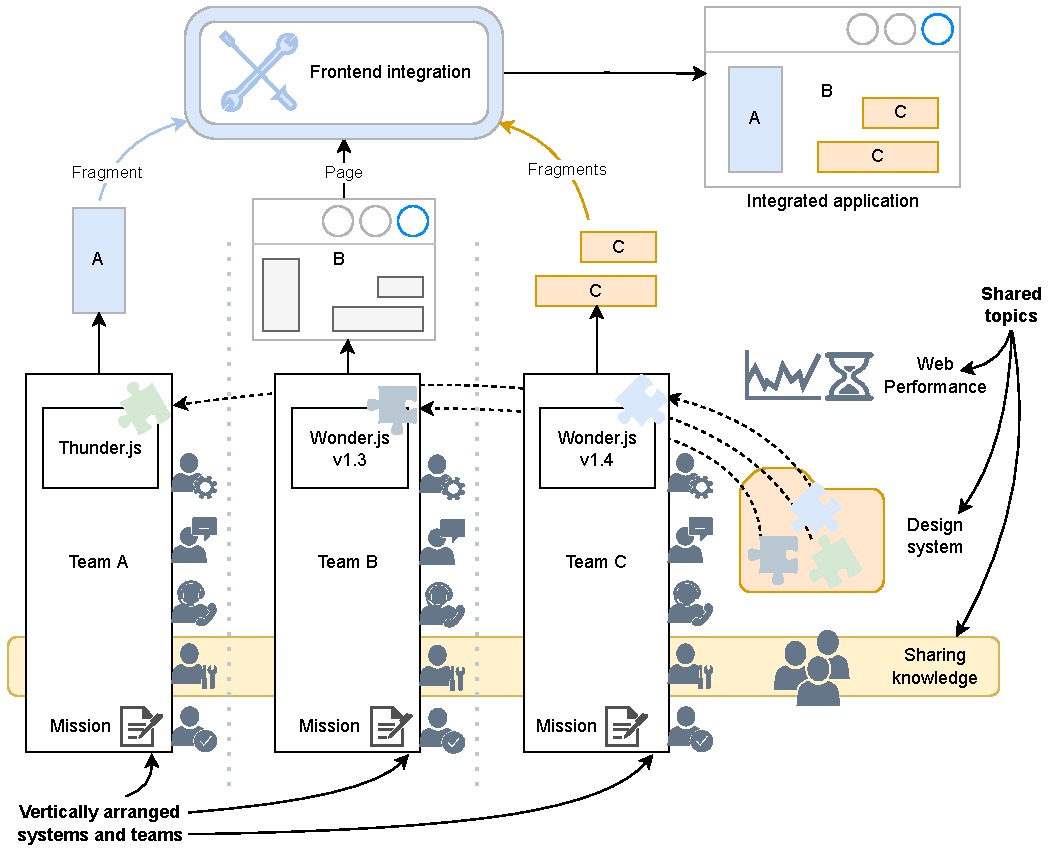
\includegraphics[width=1\textwidth]{img/MicroFrontendBigPicture}}\\
		\source{\cite[Eigene Darstellung in Anlehnung an][5]{Geers2020}} % Quelle
		\label{fig:MicroFrontendBigPicture}
	\end{minipage}
\end{figure}

Es ist zu sehen, wie die einzelnen Microfrontends verschiedener, vertikal organisierter Teams zu einer zusammenhängenden Lösung zusammengefügt werden. Die vertikale Trennung nach Domänen, realisiert mit einem Team pro Domäne, ergänzt sich mit dem horizontalen Teilen von Wissen, Design- und Architekturentscheidungen. Auch können verschiedene Technologien je Team eingesetzt werden, was die Teams unabhängiger voneinander agieren lässt. Die Stakeholder der Domäne sind ebenfalls mit in den Entwicklungsprozess integriert, was das direkte Erstellen von Lösungen, passend zu den Anforderungen, ermöglicht.

\subsection{Portalapplikationen}\label{sec:Portalapplikationen}

In diesem Kapitel wird das Konzept von Portalapplikationen erklärt. Portalapplikationen können in verschiedenen Formen realisiert werden. Im einfachsten Fall durch Hyperlinks, welche im nachfolgenden \cref{sec:PortalapplikationenHyperlinks} vorgestellt werden. Ebenfalls ist die Realisierung einer Portalshell mit Querschnittsfunktionen möglich, welche im darauffolgenden Abschnitt erläutert wird.

Eine Portalapplikation stellt die übergeordnete Webseite dar, welche die einzelnen Microfrontends miteinander verbindet.\footnote{\cite[vgl.][121]{Geers2020}} Dies kann auf unterschiedliche Arten realisiert werden, von denen zwei nachfolgend erläutert werden.

\subsubsection{Portalapplikationen durch Hyperlinks}\label{sec:PortalapplikationenHyperlinks}

Portalapplikationen können bereits durch Verlinkungen realisiert werden. In der nachfolgenden \cref{fig:LinksMicroFrontends} ist dies am Beispiel von Google Maps dargestellt. Die Seite \textit{\url{https://www.google.de/maps}} bindet diverse andere Seiten des Alphabet Konzerns ein und macht diese durch Verlinkungen erreichbar.

\begin{figure}[hbt!]
	\centering
	\begin{minipage}[t]{0.5\textwidth}	
		\caption{Verlinkung anderer Webseiten}
		\frame{
\includegraphics[width=1\textwidth]{img/MFLinks}}\\ % Pfad
		\source{Screenshot von Google Maps} % Quelle
		\label{fig:LinksMicroFrontends}
	\end{minipage}
\end{figure}

Hinter jedem der im rechten Bereich der \cref{fig:LinksMicroFrontends} zu sehenden Icons ist eine weitere Seite durch Klicken zu erreichen. So führt der Klick auf das YouTube Icon den Nutzer zu \textit{\url{https://www.youtube.com/}}. Die bisherige Seite \textit{\url{https://www.google.de/maps}} wird verlassen und der Seiteninhalt von YouTube wird dargestellt.

Der Vorteil bei dieser Art der Realisierung einer Portalapplikation besteht darin, dass Verlinkungen sehr einfach und ohne aufwändige Anpassungen einzurichten sind.

Allerdings verliert der Benutzer beim Wechseln der Webseiten seinen Fortschritt oder seine Eingaben. Ebenfalls muss Aufwand seitens der Webseitenbetreiber investiert werden, damit die verlinkten Webseiten einheitlich aussehen, um die Zusammengehörigkeit sowie das Benutzergefühl zu erhalten.\footnote{\cite[vgl.][36]{Steyer2020}}

Durch Hyperlinks kann die Produktpalette eines Unternehmens einheitlich erreichbar gemacht werden. Es können auch Informationen zu einem bestimmten Thema gesammelt werden, wie es beispielsweise bei \url{https://zeef.com/} der Fall ist. Eine Zeef-Seite zum Thema \textit{Microfrontends} ist unter folgendem Link zu finden: \href{https://micro-frontends.zeef.com/elisabeth.engel?ref=elisabeth.engel&share=ee53d51a914b4951ae5c94ece97642fc}{\nolinkurl{micro-frontends.zeef.com}}.\footnote{\cite[vgl.][]{Engel2021}}

\subsubsection{Portalshell}\label{sec:PortalapplikationenPortalshell}

Wenn das Wechseln zwischen verschiedenen Frontends nicht sichtbar geschehen soll, so muss eine Portalshell (engl. \textit{Application Shell}) gewählt werden. Eine Portalshell ist eine Portalapplikation, welche andere Microfrontends nach horizontaler Trennung einbindet. In Anhang \ref{app:Bilder} in \cref{fig:AufgabenShell} ist eine beispielhafte Portalshell dargestellt, welche das clientseitige Routing zwischen verschiedenen Microfrontends übernimmt.

Die Portalshell hat mehrere Aufgaben, welche in der nachfolgenden Liste dargestellt sind:\footnote{\cite[vgl.][45\psq]{Mezzalira2021}}

\begin{compactitem}
	\item Dynamisch Microfrontend Routen laden
	\item \textit{User state} verwalten	
	\item Fehlerbehandlung beim Laden von Microfrontends
	\item Einheitliches Logging ermöglichen
\end{compactitem}

Die Portalshell muss in der Lage sein, die Microfrontends dynamisch zu laden, damit beim Hinzufügen neuer Microfrontends keine neue Veröffentlichung der Portalshell erforderlich ist. Die Links zu den konfigurierten Microfrontends können hierfür bspw. in einer Datenbank abgelegt werden, auf welche die Portalshell zugreifen kann.\footnote{\cite[vgl.][46]{Mezzalira2021}}

Ebenfalls muss die Portalshell den \textit{User state} kennen und bei Bedarf eine Authentifizierung durchführen. Die Portalshell muss verhindern, dass ein \textit{\gls{Deeplink}} aufgerufen werden kann, wenn keine Authentifizierung und Autorisierung vorliegen. Nachdem der User authentifiziert wurde, muss die Portalshell das Aufrufen aller Microfrontends, für die er autorisiert ist, ermöglichen.\footnote{\cite[vgl.][45]{Mezzalira2021}}

Sollte ein Microfrontend nicht geladen werden können, muss die Portalshell diesen Fehler abfangen und versuchen zu beheben. Unter Umständen ist das Microfrontend mehrfach auf verschiedenen \gls{URL}s veröffentlicht und es kann auf eine andere Adresse gezeigt werden, die noch funktioniert.
Das verantwortliche Team muss informiert werden und sollte das Problem schnellstmöglich beheben. Des Weiteren muss die Portalshell das Logging von Fehlern zentral ermöglichen. Das könnte theoretisch auch jedes Microfrontend selber realisieren, doch so kann Aufwand eingespart werden und wenn diese Informationen konsolidiert an einem Ort sind, ist die Fehlersuche für die betreuenden Teams einfacher.\footnote{\cite[vgl.][46]{Mezzalira2021}}

Ebenfalls liefert die Portalshell den Microfrontends sogenannte Querschnittsaspekte. Diese können optional von den Microfrontends verwendet werden und bilden Funktionen ab, die sonst jedes Microfrontend selbstständig lösen müsste. So wird Redundanz vermieden und Einheitlichkeit gewahrt. Querschnittsaspekte sind nicht verbindlich und unterscheiden sich zwischen Portalshells, da sie von den individuellen Anforderungen abhängen.

Mögliche Querschnittsaspekte sind nachfolgend aufgelistet:\footnote{vgl. \cref{Exp1} in Anhang \ref{app:Expertengespräche}}

\begin{compactitem}
	\item User- und Mandantenverwaltung
	\item Authentifizierung \& Autorisierung
	\item Lokalisierung
	\item Konfigurationswertespeicher
\end{compactitem}

Die Portalshell verwaltet die Benutzer einer Anwendung und handhabt die Berechtigungen. Ein Benutzer wird anhand seiner Berechtigungen autorisiert. Eine Portalshell kann auch mandantenfähig sein. Das bedeutet, dass Benutzer zu einem oder mehreren Mandanten zugehörig sind. Spezielle Bereiche der Anwendung sind nur für einzelne Mandanten freigeschaltet und die Darstellung der Applikation ist für jeden Mandanten unterschiedlich. Beispielsweise entscheidet Mandant A, dass die zugehörigen Benutzer geduzt werden sollen, was die Ziel-Lokalisierung der Applikation beeinflusst.

Bei internationalen Portalapplikationen ist eine Lokalisierung empfehlenswert. So können mit einer Webseite direkt alle konfigurierten Sprachen abgebildet werden. Die Anzeigesprache ist pro User konfiguriert, sollte aber auch über das Frontend zu ändern sein, wie es beispielsweise bei einer großen Onlinehandelsplattform der Fall ist (siehe \cref{fig:PortalshellLokalisierung} in Anhang \ref{app:Bilder}). Über die Lokalisierung kann zum einen die Sprache gewechselt werden, zum anderen aber auch der Dialekt einer Sprache. Letzteres empfiehlt sich bei einer deutschsprachigen, mandantenfähigen Portalshell, abhängig davon, ob der Mandant seine Benutzer siezt oder duzt.

Ebenfalls muss die Portalshell eine Möglichkeit für Microfrontends bieten, Konfigurationen abhängig vom User und dessen Mandanten im Key-Value Format laden zu können.\footnote{\cite[vgl.][46]{Mezzalira2021}} Als Beispiel wird der Name des aktuellen Mandanten immer in den Microfrontends angezeigt, was für jeden Mandanten dementsprechend unterschiedlich konfiguriert werden und dynamisch geladen werden muss.

Mandantenfähige Portalshells mit einer Nutzerverwaltung sowie einem Rechte- und Rollenkonzept sind anspruchsvoll zu gestalten. Ebenfalls muss der Prozess der Registrierung eines neuen Microfrontends, welches sich unter Umständen je Mandant unterscheidet, abgebildet werden. Im späteren \cref{sec:PrototypischesBeispiel} wird eine beispielhafte Portalshell beschrieben, deren Prozesse im Detail erklärt werden.

\subsection{Microfrontends}\label{sec:Microfrontends}

Im \cref{sec:MicrofrontendArchitektur} wurde die übergreifende Architektur von Microfrontends erläutert. Im vorherigen \cref{sec:Portalapplikationen} anschließend dann die Portalapplikationen, als gruppierendes Konzept von Microfrontends, erläutert. In diesem Abschnitt werden nun Microfrontends einzeln erläutert. Es werden verschiedenen Techniken vorgestellt, durch welche Microfrontends zusammengesetzt und eingebunden werden können.

In den beiden nachfolgenden \crefrange{sec:ServerSideComposition}{sec:ClientSideComposition} werden die Konzepte von \textit{Server-side} und \textit{Client-side Composition} vorgestellt, welche bereits vorher in \cref{sec:MicrofrontendArchitekturTechnisch} beim Microfrontend Decision Framework angeschnitten wurden.

Danach werden in den \crefrange{sec:IFrame}{sec:ModuleFederation} verschiedene Arten der Einbindung eines Microfrontends in die Portalshell durch \textit{Client-side Composition} erläutert.

Im letzten \cref{sec:Entscheidungsvielfalt} wird eine Zusammenfassung der drei zusammengehörigen Abschnitte (\textit{Iframe}, \textit{Web Components} und \textit{Module Federation}) bezogen auf das Thema Microfrontends gegeben. Die Auswirkungen der Entscheidungsvielfalt wird anschließend mit einer generischen Betrachtungsweise durch verschiedene Entscheidungsstrukturen aufgezeigt.

\subsubsection{Server-side Composition}\label{sec:ServerSideComposition}

Bei der \textit{Server-side Composition} werden die einzelnen Fragmente der Webseite auf dem Webserver zu einer fertigen Webseite zusammengesetzt und dann als ein vollständiges Stück an den Client herausgegeben. Dies ist in der nachfolgenden \cref{fig:ServerClientSideComposition} im linken Teil dargestellt und geschieht auf dem Server durch die dort installierte Webserver-Lösung (bspw. Nginx).\footnote{\cite[vgl.][60]{Geers2020}}

\begin{figure}[hbt!]
	\centering
	\begin{minipage}[t]{1\textwidth}	
		\caption{Server- und Client-side Composition}
		\frame{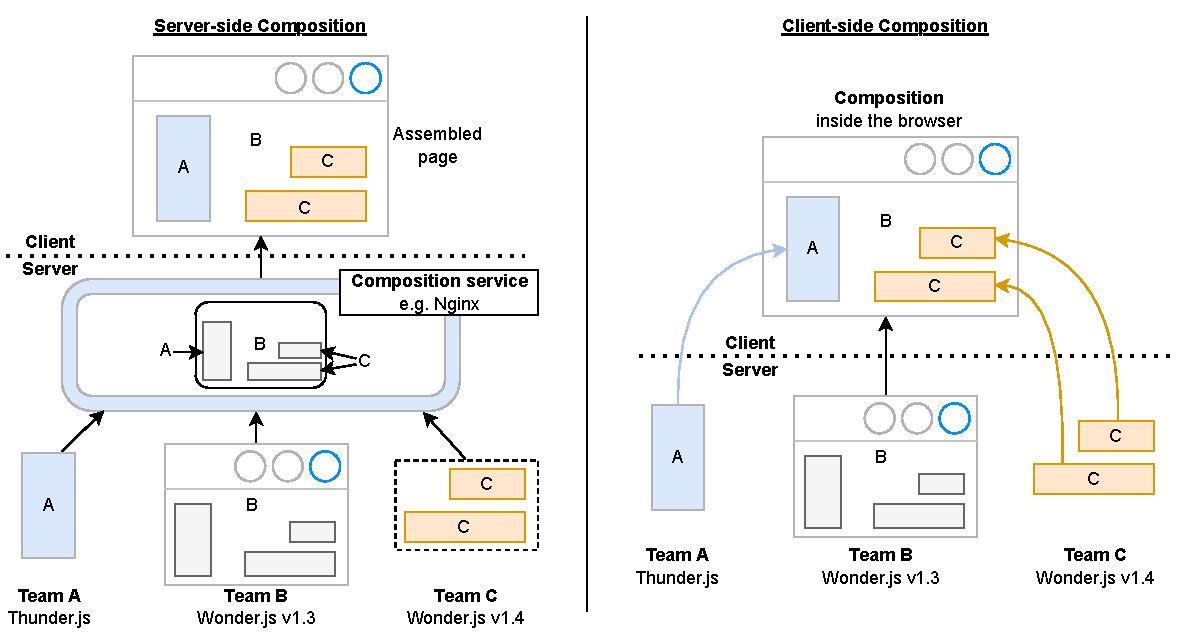
\includegraphics[width=1\textwidth]{img/ServerClientSideComposition}}\\ % Pfad
		\source{\cite[Eigene Darstellung in Anlehnung an][60,86]{Geers2020}} % Quelle
		\label{fig:ServerClientSideComposition}
	\end{minipage}
\end{figure}

Dadurch, dass die gesamte Webseite auf dem Server zusammengesetzt und als vollständige Lösung an den Nutzer ausgegeben wird, sind gute Ladezeiten zu erreichen.\footnote{\cite[vgl.][60]{Geers2020}}

Bei Nginx, einer Softwarelösung für unter anderem Webserver, Cache, Lastverteilung und Reverse Proxy,\footnote{\cite[vgl.][]{nginx2022}} werden die einzelnen Fragmente durch \textit{\gls{SSI}} serverseitig zusammengesetzt. Die Seite, welche später an den Client ausgegeben wird, beinhaltet noch Platzhalter. Diese werden durch \gls{SSI} mit dem Zielinhalt ersetzt. In Anhang \ref{app:Listing} unter \cref{list:SSIPlaceholder} ist ein exemplarischer Platzhalter dargestellt.

Die Platzhalter beinhalten den Pfad zum Code, durch welchen sie ersetzt werden sollen. Alle Platzhalter, die sich auf der auszugebenden Seite befinden, werden anschließend durch den referenzierten Code ersetzt. In der \cref{fig:SSCNginxSSI} in Anhang \ref{app:Bilder} ist ein Sequenzdiagramm dargestellt, welches die einzelnen Schritte im Detail darstellt.

\textit{Server-side Composition} bietet Vorteile durch schnelle Performance, weil der Browser direkt eine fertig zusammengesetzte Webseite geliefert bekommt. Ebenfalls ist \gls{SSI} als Technologie bewährt und \textit{Server-side Composition} ist suchmaschinenfreundlich.\footnote{\cite[vgl.][82\psq]{Geers2020}}

Die Nachteile von \textit{Server-side Composition} kommen vor allem bei großen, dynamischen Anwendungen zu Tage. Es dauert, bis alle Teile der großen Anwendung gerendert und zum Client übertragen werden. Eine Mischung von \textit{Server-} und \textit{Client-side Composition} könnte helfen, die Ladezeit zu verbessern. Ebenfalls wirken Server-side Applikationen nicht sehr interaktiv auf den Anwender. Programmteile die schnell reagieren und auf Nutzereingaben interagieren müssen, sollten für verringerte Ladezeiten clientseitig zusammengesetzt werden.\footnote{\cite[vgl.][83]{Geers2020}}

\textit{Server-side Composition} ist für den weiteren Verlauf der \dokumententyp{}
 nicht von Relevanz und wurde nur für die Gegenüberstellung zu \textit{Client-side Composition} genutzt, welche im nachfolgenden \cref{sec:ClientSideComposition} erklärt wird.

\subsubsection{Client-side Composition}\label{sec:ClientSideComposition}

Bei der \textit{Client-side Composition} werden die Fragmente einzeln heruntergeladen und erst beim Client im Browser zusammengesetzt. Auch dieser Vorgang ist in der vorherigen \cref{fig:ServerClientSideComposition} dargestellt.

Im Gegensatz zu \textit{Server-side Composition} werden bei der \textit{Client-side Composition} die einzelnen Fragmente im Browser des Client generiert und zusammengesetzt. Lösungen dafür sind beispielsweise die gängigen Javascript-Frontend-Frameworks \textit{Angular}, \textit{Vue.js} oder \textit{React}.

Je nach Art der Zusammensetzung können die Fragmente auch auf unterschiedlichen Technologien beruhen. So kann Fragment A auf einer neueren Version des Frameworks beruhen, welches die Fragmente zusammensetzt. Fragment B kann sogar auf einer ganz anderen Technologie beruhen, solange es die benötigten Referenzen und Bibliotheken eigenständig mitbringt.

\textit{Client-side Composition} bietet sich bei interaktiven Anwendungen an, wie beispielsweise einer Web Applikation zum Erstellen der Steuererklärung. Eine statische Anwendung kann besser serverseitig zusammengesetzt und mit einzelnen clientseitigen Komponenten versehen werden, bei denen vorwiegend dynamischer Inhalt angezeigt wird.\newline
Ebenfalls ist es durch Iframes und Web Components möglich, eine starke, technische Isolierung der \gls{UI} zu erzielen.\footnote{\cite[vgl.][97]{Geers2020}} Dadurch können sich Fragmente verschiedener Teams in den Stylings nicht überschreiben, was bei \textit{Server-side Composition} nur durch strikte Konventionen, wie beispielsweise Prefixe für CSS-Klassen und Namespaces, möglich ist.\footnote{\cite[vgl.][83]{Geers2020}}

In den nachfolgenden Abschnitten werden drei Arten der clientseitigen Einbindung eines Microfrontends vorgestellt.

\subsubsection{Iframe}\label{sec:IFrame}

Das \textit{Inline Frame} (nachfolgend Iframe) ist ein \gls{HTML} Element, durch welches andere HTML-Webseiten in die bestehende Webseite eingebunden werden können. Es wird von allen aktuellen Browsern unterstützt.\footnote{\cite[vgl.][]{MDNWebDocs2021a}}
Im nachfolgenden \cref{list:iframe} ist ein beispielhaftes Iframe zu sehen, über welches die Webseite der \gls{FHDW} eingebunden wird.

\begin{figure}[bht]
	\begin{lstlisting}[caption=Exemplarische Einbindung einer Webseite über das Iframe-Element, label=list:iframe]
		<iframe id="iframeId" src="https://fhdw.de/" name="FHDW-Webseite" 
		width="500" height="200" style="border: none"></iframe>
	\end{lstlisting}
	\footnoterule{}
	\footnotesize{\textbf{Quelle:} Eigene Darstellung}
\end{figure}

Dem Iframe Element wird über den \texttt{src}-Parameter die \gls{URL} der einzubindenden Webseite mitgegeben. Über die Parameter \texttt{width} und \texttt{height} können Anpassungen an der Breite und Höhe des Elements, in dem die eingebundene Webseite angezeigt wird, getätigt werden. Dies ist erforderlich, sollte die Standardauflösung von 300px x 150px nicht ausreichen.\footnote{\cite[vgl.][]{MDNWebDocs2021a}}

Ebenfalls kann über den \texttt{style}-Parameter eigener \gls{CSS} Code auf das \gls{HTML}-Element angewendet werden. Durch diesen Parameter kann unter anderem der standardmäßige Rahmen ausgeblendet werden, um die Einbindung einer externen Ressource für den Anwender weniger offensichtlich zu machen.

Ein Iframe kann, wenn es in eine andere Anwendung eingebunden wird, diese nicht durch Styles beeinflussen. Die Kapselung der UI ist dementsprechend hoch gegenüber anderen Microfrontends.

Das Iframe eignet sich als schnelle Art der Einbindung mit hoher Kapselung des Inhalts gegen andere Microfrontends. Iframes haben eine schlechte Performance, wenn viele von ihnen eingebunden werden. Jedes Iframe erstellt einen neuen Browserkontext, welcher Rechen- und Speicherintensiv ist. Ebenfalls sind Iframes für Screenreader und Suchmaschinen nicht gut zu erreichen, was in geringer Suchmaschinenoptimierung und geringer Barrierefreiheit resultiert.\footnote{\cite[vgl.][35]{Geers2020}}

\subsubsection{Web Components}\label{sec:Webcomponents}

Web Components bestehen aus drei Technologien: \textit{Shadow DOM}, \textit{Custom Elements} und \textit{HTML Templates}.\footnote{\cite[vgl.][]{MDNWebDocs2022a}}

Durch das \textit{Shadow \gls{DOM}} wird einem \gls{HTML}-Element ein eigener, sogenannter Shadow, \gls{DOM} Tree gehängt. Dieser Tree wird vom Browser separat und unabhängig vom Main \gls{DOM} gerendert. Das separate Rendering der beiden \gls{DOM}s hat zur Folge, dass diese voneinander abgekapselt agieren und sich nicht gegenseitig beeinflussen können. So haben \gls{CSS}-Konfigurationen innerhalb des Shadow \gls{DOM} Trees keine Auswirkungen auf Elemente außerhalb des eigenen Trees. Dadurch wird vermieden, dass eingebundener Code die einbindende Webseite beeinflusst und zugleich nicht von \gls{CSS}-Konfigurationen der einbindenden Webseite beeinflusst wird.

Die Elemente im Shadow \gls{DOM} zu Kapseln hat Vor- und Nachteile. Durch den eigenen \gls{DOM} ist die Isolierung des Codes gegenüber anderen Microfrontends, wie bei Iframes auch, sehr stark. Ebenfalls können globale Styles die Web Component nicht beeinflussen, was bei legacy Anwendungen ein Vorteil ist. 
Auf der anderen Seite wird Shadow \gls{DOM} in alten Browsern nicht unterstützt und die Kapselung der Styles ist mit einigen Design Frameworks nicht kompatibel. Beispiele für inkompatible Frameworks sind Twitter Bootstrap oder Angular Material.\footnote{\cite[vgl.][96]{Geers2020}}

Für wiederverwendbaren \gls{HTML} Code werden \textit{\gls{HTML} Templates} verwendet. Ein Template wird über den \gls{HTML}-Tag \texttt{template} definiert und der Inhalt dessen bleibt beim Laden der Seite erst einmal verborgen. Das Template kann später je nach Bedarf ein oder mehrere Male über \gls{JS} nachgeladen werden. Ein beispielhaftes Template ist in Anhang \ref{app:Listing} in \cref{list:HTMLTemplate} dargestellt.

Durch \textit{Custom Elements} wird ermöglicht, dass neben den vordefinierten \gls{HTML} Tags noch weitere, individuelle \gls{HTML} Tags der Webseite hinzugefügt werden können. Der Inhalt eines Templates kann zu einem \textit{Custom Element} Tag hinzugewiesen werden. Die dahinterliegende \textit{Custom Elements} API rendert aus dem individuellen \gls{HTML} Tag dann anschließend den definierten Inhalt.\footnote{\cite[vgl.][]{Rauber2021}}

Web Components sind ein anerkannter Webstandard, der direkt mit der Browser \gls{API} interagieren kann. Die starke Isolation des Inhaltes bei Bedarf sorgt für eine robuste Einbindung.\footnote{\cite[vgl.][96\psq]{Geers2020}} Dafür benötigen Web Components auch \gls{JS} clientseitig und unterstützen kein serverseitiges Rendering. Dies ist zwar über Umwege realisierbar, aber nicht der vorgesehene Standard, was bei Anforderungen an geringe initiale Ladezeiten von Nachteil ist.\footnote{\cite[vgl.][97\psq]{Geers2020}}

\subsubsection{Webpack Module Federation}\label{sec:ModuleFederation}

Webpack ist ein OpenSource Modulbundler, welcher Module und deren Abhängigkeiten in statische Pakete umwandelt. Das Frontend Framework Angular benutzt Webpack zum Transpilieren, Kompilieren und Veröffentlichen von Quellcode.\footnote{\cite[vgl.][133]{Clow2018}}

Mit der Major Version 5 von Webpack, welche im Oktober 2020 offiziell erschienen ist, wurde ein neues Feature namens \textit{Module Federation} vorgestellt.\footnote{\cite[vgl.][]{Webpack2020a}} Durch Module Federation sind zwei neue Plugins hinzugekommen: Das \textit{ContainerPlugin} und das \textit{ContainerReferencePlugin}.

Das \textit{ContainerPlugin} ermöglicht asynchronen Zugriff auf Module, welche in einem Container zur Verfügung gestellt werden. Das \textit{ContainerReferencePlugin} ermöglicht Referenzen zu anderen, entfernten Containern, wodurch Module aus diesen entfernten Containern importiert und genutzt werden können.\footnote{\cite[vgl.][]{Webpack2020b}}

Die Entwickler von Webpack beschreiben zwei Anwendungsfälle. Mit dem Ersten können klassische Microfrontend Applikationen realisiert werden. So sind alle Unterseiten einer Webseite als eigene Container veröffentlicht, welche ihren Inhalt als Modul bereitstellen. Die zentrale Seite, beispielsweise die Startseite der Webseite mit Navigationseinträgen im Header- und Seitenbereich, referenziert als Application Shell durch das \textit{ContainerReferencePlugin} alle Unterseiten und bindet deren Content ein. Des Weiteren stellt die Application Shell gängige Bibliotheken bereit, auf die die Unterseiten zugreifen können. Da die Bibliotheken geteilt werden ist sichergestellt, dass diese nur einmal geladen werden.\footnote{\cite[vgl.][]{Webpack2020b}}

Das unabhängige Einbinden der Seiten hat zur Folge, dass die Unterseiten alle einzeln neu veröffentlicht werden können, wenn neuer Inhalt für eine neue Version bereit steht. Die aufrufende Seite muss nur dann neu veröffentlicht werden, wenn Änderungen an den Links vorgenommen werden. Wird lediglich der Inhalt der Unterseiten geändert, ist keine neue Veröffentlichung der Hauptseite erforderlich.\footnote{\cite[vgl.][]{Webpack2020b}}

Beim zweiten Anwendungsfall wird eine Komponentenbibliothek, bspw. ein \gls{SDK}, zum Einbinden zur Verfügung gestellt. Alle Apps, die mit diesem \gls{SDK} arbeiten, integrieren es mittels Module Federation in ihre Applikation. Wenn eine neue Version des \gls{SDK}s veröffentlicht werden soll, muss nur das Modul des \textit{ContainerPlugins} neu veröffentlicht werden und nicht jede einbindende App.\footnote{\cite[vgl.][]{Webpack2020b}}

\textbf{Module Federation in Angular}\\
Webpack ist der Modulbundler für Angular. Seit Angular Version 11 wird Webpack in der Major Version 5 unterstützt. Dadurch ist mit Module Federation ein weiterer Weg zur Einbindung eines Microfrontends in eine Portalshell hinzugekommen. Module Federation ermöglicht es, Programmteile zu referenzieren die zur Compilezeit noch nicht bekannt sind. Ebenfalls können sich verschiedene Microfrontends Bibliotheken teilen, sodass diese nur einmal vom Client geladen werden müssen.\footnote{\cite[vgl.][39]{Steyer2020}}

Damit eine Applikation mittels Module Federation eingebunden werden kann, müssen auf beiden Seiten Konfigurationen vorgenommen werden. In der nachfolgenden \cref{fig:ModuleFederation} sind die notwendigen vier Schritte zur Einbindung dargestellt.

\begin{figure}[hbt!]
	\centering
	\begin{minipage}[t]{0.64\textwidth}	
		\caption{Notwendige Konfigurationen für Module Federation}
		\frame{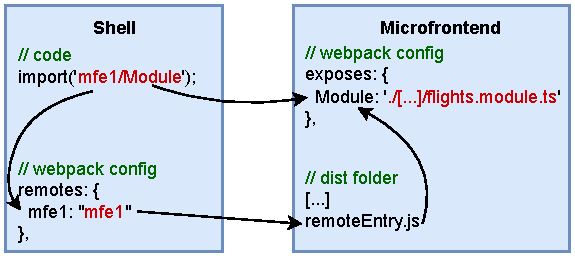
\includegraphics[width=1\textwidth]{img/ModuleFederationConfig.pdf}}\\ % Pfad
		\source{\cite[Eigene Darstellung in Anlehnung an][]{Steyer2020a}} % Quelle
		\label{fig:ModuleFederation}
	\end{minipage}
\end{figure}

Jede Applikation, die Module Federation einsetzt, muss über eine \texttt{webpack.config.js}-Datei verfügen. Über diese Datei wird Webpack konfiguriert und die Module der Applikation aufgelistet, welche exportiert und importiert werden sollen. Die Portalshell referenziert ein entferntes Modul. Dieses Modul wird von einem Microfrontend exportiert und in die \texttt{remoteEntry.js}-Datei im \textit{dist}-Ordner von Webpack geladen. Der Pfad zu diesem Ordner ist in der Konfiguration der Shell hinterlegt.

In \cref{lst:ModuleFederationWebpackRemote} in Anhang \ref{app:Listing} ist der relevante Teil einer \texttt{webpack.config.js}-Datei für eine RemoteApp zu sehen. Die RemoteApp veröffentlicht in der \texttt{remoteEntry.js}-Datei das Angular Distant-Modul mit dem Namen \textit{microapp}.

In \cref{lst:ModuleFederationWebpackShell} in Anhang \ref{app:Listing} ist der dazugehörige relevante Teil einer \texttt{webpack.config.js}-Datei einer Shell zu sehen. 
Die Shell bindet das RemoteModul \textit{microapp} ein, welches unter \texttt{microapp@http://localhost:3000/remoteEntry.js} zu finden ist. Das @-Zeichen trennt dabei den Namen des Microfrontends von der \gls{URL} des Microfrontends.

Ebenfalls sind in der Konfiguration der Shell die Bibliotheken zu sehen, welche für die RemoteApps zur Verfügung gestellt werden. Im Beispiel von \cref{lst:ModuleFederationWebpackShell} in Anhang \ref{app:Listing} werden die vier gängigen Angular Bibliotheken \textit{@angular/core}, \textit{@angular/common}, \textit{@angular/common/http} und \textit{@angular/router} zur Verfügung gestellt. Das Microfrontend hat die gleichen Bibliotheken als geteilt konfiguriert und greift auf die Bibliotheken der Shell zurück, anstatt sie selbst mitzubringen.

Damit die Shell mit dem Microfrontend Daten austauschen kann, muss in den Konfigurationsdateien beider Seiten ein \texttt{SharedMapping}-Objekt referenziert werden. 
Dort kann eine individuelle Angular Library\footnote{\cite[Für weitere Informationen siehe][]{Angular2022h}} eingebunden werden, welche von der Shell befüllt und vom Microfrontend konsumiert wird.\footnote{\cite[vgl.][]{Steyer2021d}}

\textbf{Module Federation mit Web Components}\\
Mit Module Federation ist es ebenfalls möglich, neben Angular Modulen und Komponenten, auch Web Components zu Teilen. Dies ist dann sinnvoll, wenn die einbindende Shell über eine andere Framework Version als das Microfrontend verfügt.

Dafür muss das Microfrontend in der \texttt{app.module.ts} die zu exportierende Angular Komponente als \texttt{customElement} definieren, analog wie in \cref{sec:Webcomponents} beschrieben. In der Webpack Konfiguration muss anstelle des Modules die \texttt{bootstrap.ts} veröffentlicht werden.
Statt eines Modules wie bei der vorherigen Variante, lädt die Portalshell ein Script von dem RemoteEntry.\footnote{\cite[vgl.][]{Steyer2021a}}

Durch das Einbinden einer Web Component können Microfrontends einer anderen Angular Major Version geladen und geteilt werden. Ebenfalls können Web Components eingebunden werden, die in einem anderen Web Frontend Framework erstellt wurden (bspw. in React). In  \cref{fig:ModuleFederationSchnittmengenFrameworks} in Anhang \ref{app:Bilder} sind Schnittmengen von vier Microfrontends mit einer Shell skizziert. Bibliotheken mit gleicher Major Versionsnummern können geteilt werden, wie es bei \gls{MFE2} und \gls{MFE3} der Fall ist. Module Federation wählt automatisch die Bibliothek mit der höheren Minor Version und teilt sie zwischen Shell und Microfrontend. Microfrontends mit anderen Web Frameworks, wie das React \gls{MFE4} in der Abbildung, müssen vollständig zum Client übertragen werden.
 
\subsubsection{Auswirkungen der Entscheidungsvielfalt}\label{sec:Entscheidungsvielfalt}

In diesem abschließenden Abschnitt sollen die Auswirkungen der großen Entscheidungsvielfalt beim Thema Microfrontends verdeutlicht werden. In den vorherigen Abschnitten wurde auf die Architektur von Microfrontends, Portalapplikationen und verschiedene Microfrontend-Varianten eingegangen. Je nachdem, welche Entscheidungen Softwarearchitekten für die Applikationen treffen, ergeben sich unterschiedliche Konsequenzen für die verwendeten Technologien.

Die Softwarearchitekten, welche eine Microfrontend-Architektur auswählen, müssen verschiedene Entscheidungen treffen. Diverse Lösungsarten für Komposition und Routing sind in der nachfolgenden \cref{fig:TrennungRoutingStrategien} dargestellt.

\newpage
\begin{figure}[hbt!]
	\centering
	\begin{minipage}[t]{0.8\textwidth}	
		\caption{Weiterleitung und Zusammensetzung von Microfrontends}
		\frame{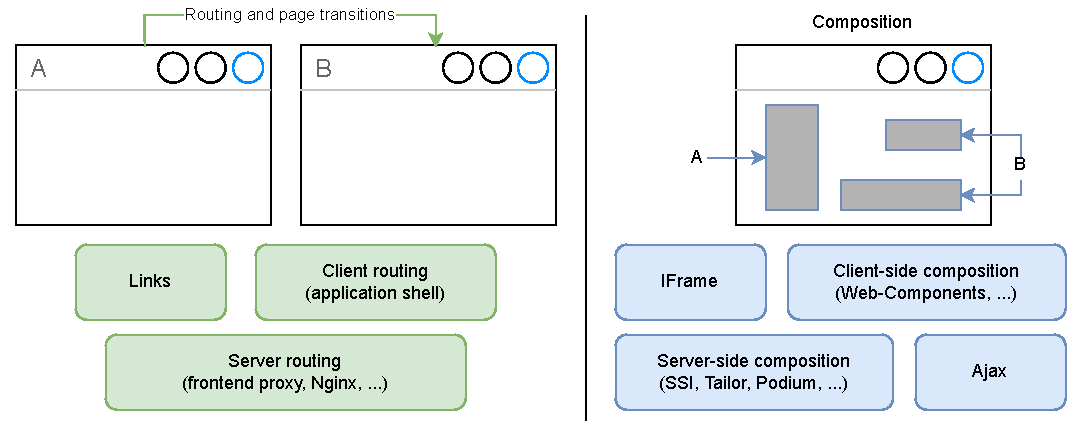
\includegraphics[width=1\textwidth]{img/TrennungRoutingStrategien}}\\ % Pfad
		\source{\cite[Eigene Darstellung in Anlehnung an][5]{Geers2020}} % Quelle
		\label{fig:TrennungRoutingStrategien}
	\end{minipage}
\end{figure}

Wenn durch das Routing die Seite wechselt oder sichtbar neu geladen werden muss, wird nachfolgend von \textit{hartem Routing} gesprochen. Das Gegenstück dazu ist \textit{softes Routing}, bei welchem die Seiteninhalte dynamisch ohne Übergang ausgetauscht werden. Das Routing bestimmt das Benutzererlebnis und kann mit hartem Routing durch Links realisiert werden, oder aber auch client- oder serverseitig geschehen. Bei den gängigen Web Fontend Frameworks sind Lösungen für softes Routing enthalten, wie beispielsweise der \textit{Angular Router} bei Angular. Softes Routing ist für den Benutzerkomfort zu empfehlen, wohingegen ein hartes Routing durch Links den Wechsel in eine andere Webseite der Produktpalette eines Unternehmens signalisiert.

Das Einbinden der Microfrontends in eine Shell kann durch verschiedene Techniken realisiert werden. Alle haben Vor- und Nachteile. Es muss anhand des gegebenen Anwendungsfalles jeweils individuell entschieden werden, welche dieser Techniken zum Einsatz kommen.

Ein möglicher Entscheidungsbaum ist nachfolgend in der \cref{fig:EntscheidungsbaumArchitektur} dargestellt. Die Abbildung bietet anhand der Anforderungen eine Entscheidungshilfe bei der Auswahl der Kompositionstechnik des Frontends.

\newpage
\begin{figure}[hbt!]
	\centering
	\begin{minipage}[t]{0.8\textwidth}	
		\caption{Microfrontend-Architektur Entscheidungsbaum nach Geers}
		\frame{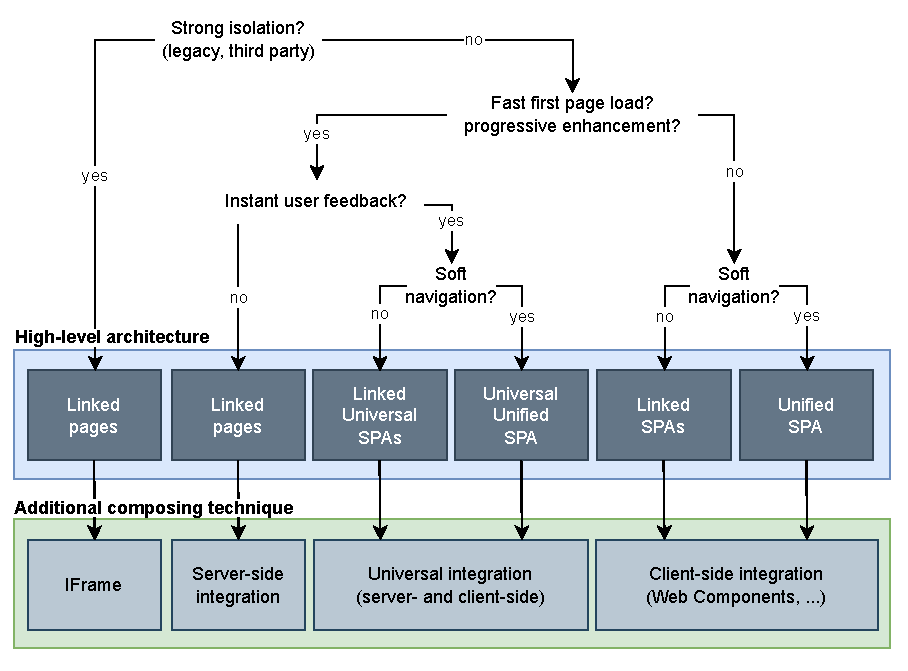
\includegraphics[width=1\textwidth]{img/EntscheidungsbaumArchitektur}}\\ % Pfad
		\source{\cite[Eigene Darstellung in Anlehnung an][166]{Geers2020}} % Quelle
		\label{fig:EntscheidungsbaumArchitektur}
	\end{minipage}
\end{figure}

Die Entscheidung zur Art der Einbindung hängt davon ab, welche Isolation gewünscht ist, wie sich die App beim Navigieren verhalten soll und ob Wert auf initiale Ladezeiten gelegt wird.

Andere Autoren haben ähnliche Entscheidungsbäume veröffentlicht. So hat beispielsweise Manfred Steyer 2018 einen Leitfaden zu Microfrontends anhängig von Architekturzielen veröffentlicht (siehe \cref{fig:EntscheidungsbaumArchitekturMF} in Anhang \ref{app:Bilder}), welcher allerdings Module Federation noch nicht beinhaltet.\footnote{\cite[vgl.][]{Steyer2018}}

%!TEX root = ../Thesis.tex
\section{Prototypisches Beispiel in Angular}\label{sec:PrototypischesBeispiel}

In diesem Kapitel wird ein prototypisches Beispiel beschrieben, auf welches sich die im nachfolgenden \cref{sec:Evaluierung} stattfindende Evaluierung beziehen wird. Das Ergebnis der Evaluierung wird im darauffolgenden \cref{sec:Implementierung} angewendet, um die Ergebnisse zu verifizieren.

Zum Verständnis des Prototypen wird in den nachfolgenden Abschnitten zunächst die Architektur in einer Schichtenansicht präsentiert und anschließend detaillierter auf die Portalshell sowie die eingebundenen Microfrontends eingegangen. Zuletzt werden in \cref{sec:PrototypAnforderungen} die Anforderungen der Microfrontends für die Einbindung in die Portalshell konkret benannt, damit diese in der Evaluierung im darauffolgendem Kapitel berücksichtigt werden können.

\textbf{Szenario des Beispieles}\\
Bei der nachfolgend beschriebenen Beispielapplikation handelt es sich um eine Portalshell, welche im \gls{B2B}-Kontext verwendet wird. Firmenkunden wird Zugang zu der Portalshell gewährt und diese können über die Softwarelösung ihre Backoffice Tätigkeiten erledigen. Die Portalshell ist mandantenfähig, denn jeder \gls{B2B} Kunde soll individuell konfigurierte Microfrontends nutzen können. 

Damit die Portalshell nicht bei jedem hinzugefügten Microfrontend jedes Mandanten neu veröffentlicht werden muss, ist das Anzeigen der Microfrontends dynamisch gelöst. Es werden von den Usern die individuellen Konfigurationen und Anordnungen der Microfrontends zur Laufzeit geladen. Als Beispiel möchte Kunde A auf der Startseite ein Microfrontend zum Ticketmanagement angezeigt bekommen. Kunde B hingegen benötigt auf der Startseite zwei konfigurierte \gls{KPI}s sowie ein Microfrontend zur Suche auf dem eigenen Fileshare.

Die Portalshell bietet den Microfrontends, welche auch teilweise vom \gls{B2B} Kunden selber entwickelt werden, die Möglichkeit auf Querschnittsaspekte des Portals zuzugreifen. Darunter fallen beispielsweise Logging, Lokalisierung, Benutzer- und Mandanteninformationen, Autorisierung und das Laden von Konfigurationswerten. Die Portalshell wird von mandantenunabhängigen Administratoren übergreifend verwaltet. Sie können neue Microfrontends registrieren, User anlegen und diese zu Mandanten zuweisen sowie einen First-Level-Support stellen. Die Administratoren sind ebenfalls für den Betrieb der Portalshell zuständig und Hosten diese in Azure.

In den nachfolgenden Abschnitten wird die Architektur sowie Details zu drei prototypischen Microfrontends für einen Mandanten im Detail präsentiert.

\subsection{Architekturübersicht}\label{sec:PrototypArchitekturdiagramm}

In der nachfolgenden Abbildung \cref{fig:ArchitekturBsp} ist die beispielhafte Microfrontendarchitektur dargestellt und in die Schichten Frontend, Backend und Datenbank getrennt. 

\begin{figure}[hbt!]
	\centering
	\begin{minipage}[t]{0.8\textwidth}	
		\caption{Beispielapplikation Microfrontend-Architektur}
		\frame{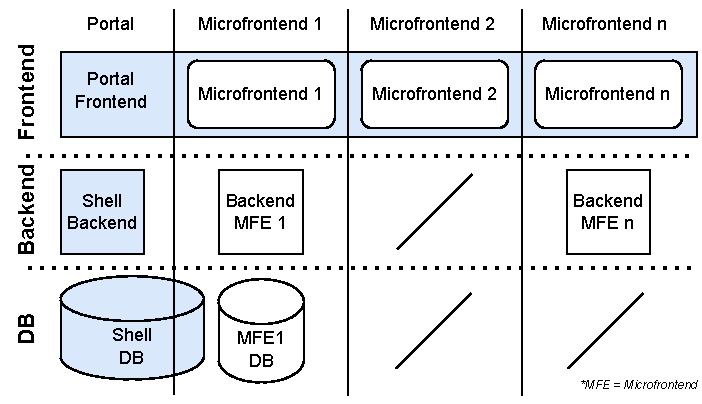
\includegraphics[width=1\textwidth, page=1]{img/Beispielapplikation_Diagramm}}\\ % Pfad
		\source{Eigene Darstellung} % Quelle
		\label{fig:ArchitekturBsp}
	\end{minipage}
\end{figure}

Die Applikation besteht aus einer Portalshell, zu welcher ein Frontend, ein Backend sowie eine Datenbank gehört. In das Frontend der Portalshell sind mehrere Microfrontends eingebunden, welche entweder aus einem Frontend mit einem eigenen Backend sowie einer eigenen Datenbank bestehen (siehe \gls{MFE1}), nur aus einem Frontend bestehen (siehe \gls{MFE2}) oder aus einem Frontend und einem Backend bestehen (siehe Microfrontend n).

Das Backend der Portalshell sowie das Backend des \gls{MFE1} greifen jeweils auf die Datenbank der Portalshell zu (siehe nachfolgende \cref{fig:SolutionarchitekturBsp}). Die Portalshell verwaltet die Nutzer und deren Berechtigungen. Sie stellt Schnittstellen bereit, damit Microfrontends die Nutzerinformationen bei Bedarf konsumieren können.

\newpage
\begin{figure}[hbt]
	\centering
	\begin{minipage}[t]{0.6\textwidth}	
		\caption{Beispielapplikation Solutionarchitektur}
		\frame{\includegraphics[width=1\textwidth,page=2]{img/Beispielapplikation_Diagramm}}\\ % Pfad
		\source{Eigene Darstellung} % Quelle
		\label{fig:SolutionarchitekturBsp}
	\end{minipage}
\end{figure}

Die Portalapplikation verfügt über ein Rollenkonzept. Die Rollen werden für jeden User pro Microfrontend vergeben. Das Microfrontend 1 fragt die \gls{DB} der Portalshell nach der Rolle des aktuellen Users ab, weil es diese Information zum Anzeigen der Inhalte benötigt. Bei Microfrontend n und \gls{MFE2} haben alle Benutzer die gleichen Rechte, weswegen Abfragen der Rollen nicht nötig sind. Das \gls{MFE2} fragt in regelmäßigen Abständen eine öffentliche \gls{API} an und zeigt die Ergebnisse der Anfrage aufbereitet im Frontend an.

\subsection{Portalapplikation}\label{sec:PrototypPortalapplikation}

Die Portalapplikation basiert auf dem Angular Framework und bietet, wie in \cref{sec:Portalapplikationen} beschrieben, einige Querschnittsaspekte.

So ist Authentifizierung sowie die generelle Benutzerverwaltung über das Portal abgedeckt. Für Benutzer muss, bevor sie sich im Portal anmelden können, ein Account zum Einloggen sowie eine dazugehörige Rollenzuweisung angelegt werden. Es sind zwei Rollen verfügbar, welche in der \cref{tab:RollenPortalapplikation} in Anhang \ref{app:Tabellen} mit ihrer jeweiligen Funktion dargestellt sind.

Eine Rollenzuweisung stellt die Verbindung zwischen einem Benutzer und einem Mandanten her. Ein Benutzer kann in mehreren Mandanten jeweils eine Rolle zugewiesen bekommen. Eine Übersicht der zusammenhängenden Elemente in der Portalapplikation ist in der nachfolgenden \cref{fig:NutzerMandantenDashboard} zu sehen.

\begin{figure}[hbt!]
	\begin{minipage}[t]{1\textwidth}	
		\caption{Übersicht der Elemente der Portalshell}
		\frame{\includegraphics[width=1\textwidth, page=4]{img/Beispielapplikation_Diagramm}}\\ % Pfad
		\source{Eigene Darstellung} % Quelle
		\label{fig:NutzerMandantenDashboard}
	\end{minipage}
\end{figure}

In dem Portal können Microfrontends dynamisch eingebunden werden. Es gibt eine Oberfläche, auf der Administratoren des Portals neue Microfrontends konfigurieren können. Zu jedem Microfrontend wird ebenfalls die Konfiguration der Parameter des Microfrontends gespeichert. Microfrontends können anschließend instanziiert werden, indem sie einem Mandanten zugewiesen und die Parameter-Konfigurationen auf die Werte des Mandanten gesetzt werden. So können die Microfrontends dynamisch für verschiedene Mandanten gleichzeitig genutzt werden. Eine Übersicht der Elemente mit beispielhaften Ausprägungen ist zur besseren Verständlichkeit in Anhang \ref{app:Bilder} in \cref{fig:PortalapplikationElementeKonkret} dargestellt.

Ein Dashboard bezeichnet eine für einen Mandanten individuell konfigurierte Anordnung von Microfrontendinstanzen, auf die Benutzer eines Mandanten zugreifen können. Die einzelnen Microfrontendinstanzen können für den eingebunden Mandanten individuell konfiguriert sein. Liegt keine Konfiguration vor, wird entweder auf einen Standardwert des Microfrontend-Templates zurückgegriffen oder ganz auf Konfiguration verzichtet.

Die Nutzer eines Mandanten können sich die eingebundenen Microfrontendinstanzen individuell auf dem Dashboard konfigurieren, wie es zum Beispiel auch bei Azure Dashboards der Fall ist.\footnote{\cite[vgl.][]{Microsoft2021a}} Die Portalshell stellt Dialoge zum Registrieren und Verwalten von Dashboards für einen Mandanten zur Verfügung.

Damit die Portalapplikation sowie die eingebundenen Microfrontends integriert werden können und dem gleichen Design folgen, wird ein \gls{SDK} zur Verfügung gestellt. Dieses beinhaltet Formularelemente, wie beispielsweise Buttons, interaktive Textboxen oder Dropdownlisten. Diese Formularelemente sind einheitlich gestylt und können miteinander interagieren, um clientseitige Validierung zu ermöglichen.

Ebenfalls sorgt die Portalshell für Fehlerbehandlung, sollte ein Microfrontend in einem Dashboard nicht geladen werden können. In diesem Fall wird ein Platzhalter mit entsprechendem Text angezeigt und der Fehler protokolliert, damit das Entwicklerteam reagieren kann. Auch bietet das Portal eine Schnittstelle, damit eingebundene Microfrontends etwaige Fehler zentral protokollieren können.

\subsection{Eingebundene Microfrontends}\label{sec:PrototypMicrofrontends}

In die im vorherigen Abschnitt beschriebene Portalapplikation werden Microfrontends eingebunden. Um ein Microfrontend einbinden zu können, muss dieses vorher im Portal mit den Parametern \gls{URL}, Art der Einbindung und optionalen mandantenindividuellen Konfigurationen registriert werden. Es entsteht ein Template des Microfrontends, welches nur die Hosting-Parameter sowie die Schlüssel der Konfigurationen enthält. Die Ausprägungen der Konfigurationen werden bei der Instanziierung des Microfrontends zu einem Mandanten gesetzt. Anschließend lädt die Portalshell die Konfiguration der Microfrontendinstanz dynamisch aus der Datenbank, damit sie nicht immer bei jeder Änderung an den konfigurierten Microfrontends neu veröffentlicht werden muss.

Im Fall der in \cref{fig:ArchitekturBsp} beschriebenen Architektur handelt es sich bei \gls{MFE2} um eine Wetter-Applikation, welche regelmäßig eine Wetter-\gls{API} aufruft. Für jeden Mandanten ist der Standort als Parameter der Microfrontendinstanz konfiguriert, sodass das Wetter des Standortes angezeigt wird, an welchem der Mandant sich befindet. Exemplarisch soll für den prototypischen Mandanten das Wetter von zwei Standorten angezeigt werden, da Benutzer das Wetter an ihrem Arbeitsplatz, aber auch von ihrer Heimatstadt verfolgen können sollen. Von dem Wetter-Microfrontend werden dementsprechend zwei Instanzen mit unterschiedlichen Parametern eingebunden.

Microfrontend n ist eine Taschenrechner App, welche von allen Usern genutzt werden darf. Die Taschenrechner-App verfügt über keine Parameter und ist für alle Mandanten gleich.

Microfrontend 1 stellt eine Statistik App dar. Diese darf von allen Benutzern angezeigt werden. Normale Benutzer sehen die App mit verringertem Umfang. Nutzer mit der Administrator-Rolle sehen erweiterte Statistiken, die sonst nicht sichtbar sind. Die Statistik-App fragt die Portalapplikation an, ob der Benutzer ausreichend Rechte hat, um den Administrator-Bereich der Statistik-App einsehen zu dürfen. Dafür muss die Statistik-App Informationen über den aktuellen Benutzer kennen, wie beispielsweise seinen Namen und eine eindeutige Kennung.

Die externen Abhängigkeiten der Microfrontends sind in einer Solutionarchitektur  dargestellt, welche in Anhang \ref{app:Bilder} in \cref{fig:SolutionarchitekturBeispielapplikationKonkret} abgebildet ist.

Ein Mockup des Designs von der Portalshell mit den vier eingebundenen Microfrontendinstanzen auf einem Dashboard mit dem Namen \textit{Prototyp} ist in der nachfolgenden \cref{fig:MockupBeispiel} dargestellt. Die blauen Balken links und oben werden von der Portalshell gestellt. Links an der Seite befindet sich die Navigation, durch die zwischen Dashboards gewechselt werden kann. Oben im Header sind Informationen zum Mandanten sowie ein Icon sichtbar, auf welches der Benutzer zum Verwalten seines Profils und zum Abmelden klicken kann.

\begin{figure}[hbt!]
	\centering
	\begin{minipage}[t]{0.7\textwidth}	
		\caption{Design Mockup Dashboard \textit{Prototyp}}
		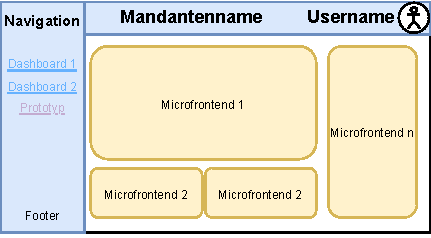
\includegraphics[width=1\textwidth]{img/MockupBeispiel}\\ % Pfad
		\source{Eigene Darstellung} % Quelle
		\label{fig:MockupBeispiel}
	\end{minipage}
\end{figure}

Der restliche in weiß dargestellte Bereich der rechteckigen Anwendung ist der Platzhalter des ausgewählten Dashboards. Die vier eingeblendeten Microfrontendinstanzen entstammen drei konfigurierten Microfrontend-Templates.

\subsection{Anforderungen an das System}\label{sec:PrototypAnforderungen}

Nach dem Definieren der Portalapplikation sowie den eingebundenen Microfrontends können konkrete Anforderungen gestellt werden, welche die Art der Einbindung erfüllen sollte.

Durch das in \cref{fig:NutzerMandantenDashboard} aufgezeigte und in \cref{sec:PrototypMicrofrontends} beschriebene Konzept der Konfigurierbarkeit der Microfrontends muss bei der Art der Einbindung eine Möglichkeit bestehen, Parameter übergeben zu können. Ansonsten wäre eine mandantenfähige Portalapplikation nicht zu realisieren.

Da die \gls{UX} das Erlebnis des Benutzers auf der Webseite beschreibt, spielt sie eine relevante Rolle. So sollten Portalapplikation und Microfrontends ein einheitliches Design haben und insgesamt über geringe Ladezeiten verfügen.

Weiterhin soll der Benutzer nach Möglichkeit im Portal bleiben und nicht zwischen verschiedenen Webseiten wechseln müssen. Es soll sich anfühlen, als wäre er durchgehend nur in der Portalapplikation unterwegs. Softes Routing sollte der Standardfall sein.\newline
In sinnvollen Ausnahmefällen, beispielsweise bei einem Klick auf \textit{Mail senden}, dürfte auch ein hartes Routing in ein anderes Programm erfolgen. Ebenfalls soll es möglich sein mehrere Microfrontends auf einer Seite einzubinden. 
Der Nutzer muss in der Lage sein, sich die Dashboards individuell anzupassen und dort unter Umständen auch viele Instanzen des gleichen Microfrontends mit unterschiedlichen Parametern nebeneinander darzustellen.

Zusammengefasst sind für die exemplarische Angular Portalapplikation und die dazugehörigen eingebundenen Microfrontends die Aspekte Parameterübergabe, einheitliches Design, eingebundene Navigation und geringe Ladezeiten wichtig.

%!TEX root = ../Thesis.tex
\section{Evaluierung verschiedener Arten der Einbindung von Microfrontends}\label{sec:Evaluierung}

In diesem Kapitel werden Kriterien festgelegt, anhand derer Arten der Einbindung von Microfrontends in die Portalshell bewertet und verglichen werden können. Dies geschieht durch eine Nutzwertanalyse, deren theoretische Grundlagen zunächst im nachfolgenden \cref{sec:TheoretischeGrundlagenEinerEvaluierung} erläutert werden. 

Anschließend werden in den \crefrange{sec:KriterienArtenEinbindung}{sec:VergleichDerArten} die vier relevanten Schritte einer Nutzwertanalyse am Thema durchlaufen: Identifizieren der Kriterien, Gewichten der Kriterien, Nutzwerte je Alternative bestimmen und Nutzwerte untereinander vergleichen.

Im letzten \cref{sec:OptimaleAnwendungsszenarien} werden die Ergebnisse der Nutzwertanalyse interpretiert und auf Anwendungsszenarien übertragen.

\subsection{Theoretische Grundlagen einer Nutzwertanalyse}\label{sec:TheoretischeGrundlagenEinerEvaluierung}

In diesem Abschnitt werden die theoretischen Grundlagen einer Nutzwertanalyse erläutert, welche in den nachfolgenden Abschnitten des \cref{sec:Evaluierung} angewendet werden, damit ein Entscheidungsproblem zwischen mehreren Auswahlalternativen fundiert gelöst werden kann.

Nach Christof Zangemeister ist die Definition einer Nutzwertanalyse \enquote{Die Analyse einer Menge komplexer Handlungsalternativen mit dem Zweck, die Elemente dieser Menge entsprechend der Präferenzen des Entscheidungsträgers bezüglich eines multidimensionalen Zielsystems zu ordnen. Die Abbildung dieser Ordnung erfolgt durch die Angabe der Nutzwerte (Gesamtwerte) der Alternativen.}\footnote{\cite[][45]{Zangemeister1971}}

In der Theorie nach Arnim Bechmann besteht die Nutzwertanalyse im Detail aus zehn Arbeitsschritten, welche nachfolgend in \cref{tab:NutzwertanalyseSchritte} dargestellt sind.

\newpage
\begin{table}[hbt]
	\centering
	\begin{minipage}[t]{1\textwidth}		
		\caption{Arbeitsschritte einer Nutzwertanalyse}
		\begin{tabularx}{\columnwidth}{|r|X|}
			\toprule
			Nr & Schritt \\
			\midrule
			1 & Problemformulierung\\
			2 & Aufstellung des Zielsystems\\
			3 & Angabe der zu bewertenden Alternativen $A_1,...,A_m$ \\
			4 & Bestimmung der Bewertungskriterien $K_1,...,K_n$ aufgrund des Zielsystems und der (Objekt-) Alternativen\\
			5 & Messung der Zielerträge $k_{11},...,k_{ij},...,k_{nm}$\\
			6 & Skalierung der Zielerträge in die Zielerfüllungsgrade $e_{11},...,e_{ij},...,e_{nm}$\\
			7 & Festlegung der Kriteriengewichte $g_1,...,g_n$\\
			8 & Berechnung der Teilnutzen $N_{ij}$ nach der Formel dargestellt in \cref{eq:NutzwertanalyseTeilnutzen}\\
			9 & Addition der Teilnutzen einer Alternative zum Nutzwert $N_j$ dieser Alternative\\
			10 & Angabe der Rangordnung der Alternativen aufgrund der Nutzwerte\\
			\bottomrule
		\end{tabularx}
		\source{\cite[Eigene Darstellung in Anlehnung an][28\psq]{Bechmann1978}}
		\label{tab:NutzwertanalyseSchritte}
	\end{minipage}
\end{table}

In der nachfolgenden \cref{eq:NutzwertanalyseTeilnutzen} ist die Formel zur Berechnung der Teilnutzwerte aus dem achten Schritt der vorherigen Tabelle zu sehen.

\begin{align*}
&\qquad\qquad\qquad\qquad\qquad N_{ij}=g_i \cdot e_{ij}\numberthis \label{eq:NutzwertanalyseTeilnutzen}\\ % Hack with \qquad
N_{ij} &= \textmd{Teilnutzen des i-ten Kriteriums der j-ten Alternative}\\
g_i &= \textmd{Gewichtung des i-ten Kriteriums}\\
e_{ij} &= \textmd{Zielerfüllungsgrad des i-ten Kriteriums der j-ten Alternative}
\end{align*}

Die zehn Schritte aus \cref{tab:NutzwertanalyseSchritte} sind in einem Ablaufschema in der nachfolgenden \cref{fig:NutzwertanalyseVorgehenBechmann} dargestellt. Das Ablaufschema stellt die Zusammenhänge der Einflussfaktoren zum Ergebnis, in diesem Fall die Nutzwerte, dar.

\newpage
\begin{figure}[hbt!]
	\centering
	\begin{minipage}[t]{0.7\textwidth}	
		\caption{Allgemeines Ablaufschema einer Nutzwertanalyse}
		\frame{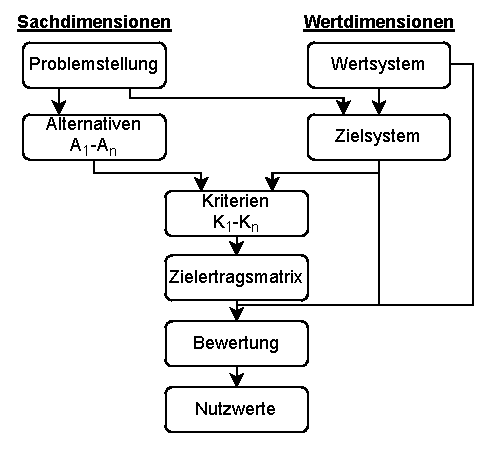
\includegraphics[width=1\textwidth]{img/NutzwertanalyseVorgehenBechmann}}\\ % Pfad
		\source{\cite[Eigene Darstellung in Anlehnung an][27]{Bechmann1978}} % Quelle
		\label{fig:NutzwertanalyseVorgehenBechmann}
	\end{minipage}
\end{figure}

Neben der Problemstellung und der für eine Nutzwertanalyse erforderlichen Lösungsalternativen fließen ebenfalls Entscheidungsregeln und Vorlieben des Autors als Wertesystem, sowie die Vorstellungen vom Zielsystem mit in die Bewertung ein.\footnote{\cite[vgl.][22\psq]{Bechmann1978}}

\enquote{Die zu bewertenden Alternativen werden bezüglich dieses Zielsystems durch Bewertungskriterien beschrieben.}\footnote{\cite[][26]{Bechmann1978}} Die Kriterien werden untereinander anhand ihrer Bedeutung gewichtet, damit wichtigere Kriterien mit höherem Anteil in den Nutzwert eingehen.

Die Gewichtung der Kriterien erfolgt durch die Paarvergleichsmethode. Jeder Teilnehmer der Nutzwertanalyse vergleicht jedes Kriterium gegeneinander. Es muss beim direkten Vergleich immer eine Entscheidung getroffen werden, welches Kriterium der beiden Verglichenen wichtiger ist. Zwei Kriterien dürfen nicht als gleich wichtig gesehen werden.\footnote{\cite[vgl.][15]{Kühnapfel2021b}}

Jeder Teilnehmer hat anschließend die Hälfte der nach der Gaußschen Summenformel (siehe nachfolgende \cref{eq:kleinerGauss}) errechneten Vergleiche durchgeführt, wobei \textit{N} für die Anzahl der Kriterien steht. Es wird nur die Hälfte durchgeführt, weil sich die andere Hälfte der Vergleiche automatisch bedingt. Denn ist \gls{K1} besser als \gls{K2}, so ist \gls{K2} zwangsläufig schlechter als \gls{K1}.

\begin{align*}
	&\,\, \sum_{k=1}^Nk=\frac{N}{2}(N+1) \numberthis \label{eq:kleinerGauss}\\ % Hack with \qquad
	N &= \textmd{Anzahl Kriterien}\\
\end{align*}

Die Summe aller individuellen Vergleiche wird anschließend in einer Vergleichsmatrix zusammengetragen, wie in der nachfolgenden \cref{fig:Praeferenzmatrix} dargestellt. Für jedes Kriterium kann nun die Gesamtsumme der gewonnenen Vergleiche errechnet werden.

\begin{figure}[hbt!]
	\centering
	\begin{minipage}[t]{0.85\textwidth}	
		\caption{Befüllte Präferenzmatrix mit Ergebnissen dreier Teilnehmer}
		\includegraphics[width=1\textwidth]{img/Präferenzmatrix}\\ % Pfad
		\source{\cite[Eigene Darstellung in Anlehnung an][194]{Schierenbeck2016}} % Quelle
		\label{fig:Praeferenzmatrix}
	\end{minipage}
\end{figure}

Aus der Summe der gewonnen Vergleiche je Kriterium wird anschließend der Rang jedes Kriteriums bestimmt. Das Kriterium, welches die meisten Paarvergleiche gewonnen hat, hat den höchsten Rang 1. Das Kriterium, welches die wenigsten Paarvergleiche gewonnen hat, bekommt den niedrigsten Rang N, welcher der Anzahl der Kriterien entspricht. Aus dem Rang kann der inverse Rang ermittelt werden, wie in der nachfolgenden \cref{eq:InverserRang} dargestellt ist.

\begin{align*}
&\qquad\qquad I_j=N + 1 - R_j \numberthis \label{eq:InverserRang}\\ % Hack with \qquad
I_j &= \textmd{Inverser Rang des j-ten Kriteriums}\\
N &= \textmd{Anzahl Kriterien}\\
R_j &= \textmd{Rang des j-ten Kriteriums}
\end{align*}

Aus dem inversen Rang wird anschließend das relative Gewicht jedes Kriteriums mit der nachfolgenden \cref{eq:RelativesGewicht} 
bestimmt.
\begin{align*}
&\qquad\qquad\qquad g_j=\frac{I_j}{\sum_{i=1}^NI_i} \numberthis \label{eq:RelativesGewicht}\\ % Hack with \qquad
g_j &= \textmd{Relatives Gewicht des j-ten Kriteriums}\\
N &= \textmd{Anzahl Kriterien}\\
I_j &= \textmd{Inverser Rang des j-ten Kriteriums}
\end{align*}

Dadurch erhält jedes Kriterium ein relatives Gewicht, welches in der nachfolgenden Nutzwertanalyse zur Gewichtung der Zielerfüllungsgrade genutzt werden kann. Sind alle Kriterien bekannt und gewichtet, so können die Teilnutzwerte der zu vergleichenden Alternativen bestimmt werden. In der nachfolgenden \cref{fig:RechenschemaNutzwertanalyse} ist die Durchführung einer Nutzwertanalyse dargestellt.

\begin{figure}[hbt!]
	\begin{minipage}[t]{1\textwidth}	
		\caption{Rechenschema einer Nutzwertanalyse}
		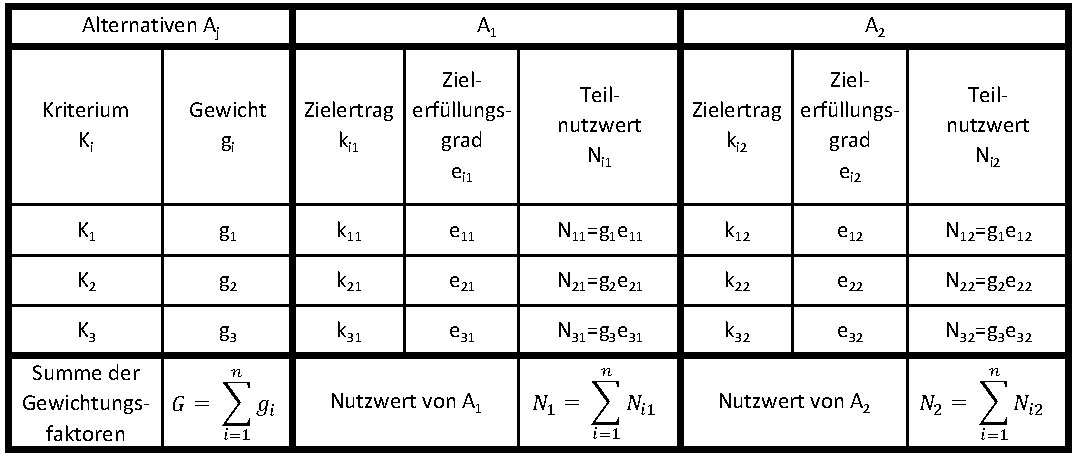
\includegraphics[width=1\textwidth]{img/Rechenschema}\\ % Pfad
		\source{\cite[Eigene Darstellung in Anlehnung an][30]{Bechmann1978}} % Quelle
		\label{fig:RechenschemaNutzwertanalyse}
	\end{minipage}
\end{figure}

Für jede Alternative $A_1$ bis $A_n$ wird der Zielertrag $k_{ij}$ des i-ten Kriteriums der j-ten Alternative bestimmt. Der Zielerfüllungsgrad $e_{ij}$ wandelt den ordinal messbaren Zielertrag jedes i-ten Kriteriums jeder j-ten Alternative in einen kardinal messbaren Wert um.\footnote{\cite[vgl.][29]{Bechmann1978}}  Die Skala der Zielerfüllungsgrade kann nach eigenem Ermessen bestimmt werden und kann beispielsweise von eins bis fünf oder eins bis zehn Punkten reichen.

Wird das Gewicht $g_i$ jedes i-ten Kriteriums mit dem Zielerfüllungsgrad $e_{ij}$ jedes i-ten Kriteriums jeder j-ten Alternative multipliziert, so erhält man den Teilnutzwert $N_{ij}$ jedes i-ten Kriteriums jeder j-ten Alternative. Die Summe aller Teilnutzwerte einer Alternative j ergibt den Nutzwert $N_j$.\footnote{\cite[vgl.][29]{Bechmann1978}}

Wenn dieses Vorgehen für alle j Alternativen wiederholt wird, so ist die Alternative mit dem höchsten Nutzwert die am besten geeignetste Alternative für die gegebene Ausgangsfragestellung.

\subsection{Kriterien für verschiedene Arten der Einbindung}\label{sec:KriterienArtenEinbindung}

In diesem Abschnitt werden die Kriterien definiert, anhand derer im \cref{sec:AnalyseVerschiedenerIntegrationsansaetze} die Arten der Einbindung von Microfrontends bewertet werden.

Ein Kriterium muss, damit es bewert- und vergleichbar ist, messbar sein. Einige Kriterien sind direkt messbar (kardinal), bspw. durch physikalische Größen. Andere Kriterien sind nicht direkt messbar (ordinal), weswegen bei diesen eine Punktevergabe stattfindet, um die ordinale Messbarkeit kardinal messbar zu machen und eine Vergabe von Zielerträgen zu ermöglichen.

Die Punkte für Kriterien werden auf einer Skala von 1 bis 5 vergeben. Ergebnisse von direkt messbaren Kriterien werden miteinander verglichen, nach Optimierungen untersucht und anschließend ebenfalls in einen Punktwert auf der Skala von 1 bis 5 Punkten umgerechnet. Ein Punkt bedeutet, dass das Kriterium nicht erfüllt wurde. Fünf Punkte bedeuten, dass das Kriterium maximal erfüllt wurde. Drei Punkte stehen für eine teilweise Erfüllung. Zwei Punkte für eine geringe und vier Punkte für eine gute Erfüllung.

Nachfolgend werden die Kriterien \textit{Übertragene Datenmenge}, \textit{Renderingzeit}, \textit{Entwicklungsaufwand}, \textit{Wartbarkeit}, \textit{Nähe am Standard}, \textit{Verschiedene Frameworks}, \textit{Kompatibilität}, \textit{Autonomie}, \textit{Unabhängigkeit der Entwicklerteams}, \textit{Lock-In Effekt} und \textit{Interoperabilität} erläutert. 

Die Kriterien entstammen zwei Expertengesprächen, welche im Rahmen der Nutzwertanalyse durchgeführt wurden. Die Protokolle der Gespräche sind in Anhang \ref{app:Expertengespräche} in den \Cref{Exp1,Exp2} nachzulesen.

\textbf{Übertragene Datenmenge}\\
Wenn Microfrontends eingebunden werden, müssen die zur Anzeige benötigten Dateien vom Server oder \gls{CDN} zum Client geladen werden. Je nachdem, mit welcher Art der Einbindung dies geschieht, variiert die Datenmenge. Eine größere Datenmenge die geladen werden muss, bedeutet eine längere Ladezeit bis zur Darstellung des Inhaltes, was besonders bei langsamen Internetverbindungen der Nutzer zu langen initialen Ladezeiten führen kann.

Die Datenmenge der Übertragung kann in Bytes gemessen werden. Die Menge variiert durch die Technologie der Komprimierung, ob Frameworks und Bibliotheken geteilt oder gecached werden und ob die Zusammensetzung der einzelnen Microfrontends serverseitig oder am Client passiert.

Die übertragene Datenmenge ist messbar, wenn der gleiche Inhalt eines Microfrontends bei mehrere Arten der Einbindung verglichen wird. Abzugrenzen ist die Datenmenge, welche der Portalshell zugehörig ist und nicht mit der Art der Einbindung in Verbindung gebracht wird. Die Datenmenge ist besonders relevant, wenn mehrere gleiche Microfrontends nebeneinander eingebunden werden. Im besten Fall skaliert die Datenmenge nicht linear mit den eingebundenen Microfrontends mit, sondern bleibt gleich.

\textbf{Renderingzeit}\\
Die Renderingzeit beschreibt die Zeit, welche vom Aufrufen durch die Portalshell bis zur Anzeige der Microfrontends vergeht. Sie hängt unter anderem mit der übertragenen Datenmenge zusammen, ist aber ebenfalls von der verwendeten Technologie abhängig. Die im Hintergrund ablaufenden Prozesse der Einbindungsarten benötigen unterschiedlich viel Zeit bis zur Darstellung des Inhaltes. Es wird in den nachfolgenden Beispielen in \textit{Time to Usability} gemessen, also bis der gesamte Inhalt geladen und dargestellt wurde. Andere Messverfahren, wie \textit{\gls{TTFB}} oder \textit{\gls{TTFD}}, wurden im Rahmen der Thesis nicht betrachtet.

Damit eine Vergleichbarkeit gegeben ist, muss auch bei diesem Kriterium der Vergleich anhand des selben Inhalts in verschiedenen Arten der Einbindung getätigt werden. Die Messung der Renderingzeit findet in Millisekunden statt.

\textbf{Entwicklungsaufwand}\\
Der Entwicklungsaufwand beschreibt den nötigen Anpassungsbedarf an der Portalshell und den jeweiligen Microfrontends. Im besten Fall bedarf es keiner Anpassung auf beiden Seiten. Es fällt lediglich der Aufwand der einmaligen Einbindung des Microfrontends an. Weitere Einbindungen der gleichen Art verursachen keinen weiteren Aufwand.

Die Summe der Anpassungsaufwände, die an der Portalshell und den Microfrontends entstehen sowie die Aufwände für das einmalige Einbinden und mehrfache Einbinden werden addiert. Die Aufwände werden in Personentagen geschätzt und sind dadurch kardinal messbar.

\textbf{Wartbarkeit}\\
Die Wartbarkeit beschreibt den Aufwand, welcher erbracht werden muss, damit die Art der Einbindung auf Dauer weiterhin funktioniert. Aspekte, wie Häufigkeit von Updates oder nötige Konfigurationsänderungen, werden in der Bewertung berücksichtigt. Besonders bei hohem Entwicklungsaufwand ist Wartbarkeit wichtig. Ein langfristig geringerer Wartungsaufwand rechtfertigt einen initial höheren Entwicklungsaufwand. Die Wartbarkeit ist nicht direkt messbar, kann aber durch gesammelte Aspekte in Punkte umgerechnet werden.

\textbf{Nähe am Standard}\\
Wenn eine Lösung zur Einbindung eines Microfrontends nah am Standard der verwendeten Technologie ist, sind dadurch Risiken, wie bspw. Breaking Changes oder Empfehlung zu einer anderen Lösung unwahrscheinlich. Da die Portalapplikation auf Angular beruht, sollten die Arten der Einbindung Unterstützung durch und zugesicherte Kompatibilität mit dem Angular Framework haben. Wenn das Angular Entwicklerteam Empfehlungen aussprechen würde, eine Art der Einbindung bewusst nicht einzusetzen, würde dies zu Anpassungsaufwänden führen, weil die betroffenen Microfrontends umgebaut werden müssten.

Die Nähe zum Standard ist nicht direkt messbar, kann aber durch Vergleiche der jeweiligen Microfrontend Technologien untereinander und anhand bestehender Statements der Technologiehersteller der Portalshell verglichen werden. 

\textbf{Verschiedene Frameworks}\\
Die Unterstützung verschiedener Web Frameworks bedeutet mehr Flexibilität und Autonomie der Entwicklerteams. Die Angular Portalshell aus dem vorherigen Kapitel wird nicht auf ein anderes Framework migriert.\newline
Die Microfrontends verwenden jeweils nur ein Web Framework, diese können sich aber untereinander unterscheiden. Die Entwicklerteams müssen sich im besten Fall gar nicht gegenseitig abstimmen. Eine direkte Messung ist nicht möglich, allerdings kann eine Tendenz ermittelt werden und Abstufungen möglicher Technologien in verschiedenen Konstellationen festgehalten werden.

\textbf{Kompatibilität}\\
Die Kompatibilität beschreibt, wie gut sich die Art der Einbindung mit anderen Standards und Techniken kombinieren lässt. Eventuell müssen durch die Auswahl einer bestimmten Art der Einbindung einige Features der Portalshell oder der Microfrontends aus- oder umgebaut werden. Eine Liste an sich ausschließenden Verwendungen kann zur Bewertung herangezogen werden. Beispiele hierfür können Designframeworks sein, die miteinander nicht kompatibel sind oder es sind Features wie dynamisches Einbinden oder asynchrones Laden. 

\textbf{Autonomie}\\
Die Autonomie beschreibt, inwieweit das Microfrontend und die Portalshell unabhängig voneinander existieren können. Im besten Fall sind sowohl Microfrontend, als auch die Portalshell, unabhängig voneinander. Im schlechtesten Fall kann das Microfrontend nicht ohne Parameter oder geteilte Bereiche der Portalshell funktionieren. Zur Robustheit sollten die Microfrontends autonom funktionieren.

Auch die Autonomie ist nicht direkt messbar, kann aber ebenfalls durch begründete Aspekte in Punkte umgerechnet werden.

\textbf{Unabhängigkeit der Entwicklerteams}\\
Die Unabhängigkeit der Entwicklerteams beschreibt, wie sehr die Teams, welche an verschiedenen Microfrontends arbeiten, voneinander losgelöst agieren können. Im besten Fall kann jedes Team seine eigenen Entscheidungen treffen und es treten keine Seiteneffekte auf.\newline
Im schlechtesten Fall müssen jegliche Änderungen mit den anderen Entwicklerteams abgesprochen werden und eine autonome Arbeitsweise sowie individuelle Entscheidungsfindungen sind nicht möglich. So müssen sich eventuell Teams untereinander abstimmen, wie sie die gegenseitige Beeinflussung durch Styles und Performance unterbinden.

Dieses Kriterium ist nicht direkt messbar und muss ebenfalls in Punkte umgerechnet werden.

\textbf{Lock-In Effekt}\\
Der Lock-In Effekt beschreibt, wie stark man sich durch Verwendung dieser Art der Einbindung festsetzt. Wenn der initiale Aufwand zum Einrichten der Einbindungsart sehr hoch ist und anschließend der Aufwand zum Wechseln auf eine andere Art ebenfalls sehr hoch ist, besteht ein Lock-In Effekt. Der Lock-In Effekt ist nicht gegeben, wenn durch geringen Aufwand die Art der Einbindung gewechselt werden kann.

Es wird sowohl der Aufwand an der Portalshell, als auch der Aufwand an den Microfrontends bewertet. Ein Lock-In Effekt ist nicht klar definiert und kann daher in Abstufungen vorliegen, welche nicht kardinal messbar sind.

\textbf{Interoperabilität}\\
Die Interoperabilität beschreibt, wie gut Microfrontends durch die Art der Einbindung mit der Portalshell, aber auch anderen Microfrontends interagieren, und kommunizieren können. Zur Interoperabilität zählt das generelle Einbinden und Betreiben dieser Art. Dazu kommen Aspekte, welche sich auf Parameter- und Datenaustausch beziehen.

Bewertet werden können der Aufwand, welcher zum Einrichten von Datenübertragung nötig ist, welche Datentypen übertragen werden können, sowie die Flexibilität, welche die Schnittstellen aufbringen. Ebenfalls gibt es potentielle Konzepte der Kommunikation von Microfrontends untereinander.

Hohe Punktzahl erreichen Lösungen, die eine hohe Interoperabilität aufweisen, welche sich durch einfache, sichere und schnelle Kommunikation mit der Portalshell sowie anderen Microfrontends äußert.

\textbf{Zusammenfassung}\\
In der nachfolgenden \cref{tab:UebersichtKriterien} sind alle elf Kriterien noch einmal aufgelistet. Die Kriterien sind entweder objektiv messbar anhand von Einheiten oder subjektiver Natur, welche aber durch Begründungen und Nachweise belegt werden können.

\begin{table}[hbt]
	\centering
	\begin{minipage}[t]{1\textwidth}	
		\caption{Vergleichskriterien für Arten der Einbindung von Microfrontends}
		\begin{tabularx}{\columnwidth}{|cXX|}
			\toprule
			\textbf{Nr} & \textbf{Kriterium}	& \textbf{Messbar durch} \\
			\midrule
			1 & Übertragene Datenmenge & Differenz Bytes \\
			2 & Renderingzeit & Millisekunden \\
			3 & Entwicklungsaufwand & Personentage \\
			4 & Wartbarkeit & Subjektiv \\
			5 & Nähe am Standard & Subjektiv \\
			6 & Verschiedene Frameworks & Subjektiv \\
			7 & Kompatibilität & Subjektiv \\
			8 & Autonomie & Subjektiv \\
			9 & Unabhängigkeit der Entwicklerteams & Subjektiv \\
			10 & Lock-In Effekt & Subjektiv \\
			11 & Interoperabilität & Subjektiv \\
			\bottomrule
		\end{tabularx}
		\source{Eigene Darstellung}
		\label{tab:UebersichtKriterien}
	\end{minipage}
\end{table}

Die elf Kriterien der vorherigen Tabelle werden im nachfolgenden \cref{sec:GewichtenKriterien} gegeneinander nach Wichtigkeit sortiert und mit einem entsprechendem Gewicht versehen.

\subsection{Gewichtung der Kriterien}\label{sec:GewichtenKriterien}

In diesem Abschnitt wird die Gewichtung der Kriterien, welche im vorherigen \cref{sec:KriterienArtenEinbindung} aufgelistet wurden, nach dem Prozess der in \cref{sec:TheoretischeGrundlagenEinerEvaluierung} erklärten Paarvergleichsmethode vorgenommen.

Das Befüllen der Paarvergleichsmatrix wurde im Rahmen eines Expertengespräches mit fünf Teilnehmern durchgeführt. Die Teilnehmer haben seit mehreren Jahren Erfahrung im Umgang mit Portalapplikationen und setzen sich zusammen aus zwei Software-Architekten, zwei Software-Entwicklern und einem IT-Projektmanager.

Im Prozess des Befüllens der Präferenzmatrix haben alle Teilnehmer individuell jedes Kriterium miteinander vergleichen und dem wichtigeren Kriterium jeweils einen Punkt gegeben.

In der nachfolgenden \cref{fig:Paarvergleichsmethode} ist die ausgefüllte Paarvergleichsmatrix dargestellt, welche die Summe der fünf Einzelbewertungen enthält.

\begin{figure}[hbt!]
	\begin{minipage}[t]{1\textwidth}	
		\caption{Ausgefüllte Paarvergleichsmatrix}
		\includegraphics[width=1\textwidth]{img/AusgefüllteMatrix}\\ % Pfad
		\source{Eigene Darstellung} % Quelle
		\label{fig:Paarvergleichsmethode}
	\end{minipage}
\end{figure}

In der Tabelle ist zu sehen, dass das Kriterium \textit{Interoperabilität} in Summe 39 Punkte erhalten hat und damit knapp vor \textit{Wartbarkeit} mit 38 Punkten und \textit{Unabhängige Entwicklerteams} mit 35 Punkten liegt. 
Die Spalte Rang stellt die Rangfolge der Kriterien absteigend nach ihrer bewerteten Wichtigkeit dar. Anhand des Ranges konnte mit der \cref{eq:InverserRang} der inverse Rang I gebildet werden. Aus dem inversen Rang wurde für jedes Kriterium durch die \cref{eq:RelativesGewicht} das relative Gewicht G bestimmt.

Das wichtigste Kriterium \textit{Interoperabilität} hat somit ein relatives Gewicht von 16,67\% und das von den elf Kriterien am wenigsten wichtig bewertete Kriterium \textit{Datenmenge} wird nur mit 1,52\% gewichtet.

Mit den ermittelten Kriteriengewichten kann nun im nachfolgenden Schritt der Teilnutzwert jedes Kriteriums von jeder Art der Einbindung bestimmt werden.

\subsection{Analyse verschiedener Integrationsansätze}\label{sec:AnalyseVerschiedenerIntegrationsansaetze}

In diesem Abschnitt werden die zur Auswahl stehenden alternativen Arten der Einbindung von Microfrontends in eine Portalshell verglichen. Im nachfolgenden \cref{sec:Abgrenzung Ansaetze} werden dafür zunächst die nicht in Betracht gezogenen Alternativen begründet und abgegrenzt. 
In den darauffolgenden Abschnitten werden anschließend die zum Vergleich ausgewählten Alternativen im Detail für jedes Kriterium untersucht und die jeweilige Erfüllung festgehalten.

\subsubsection{Abgrenzung unpassender Ansätze}\label{sec:Abgrenzung Ansaetze}

Zu Beginn dieser Arbeit wurden in \cref{sec:Portalapplikationen}, \cref{sec:PortalapplikationenHyperlinks} und \cref{sec:Microfrontends} verschiedene Arten der Realisierung von Microfrontends und Portalapplikationen beschrieben.

Portalapplikationen bestehend aus Hyperlinks sind eine einfache Möglichkeit, eine Microfrontend-Architektur darzustellen. Zur Realisierung benötigt es lediglich eine einfache Webseite, welche zu jedem referenzierten Microfrontend einen Link enthält. Bezogen auf die Beispielapplikation aus dem vorherigen \cref{sec:PrototypischesBeispiel} können die Anforderungen in Bezug auf einheitliches Design und eingebundene, kaum spürbare Navigation nicht erfüllt werden. Durch das Klicken auf den Hyperlink wird entweder die gesamte Webseite gewechselt oder die angeklickte Seite öffnet sich in einem neuen Tab.\footnote{\cite[vgl.][]{Steyer2018}} Dieses Verhalten steht der Anforderung von softem Routing diametral entgegen. 

Ebenfalls ist das Übertragen von Parametern von der Portalapplikation zu den Microfrontends erschwert sowie eine Zugriffsbeschränkung auf Teilbereiche ebenfalls nur durch hohen Mehraufwand realisierbar.

Microfrontends durch serverseitiges Rendering sind ebenfalls keine passende Lösung, weil im prototypischem Beispiel eine Angular Portalapplikation gewählt wurde. Angular ist ein Frontend Framework für \gls{SPA}s zum clientseitigen Rendern, welches softes Routing ermöglicht.

In den nachfolgenden vier Abschnitten werden die vier grundlegend zutreffenden Ansätze \textit{Iframe}, \textit{Web Components}, \textit{Module Federation} und \textit{Module Federation mit Web Components} auf die Erfüllung der in \cref{sec:KriterienArtenEinbindung} definierten Kriterien untersucht.

Damit die Kriterienerfüllung vergleichbar ist, wurde für die vier Arten der Einbindung jeweils ein identisches Microfrontend erstellt und in eine prototypische Portalshell eingebunden.

Dieses vergleichbare Microfrontend ist exemplarisch für das Iframe in Anhang \ref{app:Bilder} in \cref{fig:EvalAnsicht} dargestellt. Für die anderen drei Arten der Einbindung wurde ein gleiches Microfrontend erstellt. Lediglich der Name der Einbindungsart in der Überschrift wurde entsprechend ausgetauscht. Die sich dadurch minimal unterscheidende Datenmenge durch mehr oder weniger übertragene Bytes ist zu vernachlässigen.

Das vergleichbare Microfrontend besteht aus einer Überschrift gestyled mit \gls{CSS}, einem Beispielbild sowie einer Angular Material Komponente, konkret einem animierten Fortschrittsbalken.

\subsubsection{Iframe}\label{sec:EvaluierungIFrame}

In diesem Abschnitt wird das Iframe als Microfrontend zur Einbindung in eine Portalshell bewertet. Für die Bewertung werden die im vorherigen \cref{sec:GewichtenKriterien} gewichteten Kriterien verwendet. Die nachfolgenden elf Kriterien sind absteigend nach ermittelten zugehörigen Gewichten sortiert.

Bei den nachfolgend kardinal messbaren Kriterien \textit{Entwicklungsaufwand} , \textit{Renderingzeit} und \textit{Übertragene Datenmenge} werden in diesem Abschnitt bereits die Messergebnisse der anderen drei Einbindungsarten vorweggenommen. Dadurch steht der ermittelte Zielerfüllungsgrad der Alternativen in direktem Vergleich zueinander. Die Begründung oder die Nachweise zum jeweiligen Zielertrag sind in den Abschnitten der Einbindungsarten zu finden.

\textbf{Interoperabilität}\\
Interoperabilität ist der größte Nachteil von Iframes. Der Datenaustausch zur Portalshell und zwischen den Microfrontends ist komplex.

Das Einbinden in die Portalshell ist einfach, solange keine Parameter übertragen werden müssen. Einfache Parameter können über den Querystring von der Portalshell in das Iframe Microfrontend übergeben werden. Dies funktioniert allerdings nur bei nicht sicherheitskritischen Parametern, wie bspw. dem Standort-Parameter einer Wetter-App, denn Parameter über einen Querystring zu übertragen ist nicht sicher und kann manipuliert werden.\footnote{\cite[vgl.][35]{Mezzalira2021}}

Wenn allerdings sicherheitskritische Parameter, die entweder persönliche Informationen enthalten oder nicht modifiziert werden dürfen, vorliegen, dann ist der Querystring nicht geeignet. Dies ist dadurch bedingt, dass der Querystring unter anderem von Administratoren geloggt, aber auch vom Anwender manipuliert werden kann.

Im Fall von informationskritischen Parametern oder benötigter Authentifizierung muss eine sicherere Möglichkeit gefunden werden, um die Parameter zu überreichen und den Anwender zu authentifizieren. Dies kann über gängige Authentifizierungsprotokolle, wie \gls{OIDC} oder \gls{SAML} abgebildet werden.

Im Fall von \gls{SAML} müsste eine Schnittstelle der Portalshell die zu übertragenden Informationen in einem \gls{SAML}-Token verschlüsseln und dann an eine am Microfrontend konfigurierte \gls{SAML}-Schnittstelle als POST-Request übertragen. Die Einbindung einer \gls{SAML}-Schnittstelle kann über eine vom Portalteam bereitgestellte Bibliothek geschehen, was sich aber wiederum negativ auf den initialen Entwicklungsaufwand sowie die Autonomie der Entwicklerteams auswirkt.

Wenn ein Benutzer mehrfach den gleichen Inhalt eines Iframe Microfrontends einbinden möchte, so muss er dies auch mehrfach tun. Iframes skalieren nicht in der Einbindung und teilen auch keine Bibliotheken untereinander oder mit der Portalshell. So kommt es auch zu mehrfachen Requests und die übertragene Datenmenge steigt ebenfalls mit der Anzahl der eingebundenen gleichen IFrames.

Aus diesen Gründen wird das Kriterium \textit{Interoperabilität} mit einer Gewichtung von 16,67\% mit 1 von 5 Punkten bewertet und erhält daher einen Teilnutzwert von 0,1667.

\textbf{Wartbarkeit}\\
Der Aufwand für Wartung bei einem Iframe ist überschaubar. Im Falle einer neuen Version des Microfrontends muss dieses neu veröffentlicht werden, was allerdings durch eine einmalig eingerichtete \gls{CI/CD} Pipeline automatisiert geschehen kann. 

Iframes sind unabhängig von den benutzten Frontend-Frameworks und -Technologien. Von daher sind keine regelmäßigen Updates zu erwarten, auch nicht, wenn sich die Frameworkversion beispielsweise durch ein Update von Angular 12 auf 13 erhöht. Lediglich bei einem Update der \gls{HTML}-Version könnten sich theoretisch Eigenschaften des Iframe-Tags verändern, was aber eher unwahrscheinlich ist.

Das Iframe referenziert ein gehostetes Microfrontend. Wenn eine neue Version des Microfrontends gleichzeitig zu einer Bestandsversion existieren soll, müssten zwei unterschiedliche Versionen des gleichen Microfrontends auf unterschiedlichen URLs gehostet werden. Dies kann beispielsweise bei einem Rollout der Fall sein, bei dem nur konfigurierte Betatester die neuste Version erhalten und Nicht-Betatester die Bestandsversion weiterhin verwenden. 

Dies kann beispielsweise über verschiedene URL-Routen der gleichen Domain realisiert werden. Das Portal muss in dem Fall wissen, für welche User es auf die jeweilige \gls{URL} weiterleiten muss. Ein ähnlicher Ansatz mit dem gleichen Ziel wäre das sogenannte \textit{Blue-Green Deployment}, bei welchem zwei Versionen des Microfrontends gleichzeitig gehostet werden und diese bei Bedarf die genutzte Route wechseln können.\footnote{Mehr Informationen über Blue-Green Deployment unter \cite[][]{CloudFoundryDocumentation2020}}

Ein weiterer negativer Aspekt ist, dass das ganze Microfrontend im Falle einer neuen Version neu veröffentlicht werden muss, was mit einer Ausfallzeit einhergeht.

Die \textit{Wartbarkeit} mit einer Gewichtung von 15,15\% wird mit 3 von 5 Punkten bewertet und erhält dadurch einen Teilnutzwert von 0,4545.

\textbf{Unabhängige Entwicklerteams}\\
Unabhängige Entwicklerteams können durch Iframes realisiert werden. Das Team, welches das Microfrontend betreut, ist grundsätzlich nicht auf andere Teams angewiesen. Es sei denn, man stimmt sich gegenseitig über Schnittstellen ab oder muss den Austausch von sicheren Parametern und Authentifizierung ermöglichen, wie vorher beim Kriterium \textit{Interoperabilität} beschrieben. In dem Fall müssen die zu übertragenden Parameter abgestimmt werden und eine Bibliothek des Portalteams eingebunden werden, die das Auslesen der Parameter übernimmt und die Authentifizierung durchführt.

Wenn das Microfrontendteam nicht in der gleichen Programmiersprache, wie das Portalteam entwickelt, muss das Portalteam eine Schnittstellendokumentation zur Verfügung stellen, anhand derer die Funktionen nachgebaut und die Parameter ausgelesen werden können.

Das Kriterium \textit{Unabhängige Entwicklerteams} mit einer Gewichtung von 13,64\% wird mit 4 von 5 Punkten bewertet, weil lediglich Abhängigkeit zwischen dem Portalteam und dem Microfrontendteam besteht, wenn Authentifizierung oder sicherer Parameteraustausch durchgeführt werden muss. Der Teilnutzwert des Kriteriums beträgt demnach 0,5456.

\textbf{Kompatibilität}\\
Das Iframe wird vollständig mit allem Seitenmarkup in dem \gls{DOM}-Tree der Portalapplikation eingebunden. Dadurch doppeln sich \gls{HTML} Elemente, wie zum Beispiel der Header. Screenreader und Crawler von Suchmaschinen sind durch diese Seitenstruktur häufig verwirrt und erzielen schlechte Resultate.\footnote{\cite[vgl.][]{GoogleSearchCentral2022}}

Ebenfalls weist das Iframe diverse Sicherheitslücken auf, die ausgenutzt werden können. So sind \textit{Iframe Phishing}, \textit{Clickjacking}, \textit{Cross-Frame Scripting} und \textit{Iframe Injection} Sicherheitsrisiken, welche Hacker auf Webseiten mit Iframes ausnutzen können.\footnote{\cite[vgl.][]{Gunawardhana2021}}

Positiv gilt es zu erwähnen, dass das Iframe als einzige Art der Einbindung für veraltete Browser zugänglich ist und sogar im Internet Explorer seit jeher verwendet werden kann.\footnote{\cite[vgl.][]{MDNWebDocs2021a}}

Das Kriterium \textit{Kompatibilität} mit einer Gewichtung von 12,12\% wird mit einem Punkt bewertet und erhält dadurch einen Teilnutzwert von 0,1212.

\textbf{Autonomie}\\
Da der Iframe-Tag eine gehostete Webseite einbindet, läuft die eingebundene Applikation grundsätzlich autonom. Eine Applikation, welche keine mandantenspezifischen Parameter benötigt läuft dementsprechend komplett selbstständig. Eine Applikation, welche Inputparameter der Portalshell benötigt, wie beispielsweise eine Wetter-App, funktioniert ohne die benötigten Standort-Parameter nicht.

Ein weiterer Vorteil ist, dass das Iframe die Portalshell nicht beeinflussen kann. So sind die Stylings abgekapselt. Das Microfrontend und die Portalshell beeinflussen sich nicht gegenseitig.\footnote{\cite[vgl.][35]{Geers2020}} Dies ist in Anhang \ref{app:Bilder} in \cref{fig:EvalIframeBeeinflussung} dargestellt. Der rot umrandete Bereich ist das Iframe, welches die Background-Color von allen Überschriften rot setzt. Alles außerhalb des roten Rahmens sind Elemente von der Portalshell und dort haben Überschriften eine blaue Hintergrundfarbe. Es findet keine gegenseitige Beeinflussung statt.

Das Kriterium \textit{Autonomie} mit einer Gewichtung von 10,61\% wird mit 5 von 5 Punkten bewertet und erhält dadurch einen Teilnutzwert von 0,5305. Nur verlinkte Portalapplikationen haben eine noch höhere Autonomie.

\textbf{Nähe zum Standard}\\
Das Iframe ist ein offiziell anerkanntes \gls{HTML} Element, welches bereits seit vielen Jahren besteht. Alle Browser unterstützen das Iframe mit den grundlegenden Parametern \texttt{src}, \texttt{height} und \texttt{width}.\footnote{\cite[vgl.][]{MDNWebDocs2021a}} Alle Frontend Frameworks, welche \gls{HTML} einsetzen, können Iframes einbinden.

Das Kriterium \textit{Nähe zum Standard} mit einer Gewichtung von 9,09\% wird mit 5 von 5 Punkten bewertet und erhält dadurch einen Teilnutzwert von 0,4545.

\textbf{Verschiedene Frameworks}\\
Mit einem Iframe gibt es kaum Beschränkungen und Inkompatibilitäten zu anderen Frameworks. Da das Iframe durch einen \gls{HTML}-Tag eingebunden wird, ist es mit allen Frontend-Frameworks kompatibel, welche \gls{HTML} nutzen. Weniger Beschränkungen gäbe es nur noch bei reinen Applikationen auf der Basis von Links.

Das Iframe bietet sich für legacy Anwendungen an, die nicht auf moderne Web-Frameworks umgebaut werden können. Die Art der Einbindung kostet wenig Budget und ist schnell umsetzbar. Auch kann der Iframe Inhalt serverseitig gerendert werden, selbst wenn die Portalshell beispielsweise clientseitig gerendert wird.

Deswegen wird das Kriterium \textit{Frameworks} mit einer Gewichtung von 7,58\% mit 5 von 5 Punkten bewertet und erhält dadurch einen Teilnutzwert von 0,3790.

\textbf{Entwicklungsaufwand}\\
In der nachfolgenden \cref{tab:GGAufwand} wird eine Gegenüberstellung des Entwicklungsaufwandes bei verschiedenen Arten der Einbindung vorgenommen. Alle vier Arten wurden nach initialem Entwicklungsaufwand, Aufwand der bei Änderung an Features entsteht und Aufwand, welcher bei Einbindung des gleichen Microfrontends an einer anderen Stelle der Portalapplikation auftritt, bewertet. Letzteres findet häufig bei Portalapplikationen mit Mandantenkontext Anwendung. Verschiedene Mandanten rufen das gleiche Microfrontend mit unterschiedlichen, mandantenindividuellen Parametern auf.

Die Bewertungsskala reicht von ++ (sehr gut), über + (gut), o (neutral), - (schlecht) bis hin zu - - (sehr schlecht). Ein sehr geringer Aufwand erhält ein ++. Ein sehr hoher Aufwand bekommt eine sehr schlechte (- -) Bewertung. Der Gesamtaufwand wird in \gls{PT} geschätzt. Ein \gls{PT} entspricht 8 Stunden.

\begin{table}[!hbt]
	\centering
	\begin{minipage}[t]{1\textwidth}	
		\caption{Entwicklungsaufwand verschiedener Microfrontends} % Überschrift
		\begin{tabularx}{\columnwidth}{| X || c | c | c | c |}
			\toprule
			\thead{\textbf{Art der}\\ \textbf{Einbindung}} & \thead{\textbf{Initialer}\\ \textbf{Aufwand}} &
			\thead{\textbf{Anpassungs-} \\\textbf{aufwand}} & \thead{\textbf{Aufwand}\\ \textbf{mehrfache}\\ \textbf{Einbindung}} & \thead{\textbf{Geschätzter}\\ \textbf{Aufwand PT}}\\
			\midrule
			Iframe & ++ & - & o & 0,75\\
			Web Component & + & - & ++ & 1\\
			Module Federation & - & + & + & 2 \\
			Module Federation WC & - - & - & + & 2,5\\
			\bottomrule
		\end{tabularx}
		\source{Eigene Darstellung}
		\label{tab:GGAufwand}
	\end{minipage}
\end{table}

Der initiale Entwicklungsaufwand ist bei einer Einbindung über ein Iframe gering. So muss das Microfrontend lediglich entwickelt werden und auf einer Webseite veröffentlicht sein, die das Einbinden über den \textit{\gls{CORSHeader}} erlaubt.

Bei der einbindenden Portalapplikation muss der Iframe \gls{HTML}-Tag konfiguriert werden. Der src-Parameter zeigt auf die \gls{URL} des veröffentlichten Microfrontends. Es empfiehlt sich, das standardmäßige Styling zu überschreiben, damit die Höhe und Breite dem angezeigten Content entsprechen und der standardmäßige Rand entfernt wird. Ebenfalls sollte die Einbindung so gebaut werden, dass sie dynamisch geschieht und nicht direkt im Code referenziert wird.

Der Aufwand dafür ist gering, sodass das Iframe bereits nach wenigen Minuten angezeigt werden kann. Noch schneller ginge nur das direkte Einbinden eines Links, wie es in \cref{sec:PortalapplikationenHyperlinks} beschrieben wurde. Die Einbindung des Iframes skaliert nicht, das heißt es muss jedes mal wieder ein iframe-Tag eingebunden werden. Ändern sich die Hosting-URL oder die benötigten Parameter der Iframe-Webseite, so funktioniert die Einbindung nicht mehr und muss angepasst werden.

Aus diesem Grund wird das Kriterium \textit{Entwicklungsaufwand} bei einem Iframe mit 4 von 5 Punkten bewertet. Bei der Gewichtung des Kriteriums von 6,06\% wird ein Teilnutzwert von 0,2424 erreicht.

\textbf{Renderingzeit}\\
Die Renderingzeit für Iframes ist, wie in der nachfolgenden \cref{tab:MessungenEvaluierung} dargestellt, mit 480ms die höchste von allen vier verglichenen Arten der Einbindung. Eine halbe Sekunde ist eine spürbare Verzögerung beim Aufrufen einer Seite. Allerdings stellt eine halbe Sekunde dennoch eine ertragbare Wartezeit beim Arbeiten mit der Webseite dar.\footnote{\cite[vgl.][]{unbounce2022}}

\begin{table}[!hbt]
	\centering
	\begin{minipage}[t]{1\textwidth}	
		\caption{Übersicht Datenmenge \& Renderingzeit von Einbindungsarten} % Überschrift
		\begin{tabularx}{\columnwidth}{| X | c | c | c |}
			\toprule
			\thead{\textbf{Art der}\\ \textbf{Einbindung}} & \thead{\textbf{Datenmenge in KB}} &
			\thead{\textbf{Datenmenge mit}\\ \textbf{großer Bibliothek}} & \thead{\textbf{Renderingzeit}\\ \textbf{in ms}}\\
			\midrule
			Iframe & 1949 & 2254  & 480 \\
			Web Component & 1824 & 2205 & 60 \\
			Module Federation & 2523 & 2524 & 39 \\
			Module Federation WC & 2609 & 2611 & 23 \\
			\bottomrule
		\end{tabularx}
		\source{Eigene Darstellung}
		\label{tab:MessungenEvaluierung}
	\end{minipage}
\end{table}

Die Daten aus der Tabelle entstammen Messungen, welche in Anhang \ref{app:Bilder} in den \crefrange{fig:MessungIFrame}{fig:MessungMFWC} dargestellt sind. Die Messungen wurden mit dem gleichen Microfrontend durchgeführt, welches durch unterschiedliche Arten eingebunden wurde. Damit die Messungen nachvollzogen werden können, ist in Anhang \ref{app:Bilder} in \cref{fig:Laborsetup} das Laborsetup mit den Messbedingungen dargestellt.

Dadurch, dass die anderen drei Arten Renderingzeiten im zweistelligen Millisekunden haben, wird das Iframe nur mit 2 von 5 Punkten bewertet. Durch die Gewichtung des Kriteriums \textit{Renderingzeit} von 4,55\% erreicht das Iframe einen Teilnutzwert von 0,0910.

\textbf{Lock-In Effekt}\\
Bei einer Einbindung durch ein Iframe entsteht kein Lock-In Effekt. Es wird weder auf Seiten des Microfrontends, noch auf Seiten der Portalshell eine proprietäre Technologie eingesetzt. Auf Seiten des Microfrontends bedarf es keiner Anpassung. Bei der Portalshell muss zum Entfernen des Iframes lediglich der einbindende HTML-Tag gelöscht werden.

Jede der drei nachfolgenden Arten der Einbindung kann autonom funktionieren und dadurch als Iframe eingebunden werden. Beispielsweise kann die Web Component sich selbst in der Index.html einbinden, wie exemplarisch in \cref{list:SelbstEinbindenWC} in Anhang \ref{app:Listing} zu sehen ist. Anschließend kann die Index.html als Iframe in einer Portalapplikation eingebunden werden.

Selbiges gilt für die Einbindungen über Module Federation. Das Modul, welches standardmäßig exportiert wird, kann auch von einem Iframe eingebunden werden.

Das Kriterium \textit{Lock-In Effekt} mit einer Gewichtung von 3,03\% wird mit 5 von 5 Punkten bewertet und erhält dadurch einen Teilnutzwert von 0,1515.

\textbf{Übertragene Datenmenge}\\
In der vorherigen \cref{tab:MessungenEvaluierung} wurde bei den vier Arten der Einbindung jeweils die übertragene Datenmenge sowie die benötigte Renderingzeit gemessen und gegenübergestellt. Das Iframe weist mit 1949 \gls{KB} im normalen Anwendungsfall und 2254 \gls{KB} bei Verwendung einer großen Bibliothek verglichen mit den anderen Arten geringe Werte auf. So überträgt das Iframe, knapp hinter der Web Component, die geringste Datenmenge zum Client.

Dennoch ist die Datenmenge bei einem Iframe nicht skalierbar. Werden mehrere Bibliotheken im Iframe eingebunden, so werden diese alle zum Client übertragen. Werden mehrere Iframes auf einer Seite eingebunden, so werden alle Bibliotheken aller Iframes übertragen. Die übertragene Datenmenge skaliert linear mit der Anzahl der eingebundenen Iframes. Dies ist exemplarisch in der \cref{fig:EvalIframeSkalierbarkeit} in Anhang \ref{app:Bilder} mit zwei Iframes auf der gleichen Seite dargestellt. Für beide werden der Code sowie die Bibliotheken zum Client geladen.

Die übertragende Datenmenge setzt sich aus der generierten \gls{JS}-Datei, welche die Bibliotheken beinhalten, sowie den Stylings zusammen. Bibliotheken oder Assets können nicht geteilt werden. Bei dem Iframe wird der gesamte \gls{HTML}-Inhalt der eingebundenen Webseite in das HTML der Portalshell gerendert, wodurch Overhead entsteht (siehe \cref{fig:IFrameHTML} in Anhang \ref{app:Bilder}).

Das Kriterium \textit{Datenmenge} mit einer Gewichtung von 1,52\% wird daher mit nur einem von fünf möglichen Punkten bewertet und erhält dadurch einen Teilnutzwert von 0,0152.

\textbf{Zwischenfazit}\\
Das Iframe ist eine schnelle Lösung, welches sich für veraltete Anwendungen anbietet, in die nicht mehr investiert werden soll. Allerdings ist die Interoperabilität nicht ausgeprägt und besonders komplexe Einbindungen mit vielen geteilten Parametern, Sicherheitsanforderungen und bidirektionalem Austausch sind nicht geeignet. Ebenfalls sind Ladezeiten sowie Datenmenge nicht optimiert und skalieren nicht.

\subsubsection{Web Components}\label{sec:EvaluierungWebComponents}

In diesem Abschnitt wird die Web Component als Art der Einbindung in eine Portalshell untersucht. Die Web Component wird, wie das Iframe im vorherigen \cref{sec:EvaluierungIFrame}, auf die Erfüllung der elf gewichteten Kriterien aus \cref{sec:GewichtenKriterien} geprüft.

\textbf{Interoperabilität}\\
In Microfrontends durch Web Components können mittels Parametern Daten von der Portalshell entgegengenommen werden. Durch diese Parameter kann das Microfrontend individuell auf die Bedürfnisse des aktuellen Benutzers, dessen Mandanten und der Portalshell angepasst werden. Im Beispiel eines Wetter-Microfrontends könnten die Standort-Daten des Nutzers übertragen werden, sodass diesem immer das aktuelle Wetter angezeigt wird.

Muss der Nutzer im Microfrontend authentifiziert werden, ist der Prozess aufwändiger. Die Portalshell muss der Web Component einen \gls{OIDC} Token übergeben, welcher vom Microfrontend genutzt wird, um einen Aufruf an das Backend der Portalshell zu tätigen. Die Portalshell verifiziert die Aufrufe des Microfrontends und gibt Daten für autorisierte Endpunkte zurück.

Die Web Component kann über Komponentenbibliotheken mit anderen Microfrontends oder der Portalshell kommunizieren und Daten austauschen. Alternativ kann die Kommunikation zwischen den Microfrontends und der Portalshell auch über Events geschehen, auf die die Empfänger reagieren. So kann beispielsweise bei einer Web Component Tabelle mit \textit{infinite scroll}-Feature ein Event gesendet werden, sobald der Benutzer am unteren Tabellenrand angekommen ist und die Portalshell weitere Einträge liefern soll.\footnote{\cite[vgl.][]{Rauber2020d}}

Im Gegensatz zum Iframe reicht die einmalige Einbindung einer Web Component und anschließend kann das Microfrontend mehrfach aufgerufen und eingebunden werden.

Das Kriterium \textit{Interoperabilität} mit einer Gewichtung von 16,67\% wird mit 4 von 5 Punkten bewertet und erhält dadurch einen Teilnutzwert von 0,6668.

\textbf{Wartbarkeit}\\
Der Wartungsaufwand für Web Components ist ebenfalls gering. Wenn eine Web Component einmal gebaut wurde, kann sie in alle anderen Applikationen eingebunden werden. Es existieren Onlineplattformen, welche veröffentliche Web Components verwalten und Einbindung dieser in andere Applikationen ermöglichen, wie bspw. \url{https://www.webcomponents.org/}.

Die Verwaltung von internen Web Components muss aber nicht zwingend über einen Paketmanager geschehen, sondern kann auch über einen erreichbaren Speicherort gelöst werden (bspw. einen Azure Storage Account). Im Storage liegt dann in einem Unterordner, welcher nach der Version benannt ist, die kompilierte \gls{JS}-Datei. Die Portalshell kann dann nach Mitteilung des Web Component Teams eine neue Version manuell einbinden, wofür der Direktlink zur Datei ausreicht.

Das Ablegen der Dateien im Storage oder Paketmanager kann durch eine \gls{CI/CD} Pipeline automatisiert werden. Auch das Abrufen sowie Einbinden der Versionen in der Portalshell kann automatisiert geschehen. Es ist zeitgleich möglich, mehrere verschiedene Versionen der gleichen Web Component einzubinden, solange der \gls{HTML}-Tag sich für jede Version unterscheidet.

Das Kriterium \textit{Wartbarkeit} mit einer Gewichtung von 15,15\% wird mit 4 von 5 Punkten bewertet und erhält dadurch einen Teilnutzwert von 0,6060.

\textbf{Unabhängige Entwicklerteams}\\
Das Microfrontend Team kann bei Web Components unabhängig vom Entwicklungsteam der Portalshell agieren. Denn das Team, welches die Web Component betreut kann jederzeit eine neue Version der Web Component veröffentlichen, solange sie die alte Version nicht überschreiben.

Über Paketmanager, wie den \gls{NPM} oder Yarn, können Web Components in verschiedenen Version veröffentlicht werden. So bleibt eine Historie der Web Components erhalten und das Portalshellteam kann je nach Bedarf die neueste oder eine ältere Version einbinden. 

Vorteile eines Paketmanagers sind, dass öffentliche Web Components kostenfrei eingebunden werden können. Der Sourcecode von internen Web Components sollte privat bleiben, was aber nur durch Bezahlmodelle gelöst werden kann (bspw. \gls{NPM} Organizations).\footnote{\cite[vgl.][]{npm2022}} Eine eigens kreierte Lösung ist dahingegen kostenfrei, allerdings nicht vergleichbar flexibel mit Versionen und der automatischen Einbindung.

Aus dem Grund, dass Web Components Kompatibilitätsprobleme mit einigen Design-frameworks haben, sind die Teams in ihrer Entscheidungsauswahl eingeschränkt. Eventuell müssen Bestandslösungen angepasst oder Neuentwicklungen mit anderen Design-Komponenten gebaut werden.

Das Kriterium \textit{Unabhängige Entwicklerteams} mit einer Gewichtung von 13,64\% wird für Web Components daher mit 3 von 5 Punkten bewertet und erhält dadurch einen Teilnutzwert von 0,4092.

\textbf{Kompatibilität}\\
Web Components basieren auf den Grundlagen von \gls{JS} sowie \gls{HTML} und sind daher unabhängig von Frontend-Frameworks einsetzbar.

Sie werden von den modernen Browsern wie Chrome, Edge, Firefox und Opera vollumfänglich unterstützt. Safari unterstützt einige der Web Components Features, aber nicht alle. Der Internet Explorer kann keine Web Components darstellen.\footnote{\cite[vgl.][]{MDNWebDocs2022a}} Der Internet Explorer wird ab Mitte 2022 offiziell nicht mehr von Microsoft unterstützt.\footnote{\cite[vgl.][]{Microsoft2021b}} Er wurde weitestgehend durch den Edge-Browser ersetzt und ist im Jahre 2022 nur noch bei weniger als einem Prozent der deutschen Nutzer im Einsatz.\footnote{Vgl. \cref{fig:StatistikBrowser} in Anhang \ref{app:Bilder}}

Durch die Einbindung von Web Components im Shadow \gls{DOM} wird verhindert, dass Stylings der Komponente die Portalshell beeinflussen. Allerdings entstehen dadurch Probleme mit Design Frameworks, die auf globale Styles setzen. Bei Angular Material\footnote{\cite[vgl.][]{Github2021}} oder Twitter Bootstrap\footnote{\cite[vgl.][96]{Geers2020}} kann es deshalb zu Problemen bei der Darstellung kommen. Dies kann aber durch das Einbinden der Styles in der Komponente oder durch das Entfernen der Shadow DOM Einbindung gelöst werden. Weitere Informationen zu Shadow DOM sind im nachfolgenden Kriterium \textit{Autonomie} beschrieben.

Das Kriterium \textit{Kompatibilität} mit einer Gewichtung von 12,12\% wird daher mit 3 von 5 Punkten bewertet und erhält somit einen Teilnutzwert von 0,3636.

\textbf{Autonomie}\\
Angular Komponenten, welche zu einer Web Component definiert werden, haben verschiedene Ausprägungen der sogenannten \textit{encapsulation policy}, welche die Reichweite des Stylings der Komponente steuert. Die Ausprägung \texttt{ViewEncapsulation.None} bedeutet, dass keine Kapselung des Stylings geschieht und die Stylings auch andere Komponenten betreffen könnten. Bei
\texttt{ViewEncapsulation.Emulated} werden die Dateien der Web Component an einen emulierten, gekapselten DOM-Tree des Browsers angehangen und wirken nur dort beschränkt. Durch \texttt{ViewEncapsulation.ShadowDom} wird die Shadow DOM API des Browsers genutzt und die Stylings dadurch beschränkt.\footnote{\cite[vgl.][]{Angular2022a}}

Die Stylings des Microfrontends können andere Elemente der Portalshell im Modus \texttt{ViewEncapsulation.ShadowDom} nicht beeinflussen. Allerdings können dadurch Probleme mit dem Styling einiger eingebundener Komponenten in der Web Component entstehen, wie beispielsweise die fehlerhafte Darstellung von Angular Material Komponenten.\footnote{\cite[vgl.][]{Handler2020}}

Das Kriterium \textit{Autonomie} mit einer Gewichtung von 10,61\% wird daher mit 4 von 5 Punkten bewertet und erhält dadurch einen Teilnutzwert von 0,4244.

\textbf{Nähe zum Standard}\\
Web Components und die dazugehörigen Features, wie customElements, \gls{HTML} Templates und Shadow DOM, sind Standards der Web Entwicklung.\footnote{\cite[vgl.][]{MDNWebDocs2022a}}

Von daher sind Web Components eine Lösung, welche dem Standard entspricht. Das Kriterium \textit{Nähe zum Standard} mit einer Gewichtung von 9,09\% wird dementsprechend mit 5 von 5 Punkten bewertet und erhält dadurch einen Teilnutzwert von 0,4545.

\textbf{Verschiedene Frameworks}\\
Die Webseite \url{https://custom-elements-everywhere.com/} prüft diverse Frontend Frameworks bei jedem Update automatisiert auf die Kompatibilität zur customElements-API.\footnote{\cite[vgl.][]{CustomElementsEverywhere2022}}

Zum Zeitpunkt der Erstellung werden unter anderem \textit{Vue.js}, \textit{React}, \textit{Angular}, \textit{AngularJS} und \textit{Svelte} mit positivem Testergebnis ausgewiesen. Die relevanten Frameworks zur Erstellung von Web Components sind dadurch kompatibel und decken sich ebenfalls mit vielen der populärsten Web Frameworks (vgl. \cref{fig:WebFrameworks} in Anhang \ref{app:Bilder}).

Das Kriterium \textit{Frameworks} mit einer Gewichtung von 7,58\% wird daher mit 4 von 5 Punkten bewertet und erhält dadurch einen Teilnutzwert von 0,3032.

\textbf{Entwicklungsaufwand}\\
in Anhang \ref{app:Listing} in \cref{lst:MFWCAppModule} und \cref{list:WCInjectionComponent} ist zu sehen, welche Codeanpassungen zum Einbinden einer Web Component auf Seiten der Portalshell und des Microfrontends nötig sind.
Bei dem Microfrontend muss in der \texttt{app.module.ts} die Angular Komponente, welche exportiert werden soll, als \texttt{customElement} definiert werden. Wird das gleiche Element zweifach definiert, kommt es zu Fehlern, weswegen vorher geprüft wird, ob bereits ein Element mit dem Namen besteht. Anschließend kann das Microfrontend gebaut und die \texttt{main.js} in die Portalshell eingebunden werden.

Damit die Portalshell eine Web Component einbinden kann, müssen drei Aspekte bekannt sein. Die \gls{URL} der \texttt{main.js}, der Name des \textit{customElements} und ob Parameter mit übergeben werden sollen. Die Portalshell muss eine Möglichkeit zur Verfügung stellen, welche die Einbindung der Web Component übernimmt (bspw. eine Angular Komponente). 

Die Komponente der Portalshell muss den \gls{JS}-Code laden, ein neues Script-Tag in das HTML-Dokument der Portalshell einfügen und die \gls{URL} der Web Component auf die \texttt{src} Property des Script-Tags setzen, wie in Anhang \ref{app:Listing} unter \cref{list:WCInjectionComponent} zu sehen ist. Anschließend wird der \texttt{createElement}-Methode der Name des definierten HTML-Elements übergeben und dadurch die Web Component eingebunden.

Der Aufwand ist etwas höher als bei einem Iframe, aber in Summe dennoch überschaubar. Wenn die Methoden zum Einbinden entwickelt wurden, können sie gut wiederverwendet werden. Das Microfrontend kann nach einmaliger Konfiguration mehrfach eingebunden werden, bei Bedarf auch mit unterschiedlichen Parametern. In \cref{tab:GGAufwand} wurde deswegen die Web Component mit einer guten Wertung beim initialen Aufwand und einer sehr guten Wertung beim mehrfachen Verwenden versehen. Die schlechte Wertung beim Anpassungsaufwand bedingt sich durch den Anpassungsbedarf, wenn Parameter oder die URL der \gls{JS}-Datei sich ändern.

Das Kriterium \textit{Entwicklungsaufwand} mit einer Gewichtung von 6,06\% wird mit 4 von 5 Punkten bewertet und erhält dadurch einen Teilnutzwert von 0,2424.

\textbf{Renderingzeit}\\
In der im vorherigen Abschnitt aufgestellten \cref{tab:MessungenEvaluierung} weist die Web Component als Art der Einbindung eine Renderingzeit von 60ms auf. Damit ist diese Art zwar nur die Drittschnellste, aber eine Renderingzeit im zweistelligen Millisekundenbereich ist ausreichend schnell und stört den Nutzer nicht merklich.

Dadurch wird das Kriterium \textit{Renderingzeit} mit 3 von 5 Punkten bewertet und erreicht bei einer Gewichtung von 4,55\% einen Teilnutzwert von 0,1365.

\textbf{Lock-In Effekt}\\
Ein Lock-In Effekt liegt bei Web Components nicht vor. Die Web Component ist, wie bereits beim Kriterium \textit{Nähe zum Standard} erläutert, ein anerkannter Standard von \gls{HTML} und \gls{JS}. Sollte man sich in Zukunft gegen Web Components entscheiden, kann das Microfrontend der Web Component auch ohne nennenswerten Mehraufwand direkt als Iframe eingebunden werden.

In Anhang \ref{app:Listing} in \cref{list:SelbstEinbindenWC} ist der nötige Code zu sehen, dessen es bedarf, damit ein Web Component Microfrontend sich selbst einbindet. Es reicht den vorher definierten \gls{HTML}-Tag in die \texttt{index.html} einzufügen. Das Ergebnis der Selbsteinbindung ist in Anhang \ref{app:Bilder} unter \cref{fig:WCSelbstEinbindung} dargestellt.  Nach dieser Einbindung kann die Webseite des Microfrontends veröffentlicht und in andere Applikationen als Iframe eingebunden werden. Es entsteht daher kein Lock-In Effekt.

Deswegen erhält \textit{Lock-In Effekt} 5 von 5 möglichen Punkten, was bei der ermittelten Gewichtung von 3,03\% zu einem Teilnutzwert von 0,1515 führt.

\textbf{Datenmenge}\\
Die Datenmenge eines vergleichbaren Microfrontends hat im einheitlichen Test mit 1824\gls{KB} die geringste Datenmenge der vier verglichenen Arten der Einbindung erreicht (siehe \cref{tab:MessungenEvaluierung}). Wurde eine große Bibliothek in der Web Component verwendet, so werden 2205\gls{KB} zum Client übertragen. Die Skalierung der übertragenen Dateigröße gleicht der beim Iframe.

Ist die gleiche Web Component in mehreren Microfrontends in der Portalshell eingebunden, steigt die Datenmenge nicht linear zur Anzahl der Microfrontends an, wie es beim Iframe der Fall ist. Die Web Component wird clientseitig durch den Browser gecached und muss somit nur einmalig geladen werden.\footnote{Siehe \cref{fig:EvalWCSkalierbarkeit} in Anhang \ref{app:Bilder}}

Im nachfolgenden \cref{sec:EvaluierungModuleFederationWC} wird ein Vergleich der übertragenen Datenmenge bei einem Microfrontend mit mehreren eingebundenen Bibliotheken mit Web Components und Module Federation mit Web Components durchgeführt. Der Vergleich zeigt, dass, ab einer bestimmten Summe der Datenmenge von geteilten Bibliotheken, die Einbindung über Module Federation in einer geringeren zum Client übertragenen Datenmenge resultiert. Wird dieser Punkt jedoch nicht überschritten, so sind Web Components sinnvoller.

Das Kriterium \textit{Datenmenge} mit einer Gewichtung von 1,52\% wird mit 4 von 5 Punkten bewertet und erhält dadurch einen Teilnutzwert von 0,0608.

\textbf{Zwischenfazit}\\
In diesem Abschnitt wurden Web Components als Art der Einbindung in eine Portalshell untersucht. Die Web Components weisen Stärken bei der Skalierbarkeit, der Kompatibilität, der Datenmenge bei kleinen Bibliotheken und bei der Kapselung der Inhalte auf. Allerdings entstehen durch die Kapselung auch Probleme bei der Anzeige und bei großen eingebundenen Bibliotheken ist die übertragene Datenmenge nicht optimal.

\subsubsection{Module Federation mit Angular Modulen}\label{sec:EvaluierungModuleFederation}

In diesem Abschnitt wird Module Federation mit Angular Modulen als Einbindungsart eines Microfrontends in eine Portalshell bewertet. Dies geschieht, wie bei den beiden vorherigen Abschnitten, durch die Feststellung der Erfüllung der in \cref{sec:GewichtenKriterien} gewichteten Kriterien.

\textbf{Interoperabilität}\\
Module Federation teilt Daten von der Portalshell zum Microfrontend nicht über Parameter, wie es bei den beiden vorherigen Arten der Fall war, sondern über \textit{\gls{Lib}s}. Diese beinhalten einen Service und optional weitere Logik.\footnote{\cite[vgl.][63]{Steyer2020}} 

Ein Beispiel dafür ist in Anhang \ref{app:Bilder} unter \cref{fig:ModuleFShareData} dargestellt. Dieses zeigt eine \gls{Lib} zur Authentifizierung, welche Informationen über den angemeldeten User von der Portalshell zum Microfrontend reicht. Der User loggt sich auf der Loginmaske mit seinen Daten ein. Die Portalshell validiert die Logindaten und speichert den Namen des Users anschließend in einem Service der \gls{Lib}, auf welchen das Module Federation Microfrontend zugreifen kann.

Damit Parameter an das Module Federation Microfrontend übergeben werden können, sollte dafür also eine Lib erstellt werden. Die Lib muss vom Portalteam verwaltet sowie unter Umständen erweitert werden können. Sie beinhaltet die Parameter, welche für die Microfrontends notwendig sind. Eine Lib zu erstellen bedeutet mehr Aufwand, als nur Parameter zu übergeben, wie bspw. bei der Web Component. Allerdings können darüber auch komplexe Logiken abgebildet werden, wie beispielsweise eine Auth0-Implementierung zur Authentifizierung.\footnote{\cite[vgl.][]{Steyer2022a}}

Die Microfrontends, welche durch Module Federation in die Portalshell eingebunden sind, werden durch sogenanntes \textit{lazy loading} verzögert eingebunden. Dies ist eine Ausnahme gegenüber anderen Arten der Einbindung, bei denen jeglicher Code zur Compilezeit bekannt sein muss.\footnote{\cite[vgl.][]{Steyer2021c}} Die asynchrone Einbindung wirkt sich jedoch positiv auf die initiale Renderingzeit der Portalshell aus.

Das Kriterium \textit{Interoperabilität} mit einer Gewichtung von 16,67\% wird daher mit 5 von 5 Punkten bewertet und erhält somit einen Teilnutzwert von 0,8335.

\textbf{Wartbarkeit}\\
In Zukunft sind Updates für Module Federation zu erwarten, weil die Art der Einbindung erst seit Anfang 2020 und damit seit aktuell ca. zwei Jahren zur Verfügung steht.\footnote{\cite[vgl.][]{Jackson2020b}} Durch produktiven Einsatz in Unternehmenskontexten können sich in Zukunft noch neue Anforderungen ergeben. Updates der Webpack Version oder der Module Federation Hilfsbibliotheken sind in Zukunft zu erwarten und müssen bei allen Microfrontends sowie der Portalshell zeitgleich eingespielt werden.

In der offiziellen Webpack Dokumentation zu Module Federation sind zwei beispielhafte Anwendungsszenarien skizziert. So kann eine von mehreren anderen Microfrontends genutzte Bibliothek veröffentlicht und über Module Federation eingebunden werden. Dies können sich verteilte Teams zu Nutzen machen. Für die geteilte Bibliothek kann bei Bedarf einzeln ein Update eingespielt werden, ohne dass alle abhängigen Microfrontends ebenfalls neu veröffentlicht werden müssen.\footnote{\cite[vgl.][]{Webpack2020b}} Dies stärkt die Wartbarkeit sowie die Autonomie der zugehörigen Microfrontends.

Dadurch erhält das Kriterium \textit{Wartbarkeit} 4 von 5 möglichen Punkten, was bei der Gewichtung von 15,15\% zu einem Teilnutzwert von 0,6060 führt.

\textbf{Unabhängige Entwicklerteams}\\
Das Entwicklerteam des Microfrontends kann unabhängig von Entwicklerteams anderer Microfrontends und der Portalshell agieren und neue Versionen veröffentlichen.
Allerdings sind zur Verminderung der Datenmenge einige Bibliotheken mit der Portalshell geteilt. Im konkreten Fall der vorher erwähnten Beispielapplikation, welche in \cref{lst:WebpackConfigMFWC} in Anhang \ref{app:Listing} dargestellt ist, sind dies die Angular-Bibliotheken \textit{@angular/core}, \textit{@angular/common}, \textit{@angular/router} und \textit{@angular/material}. 

Das Portalteam muss sich mit den Microfrontendteams abstimmen, welche Versionen sie nutzen. Ein unterschiedliche Major Version des Angular Core Frameworks kann unter Umständen die Funktionalität des Microfrontends beeinträchtigen. Wenn ein Versionsunterschied nicht zu vermeiden ist, dann muss die Funktionalität durch eine hohe Testabdeckung gewährleistet werden.\footnote{\cite[vgl.][]{Steyer2021a}}

Alternativ kann auf das Teilen der Bibliotheken verzichtet werden. Hierdurch kann das Microfrontend eine andere Version der Bibliothek verwenden als die Portalshell. Dies wirkt sich dann allerdings negativ auf die übertragene Datenmenge aus. Die nötige Abstimmung der Teams untereinander reduziert die Unabhängigkeit, ist aber auch keine zwingende Voraussetzung. Es muss abgewogen werden, ob die reduzierte Datenmenge den Abstimmungsaufwand rechtfertigt.

Da Module Federation auf Webpack beruht, sind die Microfrontendteams in der Entscheidung des Web Frontend Frameworks eingeschränkt. Die meisten Web Frontend Frameworks beruhen zwar auf Webpack, allerdings wäre die Einbindung eines Microfrontends ohne Webpack (bspw. nur bestehend aus \gls{HTML}, \gls{CSS} und \gls{JS}) nicht möglich.

Das Kriterium \textit{Unabhängige Entwicklerteams} mit einer Gewichtung von 13,64\% wird daher mit 3 von 5 Punkten bewertet und erhält dadurch einen Teilnutzwert von 0,4092.

\textbf{Kompatibilität}\\
Bei Module Federation wird ein extern kompiliertes Angular Modul in eine andere Angular Applikation eingebunden. Die einbindende Portalshell kennt das Microfrontend nicht und geht nur von einem standardmäßigen lazy loading eines Modules aus.\footnote{\cite[vgl.][]{Steyer2021a}}

Daher sollte zur Stabilität die Angular Version des eingebundenen Microfrontends der Angular Version der Portalshell entsprechen, weil es ansonsten zu Problemen kommen könnte. Andere Web Frameworks sind nur über die Einbindung von Module Federation mit Web Components möglich, da diese nicht über Angular Module und Angular Komponenten verfügen.

Durch Module Federation können auch umfangreiche Microfrontends mit eigenem Routing eingebunden werden. Dafür muss aber der Angular Router wissen, welcher Teil der Route zur Portalshell und welcher Teil zum Microfrontend gehört. Dies kann entweder über die \texttt{startsWith}-Methode von dem \gls{NPM}-Paket \textit{@angular-architects/module-federation-tools} gelöst werden oder die Teams müssen die Funktion selber implementieren.\footnote{\cite[vgl.][]{Steyer2021a}}

Das Kriterium \textit{Kompatibilität} mit einer Gewichtung von 12,12\% wird daher mit 3 von 5 Punkten bewertet und erhält dadurch einen Teilnutzwert von 0,3636.

\textbf{Autonomie}\\
Durch das Teilen von Bibliotheken ist das Microfrontend von der Portalshell abhängig. Wenn die Portalshell die vom Microfrontend benötigten Bibliotheken nicht vorweisen kann, kommt es zu Fehlern. Allerdings müssen die Bibliotheken nicht zwangsläufig geteilt werden, was sich dann jedoch negativ auf die übertragene Datenmenge auswirkt. Es gibt verschiedene Konfigurationsmöglichkeiten, um die benötigten Versionen der geteilten Bibliotheken zu bestimmen. Je nach Konfiguration werden gewollt Fehler ausgegeben, sollte es keine gemeinsame geteilte Version geben oder es werden unterschiedliche Versionen in einer gewissen Spanne in Kauf genommen.\footnote{\cite[vgl.][]{Steyer2021e}}

Ein Konzept von Module Federation sieht vor, dass alle Unterseiten einer \gls{SPA} als eigenständiges Module Federation Frontend veröffentlicht werden. Dadurch können alle Seiten bei Bedarf individuell neu veröffentlicht werden, ohne dass eine Downtime der Portalshell oder anderer eingebundener Microfrontends auftritt. Die Portalshell verlinkt die anderen eingebundenen Module Federation Microfrontends und teilt Bibliotheken, damit diese nicht mehrfach gebaut und vom Client geladen werden. Die Portalshell muss lediglich bei Änderungen der Routen und weiteren geteilten Bibliotheken neu veröffentlicht werden.\footnote{\cite[vgl.][]{Webpack2020b}}

Diese Vorgehensweise beschreibt den klassischen Microfrontend-Architektur Ansatz. Wenn die Portalshell zusätzlich auch die Microfrontend-Konfigurationen zum Einbinden dynamisch ausliest, sind alle Teams vollständig autonom. Sollte eines der Microfrontends ausfallen, sind die anderen nicht betroffen. Lediglich die Portalshell muss ausfallsicher gehostet werden, bspw. durch \textit{Load Balancing}.

Das Kriterium \textit{Autonomie} mit einer Gewichtung von 10,61\% wird daher mit 4 von 5 Punkten bewertet und erreicht dadurch einen Teilnutzwert von 0,4244.

\textbf{Nähe zum Standard}\\
Module Federation wird zwar durch einige \gls{GDE} verbreitet, hat aber keine offizielle Unterstützung durch Angular. Die Angular Entwickler empfehlen Module Federation zu nutzen, garantieren aber nicht für Wartbarkeit und Stabilität.\footnote{\cite[vgl.][]{Gechev2021}} 
Damit entspricht Module Federation zum Stand der Bearbeitung (Q1/2022) nicht dem offiziellen Standard.

Allerdings stehen Microfrontend-Architekturen auf der Agenda des Angular Teams für zukünftige Erweiterungen. Es wird berichtet, dass im Jahr 2022 vermehrt Tätigkeiten zu diesem Thema stattfinden und Updates folgen werden.\footnote{\cite[vgl.][]{Angular2021a}} 

Das Kriterium \textit{Nähe zum Standard} mit einer Gewichtung von 9,09\% wird daher mit 2 von 5 Punkten bewertet und erhält dadurch einen Teilnutzwert von 0,1818.

\textbf{Verschiedene Frameworks}\\
Andere Frameworks sind bei Angular Module Federation nur möglich, wenn diese über Web Components eingebunden werden. Um ein Angular Modul über Module Federation einzubinden, muss das Microfrontend in Angular geschrieben sein.

Die Unterstützung für Angular ist aufgrund einiger Hilfsbibliotheken weit fortgeschritten und das Implementieren in diesem Framework hat dadurch den geringsten initialen Aufwand. Dadurch eignet sich Angular gut als Portalshell.

Das Kriterium \textit{Verschiedene Frameworks} mit einer Gewichtung von 7,58\% wird daher mit einem von fünf Punkten bewertet und erhält dadurch nur einen Teilnutzwert von 0,0758.

\textbf{Entwicklungsaufwand}\\
Der initiale Entwicklungsaufwand, um Module Federation zu ermöglichen, ist höher als bei Iframes und Web Components, jedoch ebenfalls überschaubar. Um das Einrichten von Module Federation in einer Angular Applikation zu erleichtern, kann das \gls{NPM} Paket \texttt{@angular-architects/module-federation} installiert werden. Dieses bietet einige Hilfestellungen zum Einbinden von anderen Module Federation Apps, ist aber nicht zwingend notwendig.

Das \gls{NPM}-Paket generiert die benötigten Dateien und bereitet die Anwendung für Module Federation vor. Am wichtigsten ist dabei die \texttt{webpack.config.js}-Datei, welche sämtliche Konfigurationen für Module Federation beinhaltet. Das in Anhang \ref{app:Listing} enthaltene \cref{lst:WebpackConfigMF} zeigt die benötigte Konfiguration der \texttt{webpack.config.js} eines Module Federation Microfrontends, welches das eigene Modul \textit{ExportModule} freigibt.

Das ExportModule des Microfrontends muss über eine eigene Routingkonfiguration verfügen, die im einfachsten Fall immer auf die gleiche Angular Komponente (bspw. ContentComponent) zeigt. Wird also das ExportModule aufgerufen, leitet Angular immer zur ContentComponent weiter und zeigt deren Inhalt an.

Damit der Inhalt in der Portalshell angezeigt werden kann, muss ebenfalls die \texttt{webpack\\.config.js} der Portalshell modifiziert werden. Dies ist in Anhang \ref{app:Listing} im \cref{lst:WebpackConfigPS} dargestellt. Sowohl Microfrontend, als auch Portalshell müssen die Pakete definieren, welche geteilt werden sollen. In diesem Fall werden die Standard Angular Pakete \texttt{@angular/material}, \texttt{@angular/common}, \texttt{@angular/common/http}, \texttt{@angular/router} \\und \texttt{@angular/core} geteilt. Geteilte Pakete werden vom Microfrontend nicht zum Client übertragen und reduzieren so die übertragene Datenmenge.

Damit das Microfrontend über Module Federation eingebunden werden kann, muss es von der Portalshell verlinkt und aufgerufen werden, wie in \cref{lst:MFPSConfig2} in Anhang \ref{app:Listing} dargestellt. Die Methode \textit{loadRemoteModule} liest die \texttt{remoteEntry.js}-Datei an der übergebenen URL und registriert das konfigurierte Modul des Microfrontends, in diesem Fall das \textit{ExportModule}. Anschließend kann der Router der Portalshell zum Eintrag weiterleiten und zeigt die \textit{ContentComponent} des Microfrontends an.

Weitere Module können ebenfalls in der \texttt{webpack.config.js} zum Export freigegeben und analog auf Seiten der Portalshell mit geringem Aufwand eingebunden werden. Die Einbindung durch die Portalshell ist auch dynamisch möglich, da alle benötigten Informationen auch als Parameter übergeben werden könnten. Für eine Portalapplikation bietet es sich also an die Remoteadressen und zugehörigen Modulnamen in einer Datenbank zu speichern und diese dynamisch bei der Anzeige auszulesen.

In \cref{tab:GGAufwand} wurde der initiale Aufwand für Module Federation negativ bewertet. Der Anpassungsaufwand ist positiv zu bewerten, da sich Portalshell und Microfrontend Services zum Datenaustausch teilen. Und der Aufwand bei mehrfacher Einbindung ist ebenfalls positiv zu bewerten, da die Einbindungen ohne Mehraufwand skalieren.

Aufgrund des Aufwands von 2 \gls{PT} werden dem Kriterium \textit{Entwicklungsaufwand} 3 von 5 Punkten vergeben, was einen Teilnutzwert von 0,1818 ergibt.

\textbf{Renderingzeit}\\
Die Renderingzeit für Module Federation ist, wie in \cref{tab:MessungenEvaluierung} dargestellt, mit 39 ms sehr gering. Unter den vier verglichenen Arten der Einbindung ist Module Federation die Zweitschnellste. Nur Module Federation durch Web Components ist noch schneller.

Das Module Federation Microfrontend benötigt eine längere Ladezeit, wenn viele Bibliotheken geteilt werden.\footnote{Siehe \cref{fig:MomentMF} in Anhang \ref{app:Bilder}} Dies ist darauf zurückzuführen, dass die Portalshell und das Microfrontend gemeinsam aushandeln müssen, welche Versionen der Bibliotheken sie verwenden und ob die Versionen kompatibel miteinander sind.

Das Kriterium \textit{Renderingzeit} mit einer Gewichtung von 4,55\% wird daher mit 4 von 5 möglichen Punkten bewertet und erhält dadurch einen Teilnutzwert von 0,1820.

\textbf{Lock-In Effekt}\\
Mit Module Federation wird die Portalshell und das Microfrontend um ein Paket erweitert. Allerdings kann ein Module Federation Microfrontend, dessen Stärken im Routing und Teilen von großen Bibliotheken liegt, ohne nennenswerten Aufwand auch als Iframe eingebunden werden. Mit den Nachteilen, dass dann die Bibliotheken nicht mehr geteilt werden könnten und der Datenaustausch erschwert werden würde. Allerdings entschließt man sich ausschließlich das Angular Framework zu nutzen.

Es entsteht lediglich ein geringer Aufwand auf Seiten der Portalshell und der des Microfrontends, wenn die installierten Module Federation Bibliotheken und Hilfskomponenten wieder entfernt werden müssen. Deswegen wird das Kriterium \textit{Lock-In Effekt} mit einer Gewichtung von 3,03\% mit 3 von 5 Punkten bewertet und erhält einen Teilnutzwert von 0,0909.

\textbf{Datenmenge}\\
Eine der Hauptfunktionalitäten von Module Federation ist das Teilen von Bibliotheken zwischen der Portalshell und dem Microfrontend. 

Im vergleichbaren Test, welcher in \cref{tab:MessungenEvaluierung} in \cref{sec:EvaluierungIFrame} dargestellt ist, hat Module Federation im einfachen Test mit 2523 KB die zweithöchste Datenmenge. Dies ist durch den zusätzlichen Code und die zusätzlich installierten Bibliotheken zu erklären.

Mit Module Federation können Bibliotheken zwischen Microfrontend und Portalshell geteilt werden. In bestimmten Konstellationen kann dadurch die übertragene Datenmenge verringert und Vorteile gegenüber den Einbindungen als Iframe und Web Component erzielt werden. Eine detaillierte Analyse der Skalierbarkeit der Datenmenge wird im nachfolgenden \cref{sec:EvaluierungModuleFederationWC} bei der Evaluierung des dortigen Kriterium \textit{Datenmenge} vorgenommen. Die Erkenntnisse sind aber auf Module Federation mit Angular Modulen gleichermaßen übertragbar.

Das Kriterium \textit{Datenmenge} mit einer Gewichtung von 1,52\% wird daher mit 4 von 5 Punkten bewertet und erhält dadurch einen Teilnutzwert von 0,0608.

\textbf{Zwischenfazit}\\
Module Federation mit Angular Komponenten eignet sich, wenn die Portalshell und das Microfrontend auf Angular basieren. Durch Module Federation wird \textit{lazy loading} von externem Code ermöglicht, welcher zur Verringerung der Kopplung sowie der Datenmenge geteilte Bibliotheken verwendet.

\subsubsection{Module Federation mit Web Components}\label{sec:EvaluierungModuleFederationWC}

In diesem Abschnitt wird Module Federation mit Web Components als Einbindungsart eines Microfrontends in eine Portalshell zu den in \cref{sec:GewichtenKriterien} gewichteten Kriterien bewertet. Die Grundlagen der Einbindung gleichen dem vorherigen \cref{sec:EvaluierungModuleFederation}, allerdings wird diesmal anstatt eines Angular Modules, welches vom Microfrontend freigegeben und von der Portalshell eingebunden wird, Code als Web Component freigegeben und von der Portalshell eingebunden.

Von daher stellt dieses Kapitel eine Kombination der beiden vorherigen Evaluierungsoptionen dar und kann gegen diese verstärkt abgegrenzt sowie verglichen werden. Kriterien, welche bei dieser Art der Einbindung Module Federation vollständig gleichen, werden mit der gleichen Punktzahl versehen und zur Begründung lediglich auf die Ausführung unter Module Federation mit Angular Komponenten verwiesen.

\textbf{Interoperabilität}\\
Die Interoperabilität bei Module Federation mit Web Components ist gleichbedeutend, wie die Interoperabilität bei der standardmäßigen Einbindung durch Module Federation. Auch hier müssen Bibliotheken geschaffen werden, die den Datenaustausch zwischen Portalshell und dem Microfrontend ermöglichen.

Sollte das eingebundene Microfrontend in einem anderen Web Framework entwickelt worden sein, so muss die geteilte Bibliothek zum Datenaustausch ebenfalls eine universelle Web Component sein, weil die Lösungen ansonsten nicht kompatibel miteinander sind.

Das Kriterium \textit{Interoperabilität} mit einer Gewichtung von 16,67\% wird daher mit 4 von 5 Punkten bewertet und erhält dadurch einen Teilnutzwert von 0,6668.

\textbf{Wartbarkeit}\\
Bei Module Federation sind in Zukunft noch Updates zu erwarten, weil es sich noch nicht lange im produktiven Einsatz befindet. Web Components wiederum sind ein langjähriger Standard, bei dem in Zukunft keine größeren Updates zu erwarten sind.

Durch das Teilen von Bibliotheken untereinander ist der Wartungsaufwand leicht erhöht. Denn beim Hinzufügen von neuen Features müssen sowohl beim Microfrontend, als auch bei der Portalshell die geteilten Bibliotheken konfiguriert werden. Dadurch müssen beide eigentlich unabhängigen Instanzen neu veröffentlicht werden, wenn man vom Vorteil des Teilens von Bibliotheken profitieren möchte.\footnote{\cite[vgl.][]{Steyer2021a}} Dieser Aufwand ist allerdings nur geringfügig und kann für verringerte Datenmenge und verbesserte Interoperabilität in Kauf genommen werden.

Das Kriterium \textit{Wartbarkeit} mit einer Gewichtung von 15,15\% wird daher mit 4 von 5 Punkten bewertet und erhält dadurch einen Teilnutzwert von 0,6060.

\textbf{Unabhängige Entwicklerteams}\\
Die Entwicklerteams sind durch Module Federation mit Web Components unabhängiger, als durch das reguläre Module Federation mit Angular Modulen. Die unabhängigen Teams können ihr Web Framework frei wählen und auch die Versionen ihrer Bibliotheken eigenständig bestimmen. Man sollte sich zwar auf der gleichen Major Version befinden, allerdings ist dies zum Teilen von Bibliotheken nicht verpflichtend. Entweder verzichtet man zum Nachteil von Datenmenge, aber zum Vorteil von Unabhängigkeit auf geteilte Bibliotheken oder man nimmt bewusst Versionsunterschiede in Kauf, welche aber durch Tests abgesichert werden können.

Daher ist das Kriterium \textit{Unabhängige Entwicklerteams} für Module Federation durch Web Components höher zu bewerten, als im vorherigen \cref{sec:EvaluierungModuleFederation}. Es werden daher 4 von 5 Punkte vergeben, was bei der Gewichtung von 13,64\% zu einem Teilnutzwert von 0,5456 führt.

\textbf{Kompatibilität}\\
Durch Module Federation mit Web Components ist eine höhere Kompatibilität zu erzielen, als bei der regulären Module Federation. Dies ist sowohl über die weiteren nutzbaren Web Frameworks zu begründen, als auch über weniger restriktive Versionsrichtlinien.

Ist die Portalshell in einer anderen Major Version des Web Frameworks gebaut, so kann es zu Problemen kommen. Die Kapselung in Web Components umgeht dieses Problem und ermöglicht mehr Kompatibilität, als das Einbinden über Module Federation mit Angular Modulen.\footnote{\cite[vgl.][]{Steyer2021a}}

Für Design-Komponenten, welche auf globale Styles setzen, gilt das gleiche, wie bei der Einbindung nur über Web Components. Dementsprechend wird das Kriterium \textit{Kompatibilität} mit einer Gewichtung von 12,12\% wird mit 3 Punkten bewertet und erhält dadurch einen Teilnutzwert von 0,3636.

\textbf{Autonomie}\\
Das Microfrontend, welches über Module Federation mit Web Components eingebunden wird, funktioniert auch autonom ohne die Portalshell. So kann es trotz der konfigurierten geteilten Bibliotheken eigenständig laufen, weil die Bibliotheken beim Microfrontend bereitliegen und bei Bedarf doch vom Microfrontend zum Client geladen werden.
Wenn also eine fehlerhafte Konfiguration der geteilten Bibliotheken vorliegt, erkennt Webpack das Problem und exportiert die Bibliothek vom Microfrontend mit, anstatt sie von der Portalshell zu beziehen.

Das eingebundene Microfrontend kann die Portalshell nicht durch Stylings beeinflussen, wie in der \cref{fig:EvalMFWCBeeinflussungStyles} in Anhang \ref{app:Bilder} dargestellt ist. Das Microfrontend in dem roten Rechteck setzt die Hintergrundfarbe der Überschrift auf rot, die Portalshell, welche außerhalb des roten Rechtecks ist, setzt die Farbe auf blau. Es finden keinerlei Überschreibungen statt.

Das Kriterium \textit{Autonomie} mit einer Gewichtung von 10,61\% wird mit 4 Punkten bewertet und erhält dadurch einen Teilnutzwert von 0,4244.

\textbf{Nähe zum Standard}\\
Ebenso wie im vorherigen \cref{sec:EvaluierungModuleFederation} ist Module Federation ebenfalls nicht der offizielle von Angular empfohlene Standard. Allerdings wird ein offiziell anerkannter Standard, nämlich Web Components, verwendet.

Das Kriterium \textit{Nähe zum Standard} mit einer Gewichtung von 9,09\% wird daher mit 3 von 5 Punkten bewertet und erhält dadurch einen Teilnutzwert von 0,2727.

\textbf{Verschiedene Frameworks}\\
Module Federation beruht auf Webpack als Modulbundler. Damit werden alle Web Frameworks unterstützt, die auf Webpack setzen. Dazu zählen die gängigen Web Frameworks \textit{Angular},\footnote{\cite[vgl.][]{Steyer2020a}} \textit{React}\footnote{\cite[vgl.][]{ElHousieny2021}}  und \textit{Vue.js}\footnote{\cite[vgl.][]{Henry2021}}. Wenn Webpack oder das dafür benötigte NodeJS nicht enthalten sind, kann Module Federation nicht eingesetzt werden. \gls{HTML}-Webseiten die nicht auf einem Web Framework beruhen, sind somit nicht kompatibel.

Die Einbindung von Microfrontends, welche in einem anderen Web Frontend Framework programmiert wurden, muss über eine Web Component geschehen, da durch den öffentlichen Standard eine Basis geschaffen wird, die für jedes Web Frontend Framework gilt.\footnote{\cite[vgl.][]{Steyer2020a}}

Das Kriterium \textit{Verschiedene Frameworks} mit einer Gewichtung von 7,58\% wird daher mit 3 von 5 Punkten bewertet und erhält somit einen Teilnutzwert von 0,2274.

\textbf{Entwicklungsaufwand}\\
Um ein Microfrontend über Module Federation als Web Component einzubinden, sind wenige Schritte auf Seiten des Microfrontends, aber mehrere Schritte auf Seiten der Portalshell nötig.

Nach der Installation des Paketes \texttt{@angular-architects/module-federation} in beiden Applikationen, müssen ebenfalls wieder \texttt{webpack.config.js}-Dateien angepasst werden. Für die Portalshell ist die gleiche Konfiguration ausreichend, wie bei der vorherigen Einbindung durch Module Federation, welche in Anhang \ref{app:Listing} unter \cref{lst:WebpackConfigPS} dargestellt ist.

Die \texttt{webpack.config.js} des Microfrontends muss anstelle eines Modules die \texttt{bootstrap\\.ts} veröffentlichen, wie in Anhang \ref{app:Listing} unter \cref{lst:WebpackConfigMFWC} dargestellt. In der \texttt{ngDoBootstrap}-Methode der \texttt{app.module.ts} des Microfrontends wird, wie in Anhang \ref{app:Listing} im \cref{lst:MFWCAppModule} dargestellt, die Angular Komponente \texttt{ContentComponent} als \textit{CustomElement} definiert. Die \texttt{bootstrap.ts} führt in der \texttt{app.module.ts} die Kompilierung aus. Dadurch wird die Web Component generiert und kann eingebunden werden.

Zur Einbindung des Microfrontends muss ebenfalls die \texttt{loadRemoteModule}-Methode mit den Parametern des Microfrontends aufgerufen werden (siehe \cref{lst:MFPSWCConfig2} in Anhang \ref{app:Listing}).

Das Aufrufen der Komponente durch die Portalshell erfolgt durch eine Hilfskomponente, welche vom Angular Router mit den Parametern \texttt{importName}, dem einzigartigen Namen des Module Federation Microfrontend, und \texttt{elementName}, dem Namen des definierten \textit{customElements}, aufgerufen wird. Die Hilfskomponente, welche in Anhang \ref{app:Listing} in \cref{lst:MFPSWCWrapper} dargestellt ist, ermittelt anhand des \texttt{importName} die einzubindenden Dateien und kann durch den \texttt{elementName}-Parameter die Web Component in den DOM-Tree einfügen.

In Summe ist der Aufwand von Module Federation mit Web Components geringfügig höher, als der Aufwand bei der vorherigen Module Federation Einbindung mit Angular Modulen, was auf die einmalige Erstellung der Hilfskomponenten zurückzuführen ist.

Das Kriterium \textit{Entwicklungsaufwand} mit einer Gewichtung von 6,06\% wird daher mit 2 von 5 Punkten bewertet und erhält somit einen Teilnutzwert von 0,1212.

\textbf{Renderingzeit}\\
In \cref{tab:MessungenEvaluierung} ist die Renderingzeit für Module Federation mit Web Components mit 23 ms von allen Arten der Einbindung am niedrigsten. 

In Anhang \ref{app:Bilder} in \cref{fig:EvalMFWCLadezeit} ist die Ladezeit eines Microfrontends zu sehen, welches über Module Federation mit Web Components eingebunden wird und acht große Bibliotheken mit der Portalshell teilt. Die dortige Ladezeit ist mit 230ms noch ausreichend gering und wird vom Benutzer nicht negativ wahrgenommen.\footnote{\cite[vgl.][]{unbounce2022}}

Das Kriterium \textit{Renderingzeit} mit einer Gewichtung von 4,55\% wird daher mit 4 von 5 Punkten bewertet und erhält dadurch einen Teilnutzwert von 0,1820.

\textbf{Lock-In Effekt}\\
Bei Module Federation mit Web Components verhält es sich gleich, wie bei der normalen Einbindung durch Module Federation. Es liegt kein Lock-In Effekt vor. Das gesamte Microfrontend kann ebenfalls als Iframe sowie auch als reine Web Component eingebunden werden.

Es entsteht ebenfalls wieder nur der geringe Aufwand des Ausbauens der Module Federation Bibliotheken.

Das Kriterium \textit{Lock-In Effekt} mit einer Gewichtung von 3,03\% wird daher mit 4 von 5 Punkten bewertet und erhält dadurch einen Teilnutzwert von 0,1212.

\textbf{Datenmenge}\\
Wie in \cref{tab:MessungenEvaluierung} im \cref{sec:EvaluierungIFrame} dargestellt, ist die gesamte Datenmenge im Standardtestfall bei Module Federation mit Web Components mit 2609 KB in Summe am höchsten. Ebenfalls wie bei der vorherigen Einbindung von Angular Modulen durch Module Federation ist die höhere Datenmenge durch die zusätzlichen Bibliotheken zu erklären. Bei Module Federation mit Web Components muss auch die gebündelte Web Component selber in Höhe von 129KB übertragen werden (siehe \cref{fig:MessungMFWC} in Anhang \ref{app:Bilder}).

Ein Vorteil von Module Federation gegenüber der Einbindung als Web Component oder Iframe ist das Teilen von Bibliotheken. In der nachfolgenden \cref{fig:DatenmengeMFWC-WC} wurde die übertragene Datenmenge bei einer Einbindung durch Web Components mit einer Einbindung von Module Federation mit Web Components verglichen.

Dafür wurde zunächst die durchschnittliche Paketgröße der 50 populärsten \gls{NPM} Bibliotheken ermittelt.\footnote{\cite[vgl.][]{Kashcha2019}} Die durchschnittliche Paketgröße beträgt 262,9\gls{KB}. Der Median der 50 Bibliotheken liegt bei 63\gls{KB}. Die Standardabweichung liegt bei 615, was auch im Histogramm in \cref{fig:HistogrammDatenmenge} in Anhang \ref{app:Bilder} zu sehen ist. Der stark abweichende Median von der durchschnittlichen Größe ist durch eine geringe Anzahl von sehr großen Bibliotheken im niedrigen \gls{MB} Bereich zu erklären. Die Mehrheit der \gls{NPM} Bibliotheken ist kleiner als 100 \gls{KB}. Aber eben genau die ausschlaggebenden großen Bibliotheken bieten sich gut zum Teilen an, damit sie nicht doppelt geladen und übertragen werden müssen.

In \cref{tab:BibliothekenDatenmenge} in Anhang \ref{app:Tabellen} ist eine Auflistung von 8 exemplarischen \gls{NPM} Bibliotheken zu sehen, welche zum Zeitpunkt der Bearbeitung über eine annähernde durchschnittliche Datenmenge, wie der Gesamtdurchschnitt verfügen. Der Durchschnitt der 8 beispielhaften Bibliotheken liegt bei 272.8\gls{KB}. In der nachfolgenden \cref{fig:DatenmengeMFWC-WC} wurden die ausgewählten Bibliotheken in einem Microfrontend als Web Component und in einem Microfrontend durch Module Federation mit Web Components in eine Portalshell eingebunden. Die Messungen wurden ebenfalls unter der in Anhang \ref{app:Bilder} in \cref{fig:Laborsetup} dargestellten Laborbedingungen durchgeführt. Die einzelnen Nachweise der Messergebnisse sind in Anhang \ref{app:SonstigeDokumente} unter dem fünften Punkt \textit{Messergebnisse geteilte Bibliotheken Web Components} zu finden.

\begin{figure}[hbt!]
	\begin{minipage}[t]{1\textwidth}	
		\caption{Übertragene Datenmenge bei mehreren Bibliotheken}
		\frame{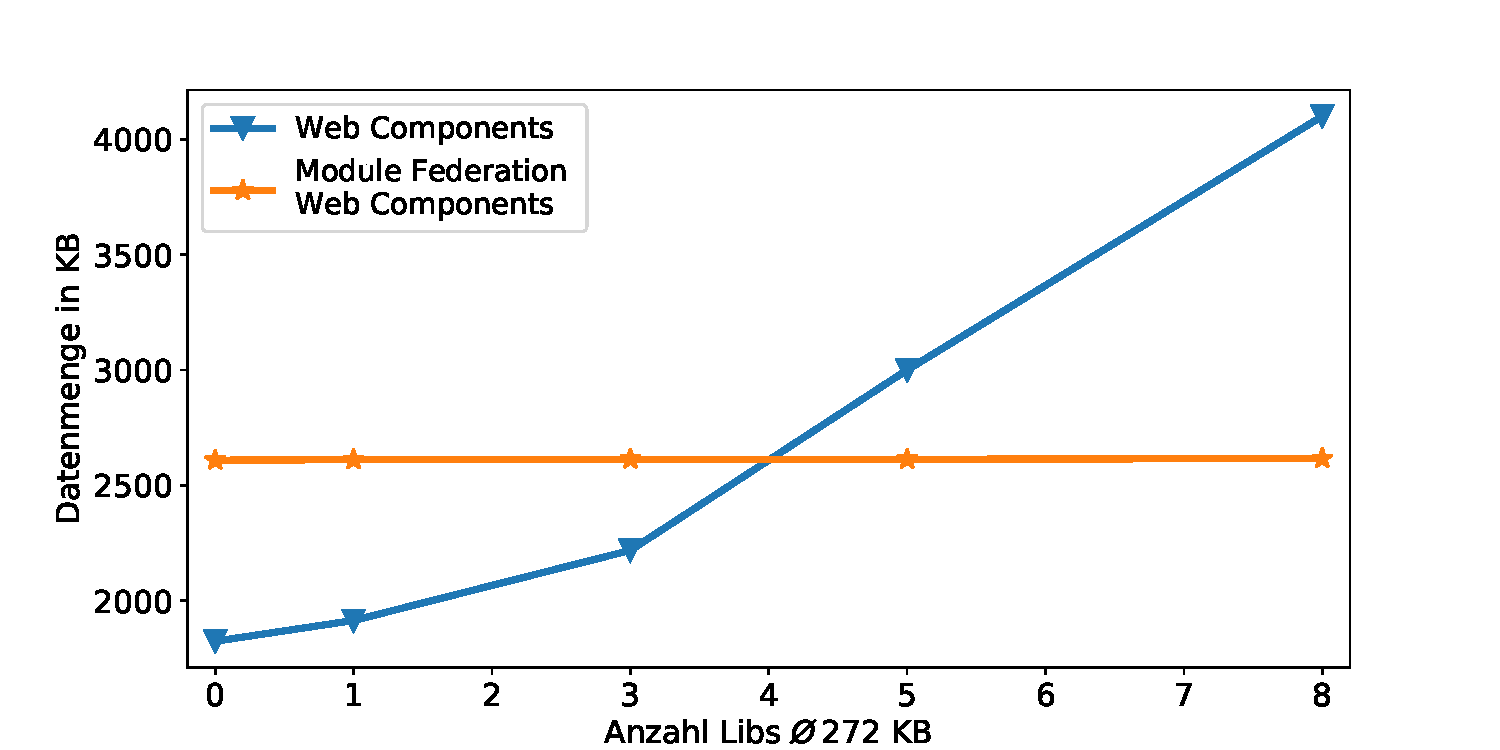
\includegraphics[width=1\textwidth]{img/appendix/DatasizeEval/MFWCvsMF_Datasize}}\\ % Pfad
		\source{Eigene Darstellung} % Quelle
		\label{fig:DatenmengeMFWC-WC}
	\end{minipage}
\end{figure}

Es wurden 5 Messungen mit null, einer, drei, fünf und acht verwendeten Bibliotheken durchgeführt. In \cref{fig:GGMessungBibs} in Anhang \ref{app:Bilder} sind die Bibliotheken pro Messlauf mit der durchschnittlichen Paketgröße dargestellt. Die vorherige \cref{fig:DatenmengeMFWC-WC} zeigt, dass ab 800\gls{KB}, welche durch Bibliotheken übertragen werden, Module Federation die bessere Art der Einbindung ist, um übertragene Datenmengen einzusparen. Die blaue Linie der Web Components Datenmenge weist einen leichten Knick am dritten Messpunkt auf, weil die eingebundenen Bibliotheken nicht alle genau dem Durchschnitt entsprechen.\footnote{Vgl. \cref{fig:GGMessungBibs} in Anhang \ref{app:Bilder}} Wären sie alle gleich groß, so würde der Graph linear verlaufen.

Allerdings ist das Teilen von Bibliotheken nur von Vorteil, wenn die Bibliothek ohnehin schon von der Portalshell geladen werden musste. Dies ist beispielsweise bei Standardbibliotheken wie \textit{@angular/core} oder einer geteilten Fachbibliothek, welche sowohl Microfrontend als auch die Portalshell benötigen, der Fall. Ebenfalls ist es auch vorstellbar, dass mehrere Microfrontends die gleiche Bibliothek benötigen, die Portalshell aber ursprünglich nicht. Dann könnte die Portalshell so umgebaut werden, dass die mehrfach benötigten Bibliotheken einmalig von der Portalshell eingebunden werden und sämtliche Microfrontends dann auf die eine eingebundene Bibliothek zugreifen, um Datenmenge zu sparen.

Module Federation kann gegenüber Web Components oder einem Iframe Vorteile bei der übertragenen Datenmenge bringen, jedoch nur im besonderen Anwendungsfall. Bei kleinen Microfrontends ohne abhängigen Bibliotheken sind Iframes und Web Components im Vorteil. Bei großen Lösungen mit vielen Bibliotheken, lohnt sich die Einbindung über Module Federation wiederum.

Das Kriterium \textit{Datenmenge} mit einer Gewichtung von 1,52\% wird daher mit 4 von 5 Punkten bewertet und erhält somit einen Teilnutzwert von 0,0608.

\textbf{Zwischenfazit}\\
Module Federation mit Web Components überträgt die Vorteile der Module Federation Einbindung von Angular Modulen auf andere Web Frameworks. Dadurch ist die Kompatibilität gegenüber anderen Frameworks hoch. Ebenfalls positiv anzumerken sind geringe Renderingzeiten sowie die Reduzierung der übertragenen Datenmenge, besonders bei geeigneten Konstellationen. Module Federation mit Web Components hat von den vier verglichenen Arten der Einbindung den höchsten Einrichtungsaufwand und ist ebenfalls kein offiziell anerkannter Standard von Angular.

\subsection{Vergleich der Arten untereinander}\label{sec:VergleichDerArten}

In diesem Abschnitt werden die im vorherigen Kapitel \cref{sec:AnalyseVerschiedenerIntegrationsansaetze} festgestellten Ausprägungen für jedes Kriterium jeder Alternative miteinander verglichen, um somit die beste Lösung für jedes Kriterium festzustellen.

In der nachfolgenden \cref{fig:ErgebnisNWA} sind die einzelnen Teilnutzwerte je Art der Einbindung und Kriterium in einer Tabelle gegenübergestellt. Die Teilnutzwerte sind gruppiert pro Kriterium in einer Farbskala dargestellt, damit der höchste Teilnutzwert (in grün) je Kriterium erkennbar ist.

\newpage
\begin{figure}[hbt!]
	\begin{minipage}[t]{1\textwidth}	
		\caption{Gegenüberstellung Ergebnisse der Nutzwertanalyse}
		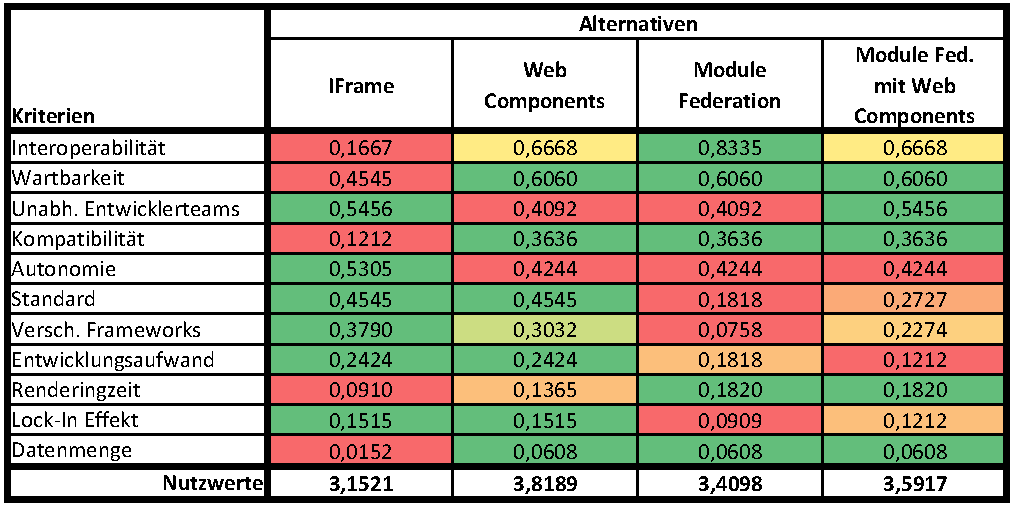
\includegraphics[width=1\textwidth]{img/ErgebnisNWA}\\ % Pfad
		\source{Eigene Darstellung} % Quelle
		\label{fig:ErgebnisNWA}
	\end{minipage}
\end{figure}

Für den gegebenen Anwendungsfall hat die Web Component bei der Evaluierung den höchsten Nutzwert erreicht. Dennoch konnten Web Components nicht bei allen Kriterien den höchsten Teilnutzwert erzielen, denn die direkte Gegenüberstellung der Einbindungsarten zeigt, dass keine der vier Arten für alle elf Kriterien am besten geeignet ist. 

Dies lässt darauf schließen, dass die Arten der Einbindung abhängig nach ihrem gegebenen Anwendungsfall optimal sind. Eine Übersicht, welche Art der Einbindung bei welchem Anwendungsfall optimal geeignet ist, wird im nachfolgenden \cref{sec:OptimaleAnwendungsszenarien} dargestellt.

\subsection{Optimale Anwendungsszenarien je nach Art der Einbindung}\label{sec:OptimaleAnwendungsszenarien}

In diesem Abschnitt werden Anwendungsszenarien mit den dazugehörigen Problemstellungen den Kriterien zugeteilt, danach mit den Arten der Einbindung verglichen und auf Basis der Ergebnisse ein Entscheidungsleitfaden gebildet.

Die nachfolgende \cref{tab:AnwendungsfallZuKriterium} zeigt vier Anwendungsfälle, welche verschiedene Problemstellungen aufweisen und dadurch unterschiedlich viel Wert auf einzelne Kriterien legen.

\begin{table}[!hbt]
	\centering
	\begin{minipage}[t]{1\textwidth}	
		\caption{Zusammenhang Kriterium zu Anwendungsfall} % Überschrift
		\begin{tabularx}{\columnwidth}{| c || X | c |}
			\toprule
			\thead{\textbf{Anwendungsfall}} & \thead{\textbf{Beispielhafte Problemstellung}} & \thead{\textbf{Kriterien}} \\
			\midrule
			Legacy Applikation & \makecell{Veraltete Frameworks,\\wenig KnowHow,\\keine Investition,\\Kundenanforderung} & \makecell{Entwicklungsaufwand,\\Kompatibilität} \\
			\midrule
			\makecell{Moderne Applikation,\\geringer Umfang} & \makecell{ReactJS als Framework,\\geringe Datenmenge nötig,\\Komplexität} & \makecell{Datenmenge,\\Frameworks}\\
			\midrule
			\makecell{Moderne Applikation,\\mittlerer Umfang}  & \makecell{Wiederverwendbar,\\Neuentwicklung, universell,\\Interoperabilität} & \makecell{Entwicklungsaufwand,\\Frameworks} \\
			\midrule
			\makecell{Moderne Applikation,\\großer Umfang} & \makecell{Angular als Framework,\\viel Routing,\\große Bibliotheken} & \makecell{Interoperabilität,\\Kompatibilität,\\ Datenmenge} \\
			\bottomrule
		\end{tabularx}
		\source{Eigene Darstellung}
		\label{tab:AnwendungsfallZuKriterium}
	\end{minipage}
\end{table}

Für vier Anwendungsfälle muss die jeweils beste Lösung zur Einbindung in die Portalshell gefunden werden. Dafür wird ein Entscheidungsbaum erstellt, welcher sich an dem von Geers im Grundlagenteil der Thesis in \cref{fig:EntscheidungsbaumArchitektur} orientiert, aber auf den Prototyp angepasst und durch die Erkenntnisse aus \cref{fig:ErgebnisNWA} optimiert ist. Der entwickelte Entscheidungsbaum ist in der nachfolgenden \cref{fig:Entscheidungsbaum} für Microfrontends zur Einbindung in eine Angular Portalapplikation dargestellt.

\newpage
\begin{figure}[hbt!]
	\centering
	\begin{minipage}[t]{0.95\textwidth}	
		\caption{Entscheidungsbaum: Einbindung Microfrontend in Portalshell}
		\frame{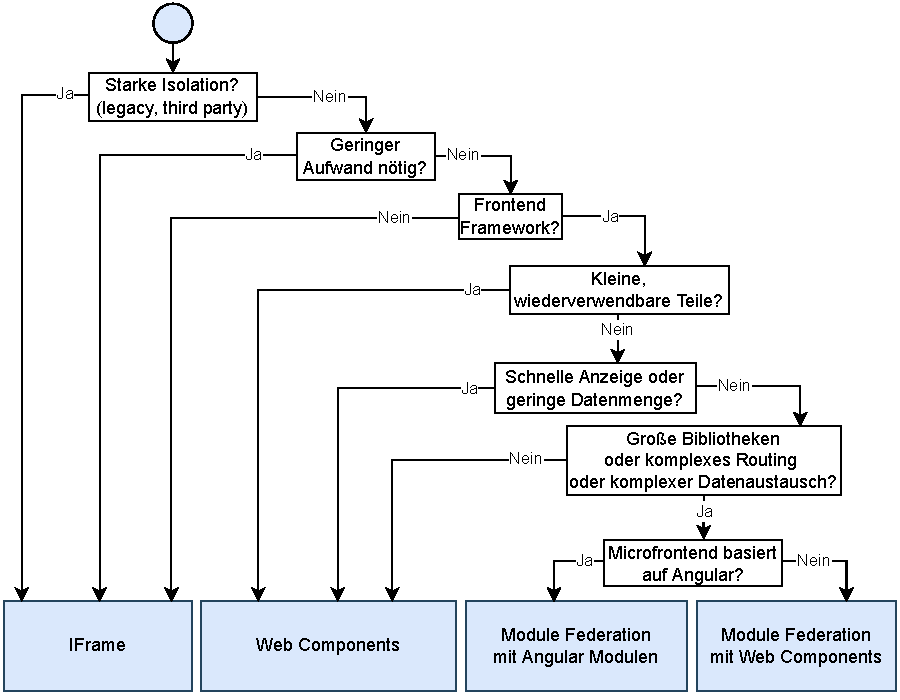
\includegraphics[width=1\textwidth]{img/Entscheidungsbaum}}\\ % Pfad
		\source{Eigene Darstellung} % Quelle
		\label{fig:Entscheidungsbaum}
	\end{minipage}
\end{figure}

Die Nutzwertanalyse hat ergeben, dass Iframes sich gut eignen, wenn Microfrontends eingebunden werden sollen, die Altlasten sind, nicht viel Aufwand erzeugen sollen, kein Web Frontend Framework enthalten oder stark gegen andere Microfrontends isoliert werden müssen. 

Ist der Use-Case des Microfrontends klein und wiederverwendbar, bspw. die konfigurierbaren Anzeige eines \gls{KPI}, oder kommt es auf schnelle Anzeige oder geringe übertragene Datenmenge bei wenig Bibliotheken an, so sind Web Components zu empfehlen.

Bei großer Datenmenge durch Bibliotheken, bei komplexem Routing im Microfrontend oder intensivem Datenaustausch mit der Portalshell empfiehlt sich die Einbindung über Module Federation. Abhängig davon, ob das Web Framework des Microfrontends Angular ist, sollte Module Federation mit Web Components oder mit Angular Modulen gewählt werden.

%!TEX root = ../Thesis.tex
\section{Prototypische Implementierung}\label{sec:Implementierung}

In diesem Kapitel werden die Erkenntnisse aus dem vorherigen \cref{sec:Evaluierung} auf das prototypische Beispiel aus \cref{sec:PrototypischesBeispiel} angewendet. Dafür wird zunächst der Anpassungsbedarf an der Beispielapplikation erläutert, dann die Microfrontends eingebunden und anschließend zur Kontrolle des erstellten Prozesses die Ergebnisse validiert.

Die drei Microfrontends aus \cref{sec:PrototypischesBeispiel} (Wetter-App, Taschenrechner-App und Statistik-App) werden anhand des in \cref{fig:Entscheidungsbaum} dargestellten Entscheidungsbaumes der jeweiligen passenden Art der Einbindung zugewiesen.

Die Wetter-App soll für jeden Mandanten wiederverwendet und in einem \nobreak{Dashboard} mehrfach eingebunden werden können, damit das Wetter unterschiedlicher Städte angezeigt werden kann. Es handelt sich um eine Eigenentwicklung in Angular ohne große Komplexität und eigenes Routing. Daher wird sie über Web Components eingebunden.

Ein Taschenrechner ist online frei verfügbar abrufbar unter \url{https://www.blitzrechner.de/taschenrechner-wissenschaftlich/}. Dieser Rechner bildet sämtliche Funktionalitäten ab, sodass der Aufwand für eine Eigenentwicklung nicht gerechtfertigt wäre. Von daher wird der Taschenrechner des Drittanbieters als Iframe eingebunden.

Die Statistik-App ist eine Eigenentwicklung in Angular. Sie beinhaltet große Bibliotheken zum Darstellen von Graphen und Berechnen von Statistiken. Deswegen ist eine Einbindung über Module Federation mit Angular Modulen zu empfehlen. Die App teilt sich Bibliotheken mit der Portalshell und bekommt durch eine \texttt{AuthLib} Informationen über den User von der Portalapplikation, damit das Rechtekonzept umgesetzt werden kann.

\subsection{Anpassungsbedarf der Beispielapplikation}\label{sec:ImplementierungAnpassungsbedarf}

Bei der prototypischen Beispielapplikation aus \cref{sec:PrototypischesBeispiel} liegt Anpassungsbedarf nach den Erkenntnissen aus der vorangegangenen Evaluierung vor. Die Portalshell muss erweitert werden, sodass Microfrontends als Iframe, Web Component und Module Federation mit Angular Modulen eingebunden werden können. Die Portalshell sollte dafür eine Oberfläche bereitstellen, welche das Einbinden der Microfrontends dynamisch ermöglicht und die Konfiguration in einer Datenbank speichert. Auf das dynamische Einbinden und das Entwickeln einer Oberfläche zum Administrieren wird verzichtet, da dies den Rahmen eines Prototypen übersteigen würde. 

Allerdings wird die Portalshell um drei Komponenten erweitert, die das Einbinden von Microfrontends anhand der nötigen Parameter ermöglichen. So wird gezeigt, dass das Einbinden dynamisch geschehen könnte, wenn die Komponenten dynamisch vom Backend befüllt werden würden.

Das Designmockup aus \cref{fig:MockupBeispiel} in Anhang \ref{app:Bilder} sieht eine horizontale Trennung der Microfrontend-Architektur vor.\footnote{Siehe \cref{fig:HorizontalVerticalSplit}} So sind mehrere Microfrontends, die von verschiedenen Teams verwaltet werden, auf einem Dashboard eingebunden. Der Inhalt des angezeigten Dashboards besteht dann aus vier Microfrontendinstanzen von drei unterschiedlichen Microfrontend-Templates. Die Komponenten zum Einbinden der Microfrontendinstanzen geben das Styling zur Ausrichtung auf dem Dashboard vor.

\subsection{Implementierung der Microfrontends}\label{sec:ImplementierungEinbindungMicrofrontends}

Das Taschenrechner-Microfrontend konnte mit geringem Aufwand als Iframe eingebunden werden. Dadurch, dass der Taschenrechner bereits abrufbar zur Verfügung stand, wurde Entwicklungsaufwand vermieden. Für die Einbindung war es Ausreichend die \gls{URL} des Taschenrechner-Microfrontends mit Breite- und Höhe-Parametern an die \textit{Iframe-Injection-Komponente}\footnote{Sourcecode in Anhang \ref{app:Listing} in \cref{list:IFrameInjectionComponent}} der Portalshell zu übergeben. Das durch die \textit{Iframe-Injection-Komponente} generierte \gls{HTML} ist in Anhang \ref{app:Listing} in \cref{list:PrototypTaschenrechner} zu sehen.

Die Wetter-App wurde als Angular Komponente entwickelt und dann als Web Component exportiert. Statt wirklich eine Wetter-\gls{API} anzusprechen und die Wetterdaten des Standort-Parameters abzufragen, wird lediglich der Standort prototypisch angezeigt. Der Sourcecode der \textit{Weather-Component} ist in Anhang \ref{app:Listing} in \cref{list:SourceCodeWeatherComponent} dargestellt. Die Web Component wurde automatisch gebaut und die generierte \texttt{main.js}-Datei in einem Azure Storage Account abgelegt. 

Die Portalshell nimmt die \gls{URL} zur \texttt{main.js} entgegen und kann durch die \textit{WC-Injection-\linebreak Component}\footnote{Sourcecode in Anhang \ref{app:Listing} in \cref{list:WCInjectionComponent}} die \textit{Weather-Component} in den \gls{DOM}-Tree des Dashboards einbinden.

Die Statistik-App wurde selber entwickelt und über Module Federation in die Portalshell eingebunden. Dafür wurde die Routing-Konfiguration so angepasst, dass das Module Federation Microfrontend in ein zweites Router-Outlet mit dem Namen \textit{modulefederation} gerendert wird, welches in der Seite eingebunden ist (siehe \cref{list:EinbindungModuleFederation} in Anhang \ref{app:Listing}). Für jedes Module Federation Microfrontend, das über ein Angular Modul eingebunden wird, muss eine Route hinterlegt werden. Das Hinterlegen kann auch dynamisch mit übergebenen Variablen passieren.

Das Einbinden einer Web Component über Module Federation könnte mit einer \texttt{Module-\\Federation-WC-Injection}-Component geschehen, die den Code der geladenen Web Component in den \gls{DOM}-Tree des aktuellen Dashboards automatisch einfügt. Aber da die Portalshell und das Microfrontend beide in der aktuell neusten Angular Version entwickelt wurden, ist dies nicht notwendig.

\subsection{Validierung der Kriterien}\label{sec:ImplementierungValidierungKriterien}

In der nachfolgenden \cref{fig:ImplementierungScreenshot} ist die finale prototypische Implementierung der in \cref{sec:PrototypischesBeispiel} beschriebenen Beispielapplikation zu sehen. Da es sich um eine Implementierung mit Fokus auf der technischen Machbarkeit handelt, wurde das Design vernachlässigt. Dies könnte mit einem Bootstrap Theme\footnote{Siehe beispielsweise \url{https://themes.getbootstrap.com/}} einheitlich nachgezogen werden.

\newpage
\begin{figure}[hbt!]
	\begin{minipage}[t]{1\textwidth}	
		\caption{Prototypische Implementierung des Dashboard \textit{Prototyp}}
		\frame{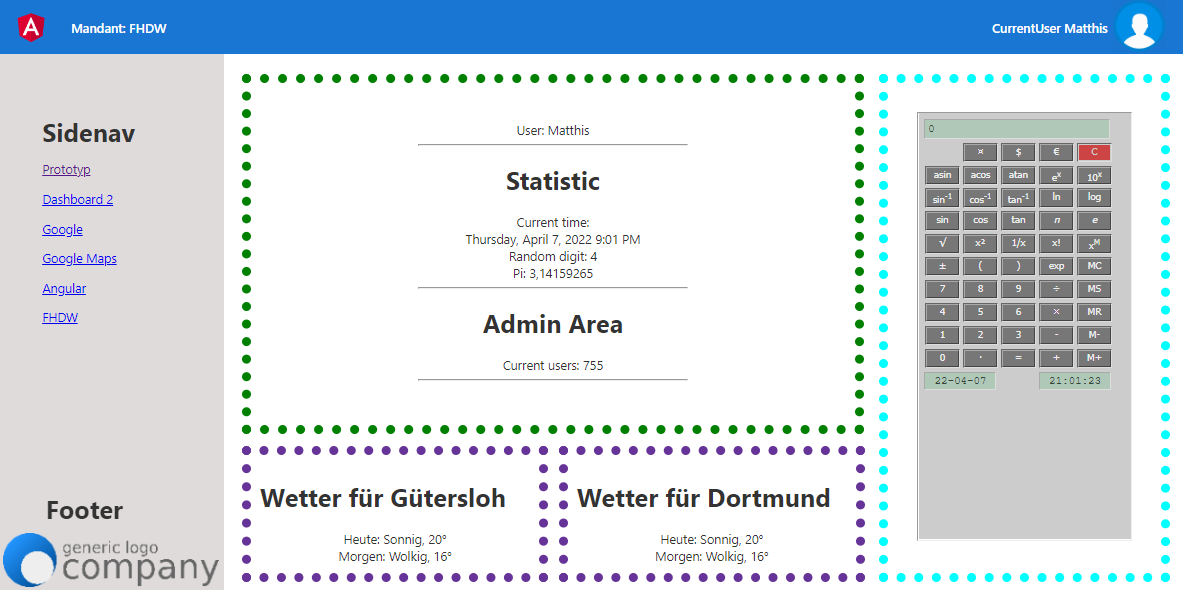
\includegraphics[width=1\textwidth]{img/PrototypMicrofrontends}}\\ % Pfad
		\source{Eigene Darstellung} % Quelle
		\label{fig:ImplementierungScreenshot}
	\end{minipage}
\end{figure}

Die implementierte Lösung gleicht dem Mockup aus \cref{fig:MockupBeispiel}, welche in \cref{sec:PrototypischesBeispiel} vorgestellt wurde. Die vier Microfrontendinstanzen sind nebeneinander dargestellt. Eine horizontale Trennung wurde ermöglicht, sodass mehrere Instanzen auf einer Seite dargestellt werden können. Die Microfrontends sind zur besseren Darstellung der Trennung mit einem farblichen Rahmen dargestellt.

Das Module Federation Microfrontend (grün) teilt einige seiner Bibliotheken mit der Portalshell. Zum jetzigen Zeitpunkt wird dadurch kaum Datenmenge eingespart. Aber wenn weitere Statistik-Apps eingebunden werden würden, würden diese von der Teilung der Bibliotheken profitieren. Die Statistik-App kann ihr Rechtekonzept anwenden. Sie bezieht die Informationen des angemeldeten Benutzers aus einer mit der Portalshell geteilten \texttt{AuthLib}\footnote{\cite[Sourcecode unter][]{Steyer2021f}}. Die \texttt{AuthLib} wird beim Login mit den Userdaten gefüllt und Module Federation Microfrontends können sie einbinden und Daten konsumieren.

Die geteilten Userinformationen (Benutzername: \textit{Matthis}) sind sowohl im Microfrontend, als auch im Header der Portalshell dargestellt und werden beide Male dynamisch aus der \texttt{AuthLib} bezogen. Da der User \textit{Matthis} die Rolle Admin zugeordnet hat, sieht er den erweiterten Admin-Bereich in der Statistik-App. Andere Komponenten können ebenfalls Daten aus der \texttt{AuthLib} konsumieren.

Die Wetter-App (lila) wurde doppelt mit unterschiedlichen Standorten als Web Component eingebunden. So konnte die Komponente nach einmaligem Einbinden wiederverwendet werden, ohne ein zweites Mal zum Client geladen zu werden.\footnote{Siehe \cref{fig:PrototypEinmaligesLadenWC} in Anhang \ref{app:Bilder}}

Das Taschenrechner Microfrontend (blau) konnte von \url{https://www.blitzrechner.de/taschenrechner-wissenschaftlich/} als Iframe eingebunden werden. Der benötigte Aufwand zum Einbinden der verschiedenen Arten skalierte mit den geschätzten Erkenntnissen des Aufwands von \cref{tab:MessungenEvaluierung} aus \cref{sec:EvaluierungIFrame} und war dementsprechend gering.

\textbf{Fazit}\\
Der in \cref{sec:Evaluierung} durch die Nutzwertanalyse entwickelte Entscheidungsbaum konnte an den Microfrontends des prototypischen Beispieles durchlaufen werden. Die Microfrontends wurden dadurch jeweils nach der geeignetsten Art in die Portalshell eingebunden. Durch die Erkenntnisse aus \cref{sec:ImplementierungValidierungKriterien} konnte bestätigt werden, dass der entwickelte Entscheidungsbaum anwendbar ist und sinnvolle Resultate erzielt.

%!TEX root = ../Thesis.tex
\section{Schlussbetrachtung}\label{sec:Schlussbetrachtung}

In diesem Kapitel wird eine Schlussbetrachtung zu der erstellten \dokumententyp{} durchgeführt. Dafür wird im nachfolgenden Abschnitt ein Fazit über die Erkenntnisse erstellt und im darauffolgenden \cref{sec:Ausblick} potentielle weitere Themen erläutert, welche noch weiterführend betrachtet werden könnten.

\subsection{Zusammenfassung}\label{sec:Fazit}

Ziel der Arbeit war es, eine differenzierte Entscheidungshilfe zu erstellen, anhand derer die optimale Art der Einbindung von Microfrontends in eine Portalshell ermittelt werden kann.

Es wurde die Erkenntnis gesammelt, dass Web Components den größten Nutzwert im Vergleich der Einbindungsarten untereinander erreichen. Allerdings schneiden Web Components in einigen Kriterien schlechter ab, als andere Arten der Einbindung. Jede der vier Einbindungsarten konnte bei mindestens fünf Kriterien den höchsten Teilnutzwert erreichen. Dies zeigt, dass eine Einzelfallbetrachtung basierend auf den individuellen Anforderungen jedes Microfrontends durchgeführt werden muss, um die optimale Art der Einbindung in eine Portalshell bestimmen zu können. Dafür wurde eine Entscheidungshilfe in Form eines Entscheidungsbaumes im letzten \cref{sec:OptimaleAnwendungsszenarien} der Nutzwertanalyse erstellt. 

Durch den in \cref{sec:PrototypischesBeispiel} beschriebenen Prototypen wurden die Erkenntnisse der Nutzwertanalyse auf die zutreffenden individuellen Ansprüche des Prototypen und dessen Microfrontends angepasst. Im vorletzten \cref{sec:Implementierung} \textit{Prototypische Implementierung} wurde das Ergebnis der Nutzwertanalyse und der daraus entstandene Entscheidungsbaum angewendet und überprüft. Es stellte sich heraus, dass die prototypische Portalshell von den Erkenntnissen profitieren konnte und die verschiedenen Arten der Einbindung ihre Vorteile an den Microfrontends anwenden konnten.

\subsection{Ausblick}\label{sec:Ausblick}

Die Frontend-Entwicklung sowie die Softwarearchitektur sind umfangreiche Themengebiete. Es gibt noch weitere Optionen, welche tiefer untersucht und eingebracht werden könnten.

Zu diesen Themen zählt beispielsweise die Ermittlung von optimalen Hostingszenarien für Microfrontends. Es könnte On-Premise Hosting mit dem Hosting bei Cloud Service Providern verglichen werden. Ein weiterer möglicher Blickwinkel wäre der Vergleich verschiedener Cloud Hosting Optionen untereinander. So könnten im Kubernetes-Cluster gehostete Microfrontends gegenüber Microfrontends gehostet in einer \gls{VM} gegenüber Hosting in einer \textit{\gls{PaaS}}-Lösung eines Cloud-Anbieters zu diversen Kriterien (bspw. Kosten, Ausfallsicherheit, Unabhängigkeit und Skalierbarkeit) verglichen werden.

Ebenfalls könnte das Konzept eines Design Systems näher untersucht werden. Ein einheitliches Design in verteilten, autonomen Teams durchzusetzen, ist nicht trivial, kann aber viele Vorteile für die Entwickler sowie die Benutzer der Applikation bringen. Michael Geers gibt im zwölften Kapitel seines Buches \textit{Micro Frontends in Action} Denkanstöße und Sichtweisen, welche Potential für eine wissenschaftliche Aufarbeitung bieten.\footnote{\cite[vgl.][213]{Geers2020}}

Das Konzept einer Portalshell wurde im Rahmen der \dokumententyp{} nur prototypisch beschrieben und umgesetzt. Eine mandantenfähige Portalshell basierend auf einer dynamischen Microfrontend-Architektur hat das Potential die Softwarelösungen für eine ganze Branche abzubilden. Dafür müssten allerdings aufwändige Prozesse entwickelt und umgesetzt werden. Dies würde von dynamischer Instanziierung der Microfrontends je Mandant mit automatisiertem Deployment bis hin zu der Erstellung eines zentralen Monitoring- sowie Abrechnungskonzeptes reichen.
	
%%%%%%%%%%%%%%%%%%%%%%%%%%%%%%%%%%%%%%%%%%%%%%%%%%%%%%%%%%%%%%%%%%%%%%%

%!TEX root = ../Thesis.tex
\section*{Anhang}
\addcontentsline{toc}{section}{Anhang}
\fancyhead[R]{Anhang}

\anhangsverzeichnis

\anhang{Listings}\label{app:Listing}

\begin{figure}[bht]
	\begin{lstlisting}[caption=Exemplarische Konfiguration Module Federation Portalshell, label=lst:ModuleFederationWebpackShell, language=Javascript]
		[...]
		plugins: [
		new ModuleFederationPlugin({
			
			remotes: {
				"microapp": "microapp@http://localhost:3000/remoteEntry.js",
			},
			shared: share({
				"@angular/core": { singleton: true, strictVersion: true, requiredVersion: 'auto' }, 
				"@angular/common": { singleton: true, strictVersion: true, requiredVersion: 'auto' }, 
				"@angular/common/http": { singleton: true, strictVersion: true, requiredVersion: 'auto' }, 
				"@angular/router": { singleton: true, strictVersion: true, requiredVersion: 'auto' },
				
				...sharedMappings.getDescriptors()
			})
			
		}),
		sharedMappings.getPlugin()
		],
		[...]
	\end{lstlisting}
	\footnoterule{}
	\footnotesize{Auszug aus der \texttt{webpack.config.js} einer Portalshell}
\end{figure}

\newpage
\begin{figure}[bht]
	\begin{lstlisting}[caption=Exemplarische Konfiguration Module Federation Microfrontend, label=lst:ModuleFederationWebpackRemote, language=Javascript]
		[...]
		plugins: [
		new ModuleFederationPlugin({      
			name: "microapp",
			filename: "remoteEntry.js",  
			exposes: {
				'./Module': './src/app/distant/distant.module.ts',
			},
			shared: share({
				"@angular/core": { singleton: true, strictVersion: true, requiredVersion: 'auto' }, 
				"@angular/common": { singleton: true, strictVersion: true, requiredVersion: 'auto' }, 
				"@angular/common/http": { singleton: true, strictVersion: true, requiredVersion: 'auto' }, 
				"@angular/router": { singleton: true, strictVersion: true, requiredVersion: 'auto' },
				
				...sharedMappings.getDescriptors()
			})        
		}),
		sharedMappings.getPlugin()
		],
		[...]
	\end{lstlisting}
	\footnoterule{}
	\footnotesize{Auszug aus der \texttt{webpack.config.js} eines Microfrontends}
\end{figure}

\newpage
\begin{figure}[bht]
	\begin{lstlisting}[caption=Konfiguration eines Module Federation Microfrontends, label=lst:WebpackConfigMF, language=Javascript]
		[...]
		plugins: [
		new ModuleFederationPlugin({
			library: { type: "module" },
			
			name: "evalmf",
			filename: "remoteEntry.js",
			exposes: {
				'./Module': './src/app/export/export.module.ts',
			},   
			
			shared: share({
				"@angular/core": { singleton: true, strictVersion: true, requiredVersion: 'auto' }, 
				"@angular/common": { singleton: true, strictVersion: true, requiredVersion: 'auto' }, 
				"@angular/common/http": { singleton: true, strictVersion: true,	requiredVersion: 'auto' }, 
				"@angular/router": { singleton: true, strictVersion: true, requiredVersion: 'auto' },
				"@angular/material": { singleton: true, strictVersion: true, requiredVersion: 'auto' },
				
				...sharedMappings.getDescriptors()
			})
			
		}),
		sharedMappings.getPlugin()
		],
		[...]
	\end{lstlisting}
	\footnoterule{}
	\footnotesize{Auszug aus der \texttt{webpack.config.js} eines Microfrontends}
\end{figure}

\newpage
\begin{figure}[bht]
	\begin{lstlisting}[caption=Konfiguration einer Module Federation Portalshell, label=lst:WebpackConfigPS, language=Javascript]	
		[...]
		plugins: [
		new ModuleFederationPlugin({
			library: { type: "module" },
			shared: share({
				"@angular/core": { singleton: true, strictVersion: true, requiredVersion: 'auto' }, 
				"@angular/common": { singleton: true, strictVersion: true, requiredVersion: 'auto' }, 
				"@angular/common/http": { singleton: true, strictVersion: true,	requiredVersion: 'auto' }, 
				"@angular/router": { singleton: true, strictVersion: true, requiredVersion: 'auto' },
				"@angular/material": { singleton: true, strictVersion: true, requiredVersion: 'auto' },
				
				...sharedMappings.getDescriptors()
			})
			
		}),
		sharedMappings.getPlugin()
		],
		[...]
	\end{lstlisting}
	\footnoterule{}
	\footnotesize{Auszug aus der \texttt{webpack.config.js} der Portalshell}
\end{figure}

\newpage
\begin{figure}[bht]
	\begin{lstlisting}[caption=Einbindung eines Module Federation Microfrontend, label=lst:MFPSConfig2, language=Javascript]
		// decl.d.ts
		declare module 'evalmf/Module';
		
		// app.routes.ts
		const URL = 'http://localhost:4202/remoteEntry.js';
		{
			path: 'EvalMF',
			loadChildren: () => loadRemoteModule({
				type: 'module',
				remoteEntry: URL,
				exposedModule: './Module'
			})
			.then(m => m.ExportModule) 
		},
	\end{lstlisting}
	\footnoterule{}
	\footnotesize{Auszüge aus der \texttt{decl.d.ts} und \texttt{app.routes.ts} der Portalshell}
\end{figure}

\newpage
\begin{figure}[bht]
	\begin{lstlisting}[caption=Konfiguration von Module Federation mit Web Components, label=lst:WebpackConfigMFWC, language=Javascript]
		[...]	
		plugins: [
		new ModuleFederationPlugin({
			name: "evalmfwc",
			library: { type: "var", name: "evalmfwc" },
			filename: "remoteEntry.js",
			exposes: {
				'./web-components': './src/bootstrap.ts',
			},        
			
			shared: share({
				"@angular/core": { singleton: true, strictVersion: true,requiredVersion: 'auto' }, 
				"@angular/common": { singleton: true, strictVersion: true, requiredVersion: 'auto' }, 
				"@angular/common/http": { singleton: true, strictVersion: true, requiredVersion: 'auto' }, 
				"@angular/router": { singleton: true, strictVersion: true, requiredVersion: 'auto' },
				"@angular/material": { singleton: true, strictVersion: true, requiredVersion: 'auto' },
				
				...sharedMappings.getDescriptors()
			})
		})
		],
		[...]
	\end{lstlisting}
	\footnoterule{}
	\footnotesize{Auszug aus der \texttt{webpack.config.js} eines Microfrontends}
\end{figure}

\newpage
\begin{figure}[bht]
	\begin{lstlisting}[caption=Definition des customElements zur Einbindung als Web Component, label=lst:MFWCAppModule, language=Javascript]
		[...]
		ngDoBootstrap() {
			const webComponent = createCustomElement(ContentComponent, {injector: this.injector});
			//avoid double registration errors
			if(!customElements.get('content-component-mf')){
				customElements.define('content-component-mf', webComponent);
			}
		}
		[...]
	\end{lstlisting}
	\footnoterule{}
	\footnotesize{Auszug aus der \texttt{app.module.ts} des Microfrontends}
\end{figure}

\newpage
\begin{figure}[bht]
	\begin{lstlisting}[caption=Laden einer Web Component durch Module Federation, label=lst:MFPSWCConfig2, language=Javascript]
		// decl.d.ts
		declare module 'evalmfwc/web-components';
		
		// registry.ts
		export const registry = {
			evalmfwc: () => loadRemoteModule({
				type: 'script',
				remoteEntry: 'http://localhost:4204/remoteEntry.js',
				remoteName: 'evalmfwc',
				exposedModule: './web-components'
			})
		};
	
		// app.routes.ts - Portalshell
		[...]
		{
			path: 'EvalMFWC',
			component: WrapperComponent,
			pathMatch: 'full', 
			data: { importName: 'evalwcmf', elementName: 'content-component-mf' }
		},
		[...]
	\end{lstlisting}
	\footnoterule{}
	\footnotesize{Inhalte der \texttt{decl.d.ts}, \texttt{registry.ts} und Ausschnitte der \texttt{app.routes.ts} einer Portalshell}
\end{figure}

\newpage
\begin{figure}[bht]
	\begin{lstlisting}[caption=Einbindung einer Web Component durch Module Federation, label=lst:MFPSWCWrapper, language=Javascript]
		@Component({
			template: '<div #vc></div>',
		})
		export class WrapperComponent implements AfterContentInit {
			
			@ViewChild('vc', {read: ElementRef, static: true})
			vc: ElementRef;
			
			constructor(private route: ActivatedRoute) { }
			
			ngAfterContentInit(): void {
				const elementName = this.route.snapshot.data.elementName;
				const importName = this.route.snapshot.data.importName;
	
				const importFn = registry[importName];
				importFn()
					.then(_ => console.debug(`element ${elementName} loaded!`))
					.catch(err => console.error(`error loading ${elementName}:`, err));
				
				const element = document.createElement(elementName);
				this.vc.nativeElement.appendChild(element);
			}
		}
	\end{lstlisting}
	\footnoterule{}
	\footnotesize{Inhalt der \texttt{wrapper.component.ts} der Portalshell}
\end{figure}

\begin{figure}[bht]
	\begin{lstlisting}[caption=Platzhalter für SSI, label=list:SSIPlaceholder]
		<!--#include virtual="/url/to/include" -->
	\end{lstlisting}
	\footnoterule{}
	\footnotesize{\textbf{Quelle:} \cite[][61]{Geers2020}}
\end{figure}

\newpage
\begin{figure}[bht]
	\begin{lstlisting}[caption=Nutzung eines HTML Templates, label=list:HTMLTemplate, language=Javascript]
		<button onclick="showContent()">Show hidden content</button>
		
		<template>
		<h2>Flower</h2>
		<img src="img_white_flower.jpg" width="214" height="204">
		</template>
		
		<script>
		function showContent() {
			var temp = document.getElementsByTagName("template")[0];
			var clon = temp.content.cloneNode(true);
			document.body.appendChild(clon);
		}
		</script>
	\end{lstlisting}
	\footnoterule{}
	\footnotesize{\textbf{Quelle:} \cite[][]{W3Schools2022}}
\end{figure}

\newpage
\begin{figure}[bht]
	\begin{lstlisting}[caption=Einbindung eines Taschenrechner als Iframe, label=list:PrototypTaschenrechner]
		[...]
		<iframe id="iframeId" src="https://www.blitzrechner.de/calculations/zf2Calculator/zf20.htm" name="Taschenrechner" 
		width="220" height="310" style="border: none"></iframe>
		[...]
	\end{lstlisting}
	\footnoterule{}
	\footnotesize{Auszug aus dem generierten HTML des Dashboard \textit{Prototyp}}
\end{figure}

\begin{figure}[bht]
	\begin{lstlisting}[caption=Quellcode der IframeInjection-Component, label=list:IFrameInjectionComponent, language=Javascript]
		import { Component, Input, OnInit } from '@angular/core';
		import * as $ from "jquery";
		
		@Component({
			selector: 'iframe-injection',
			template: '<iframe id="iframeId" [height]="height" [width]="width"></iframe>'
		})
		export class IframeInjectionComponent implements OnInit {
			
			@Input()
			url: string = '';
			@Input()
			height: string = '';
			@Input()
			width: string = '';
			
			ngOnInit(): void {
				$('#iframeId').attr('src', this.url);
			}
		}
	\end{lstlisting}
	\footnoterule{}
	\footnotesize{Inhalt der \texttt{Iframe-injection.component.ts} der Portalshell}
\end{figure}

\newpage
\begin{figure}[bht]
	\begin{lstlisting}[caption=Komponente zur Einbindung von Web Components, label=list:WCInjectionComponent, language=Javascript]
		import { Component, ElementRef, Input, OnInit } from '@angular/core';
		
		@Component({
			selector: 'web-component-injector',
			template: '',
		})
		export class WebComponentInjectorComponent implements OnInit {
			private element: HTMLElement;
			
			@Input() url: string = '';
			@Input() name: string = '';
			@Input() location: string = '';
			
			constructor(private wrapperElement: ElementRef) { }
			
			ngOnInit(): void {
				this.element = this.loadWCFromUrl(this.wrapperElement, this.url, this.name );
			}
			
			loadWCFromUrl(wrapper: ElementRef, hostingURL: string, htmlTagName: string) : HTMLElement {
				const wrapperElement: HTMLElement = wrapper.nativeElement;
				const shadow = wrapperElement.attachShadow({mode: 'open'});
				const script = document.createElement('script');
				script.src = hostingURL;
				
				const webComponent = document.createElement(htmlTagName);
				webComponent.setAttribute('location', this.location);
				
				script.onload = () => { shadow.appendChild(webComponent); }
				
				shadow.appendChild(script);
				return webComponent;
			}
		}
	\end{lstlisting}
	\footnoterule{}
	\footnotesize{Inhalt der \texttt{web-component-injector.component.ts} der Portalshell}
\end{figure}

\newpage
\begin{figure}[bht]
	\begin{lstlisting}[caption=Quellcode der Weather-Component, label=list:SourceCodeWeatherComponent, language=Javascript]
		import { Component, Input, ViewEncapsulation } from '@angular/core';
		
		@Component({
			selector: 'app-weather',
			template: `
			<div class="wrapper">
				<h1>Wetter fuer {{location}}</h1>
				<div class="center">
					<div>
						<label>Heute: Sonnig, 20 Grad</label>
					</div>
					<div>
						<label>Morgen: Wolkig, 16 Grad</label>
					</div>
				</div>
			</div>`,
			styles: ['.wrapper{width: 300px;margin: auto;}', '.center{display: inline;float: none;text-align: center;}'],
			encapsulation: ViewEncapsulation.ShadowDom
		})
		export class WeatherComponent {
			
			@Input()
			location: string = '';
			
		}
	\end{lstlisting}
	\footnoterule{}
	\footnotesize{Inhalt der \texttt{weather.component.ts} des Wetter-Microfrontends}
\end{figure}

\newpage
\begin{figure}[bht]
	\begin{lstlisting}[caption=Einbindung des Module Federation Microfrontends, label=list:EinbindungModuleFederation, language=Javascript]
		// app.routes.ts
		[...]
		{
			path: 'Prototyp',
			component: PrototypComponent,
			pathMatch: 'full',
			children: [
			{
				path: '', 
				outlet: 'modulefederation',
				loadChildren: () => loadRemoteModule({
					type: 'module',
					remoteEntry: URL,
					exposedModule: './Module'
				})
				.then(m => m.ExportModule)
			} ]
		},
		[...]
	
		// prototyp.component.html		
		[...]
		<div class="linksoben">
			<router-outlet name="modulefederation"></router-outlet>
		</div>		
		[...]
	\end{lstlisting}
	\footnoterule{}
	\footnotesize{Auszüge der \texttt{app.routes.ts} und \texttt{prototyp.component.html} der Portalshell}
\end{figure}

\newpage
\begin{figure}[bht]
	\begin{lstlisting}[caption=Einbindung einer Content-Component als Web Component, label=list:SelbstEinbindenWC]
		<!doctype html>
		<html lang="en">
		<head>
			<meta charset="utf-8">
			<title>WebComponent</title>
			<base href="/">
			[...]
		</head>
			<body class="mat-typography">
				<content-component></content-component>
			</body>
		</html>
	\end{lstlisting}
	\footnoterule{}
	\footnotesize{Auszüge der \texttt{index.html} des Web Component Microfrontends}
\end{figure}

\newpage
\anhang{Bilder}\label{app:Bilder}

\begin{figure}[hbt!]
	\centering
	\begin{minipage}[t]{0.9\textwidth}	
		\caption{Technologien für API Entwickler, Stand 07/2020}
		\frame{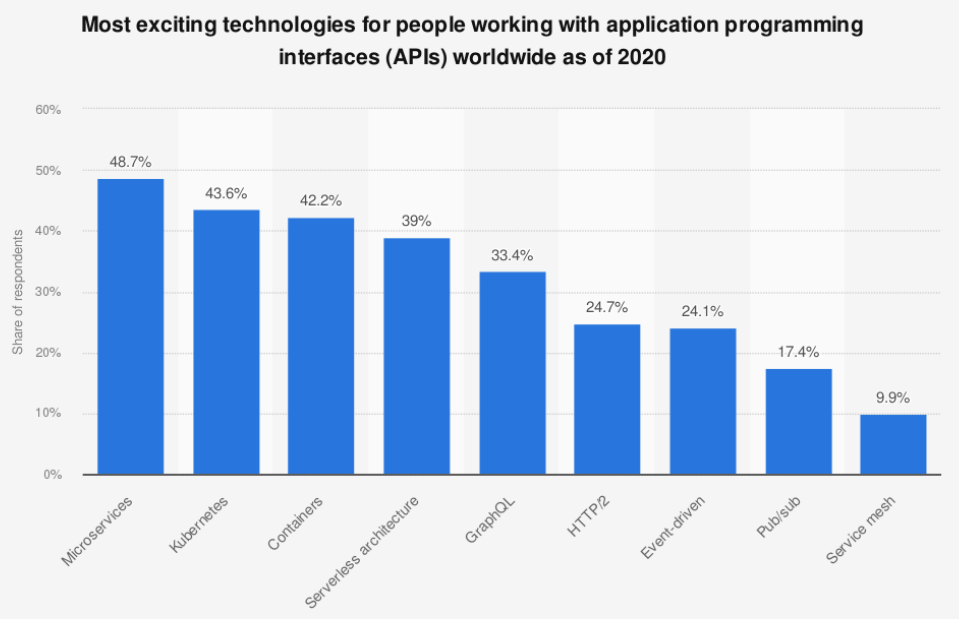
\includegraphics[width=1\textwidth]{img/appendix/StatistikMicroServices}}\\ % Pfad
		\source{\cite[][]{Statista2020a}} % Quelle
		\label{fig:StatistikMicroServices}
	\end{minipage}
\end{figure}

\begin{figure}[hbt!]
	\centering
	\begin{minipage}[t]{0.6\textwidth}	
		\caption{Konkrete Solutionarchitektur Beispielapplikation}
		\frame{\includegraphics[width=1\textwidth,page=3]{img/Beispielapplikation_Diagramm}}\\ % Pfad
		\source{Eigene Darstellung} % Quelle
		\label{fig:SolutionarchitekturBeispielapplikationKonkret}
	\end{minipage}
\end{figure}

\newpage
\begin{figure}[hbt!]
	\centering
	\begin{minipage}[t]{0.7\textwidth}	
		\caption{Vergleichbares Microfrontend für Evaluierung}
		\frame{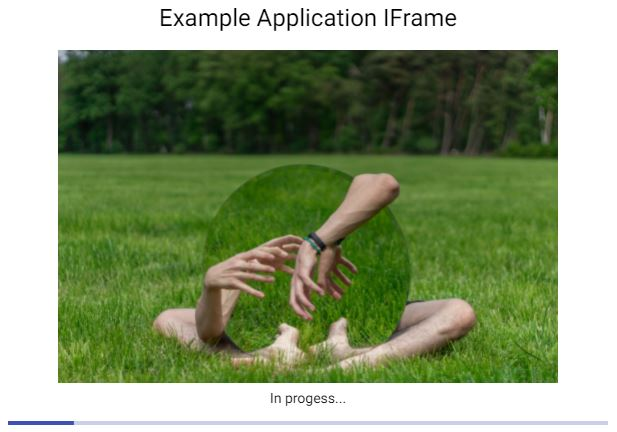
\includegraphics[width=1\textwidth]{img/appendix/Evaluierung_DarstellungBspApp}}\\ % Pfad
		\source{Eigene Darstellung} % Quelle
		\label{fig:EvalAnsicht}
	\end{minipage}
\end{figure}

\begin{figure}[hbt!]
	\centering
	\begin{minipage}[t]{1\textwidth}	
		\caption{Evaluierung Messung Iframe}
		\frame{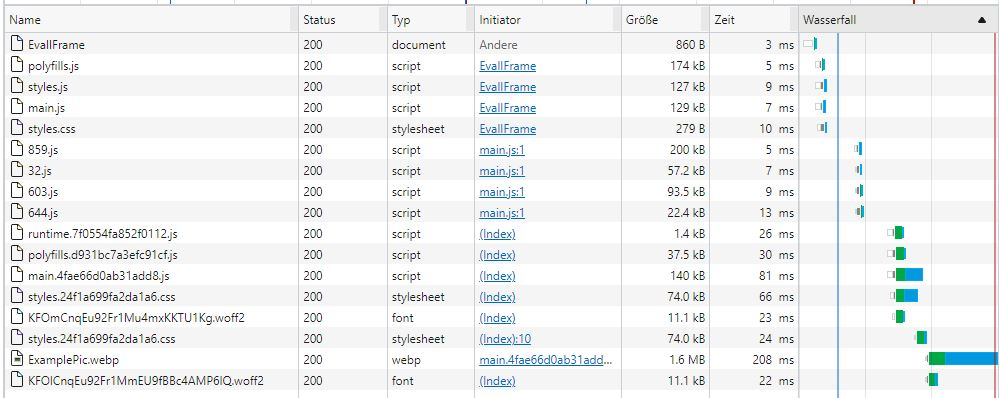
\includegraphics[width=1\textwidth]{img/appendix/Messung_IFrame}}\\ % Pfad
		\source{Eigene Darstellung} % Quelle
		\label{fig:MessungIFrame}
	\end{minipage}
\end{figure}

\newpage
\begin{figure}[hbt!]
	\centering
	\begin{minipage}[t]{1\textwidth}	
		\caption{Evaluierung Messung Web Component}
		\frame{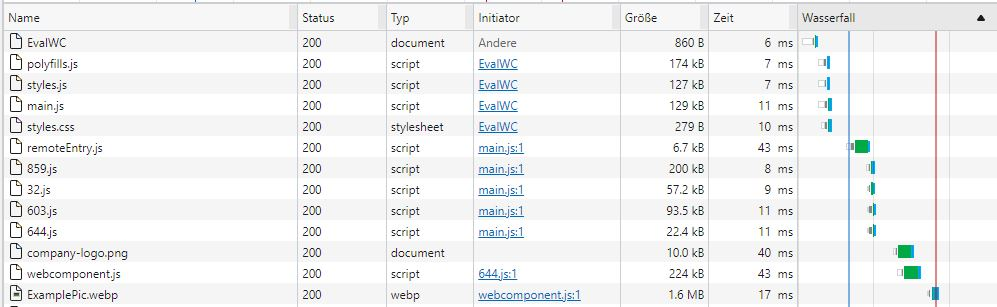
\includegraphics[width=1\textwidth]{img/appendix/Messung_WC}}\\ % Pfad
		\source{Eigene Darstellung} % Quelle
		\label{fig:MessungWebComponent}
	\end{minipage}
\end{figure}

\begin{figure}[hbt!]
	\centering
	\begin{minipage}[t]{1\textwidth}	
		\caption{Evaluierung Messung Module Federation}
		\frame{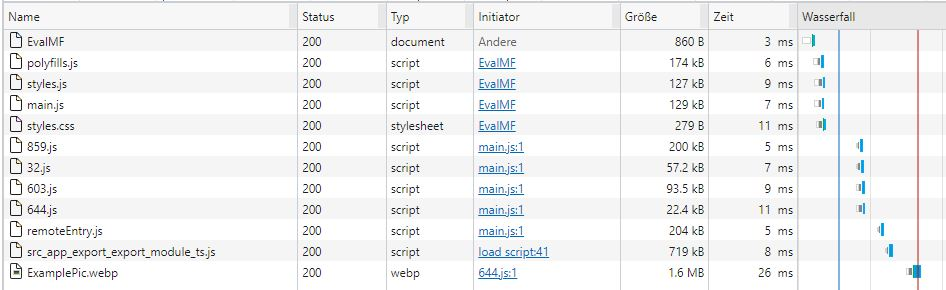
\includegraphics[width=1\textwidth]{img/appendix/Messung_MF}}\\ % Pfad
		\source{Eigene Darstellung} % Quelle
		\label{fig:MessungModuleFederation}
	\end{minipage}
\end{figure}

\begin{figure}[hbt!]
	\centering
	\begin{minipage}[t]{1\textwidth}	
		\caption{Evaluierung Messung Module Federation Web Components}
		\frame{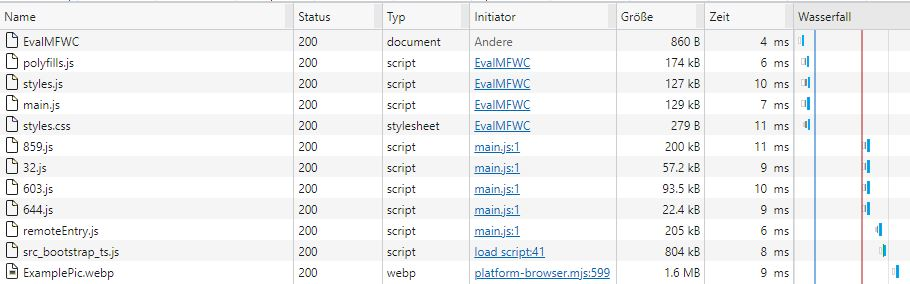
\includegraphics[width=1\textwidth]{img/appendix/Messung_MFWC}}\\ % Pfad
		\source{Eigene Darstellung} % Quelle
		\label{fig:MessungMFWC}
	\end{minipage}
\end{figure}

\newpage
\begin{figure}[hbt!]
	\centering
	\begin{minipage}[t]{0.65\textwidth}	
		\caption{HTML eines eingebundenen Iframes}
		\frame{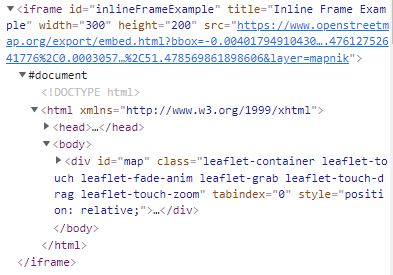
\includegraphics[width=1\textwidth]{img/appendix/IFrameHTML.JPG}}\\ % Pfad
		\source{Eigene Darstellung} % Quelle
		\label{fig:IFrameHTML}
	\end{minipage}
\end{figure}

\begin{figure}[hbt!]
	\centering
	\begin{minipage}[t]{0.6\textwidth}	
		\caption{Populärste Web Frameworks 2021}
		\frame{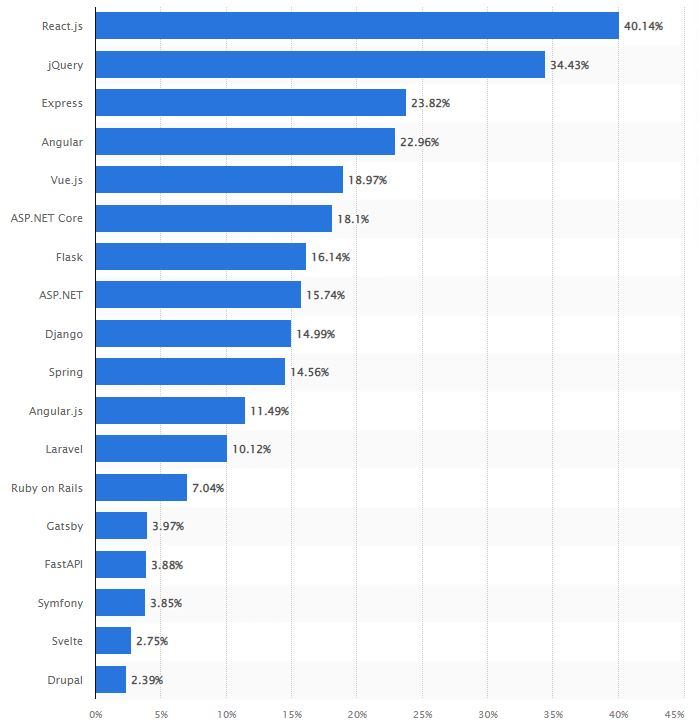
\includegraphics[width=1\textwidth]{img/appendix/FrontendFrammeworks.JPG}}\\ % Pfad
		\source{\cite[][]{Statista2022b}} % Quelle
		\label{fig:WebFrameworks}
	\end{minipage}
\end{figure}

\newpage
\begin{figure}[hbt!]
	\centering
	\begin{minipage}[t]{0.8\textwidth}	
		\caption{Marktanteile der führenden Browser}
		\frame{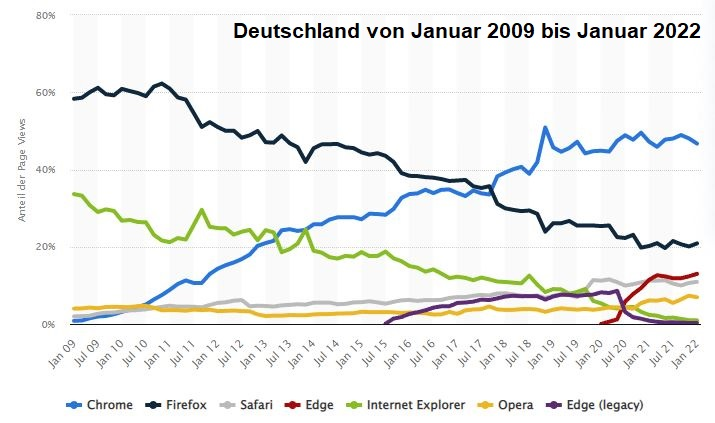
\includegraphics[width=1\textwidth]{img/appendix/StatistikBrowsernutzung.JPG}}\\ % Pfad
		\source{\cite[][]{Statista2022}} % Quelle
		\label{fig:StatistikBrowser}
	\end{minipage}
\end{figure}

\begin{figure}[hbt!]
	\centering
	\begin{minipage}[t]{0.8\textwidth}	
		\caption{Teilen von Daten bei Module Federation}
		\frame{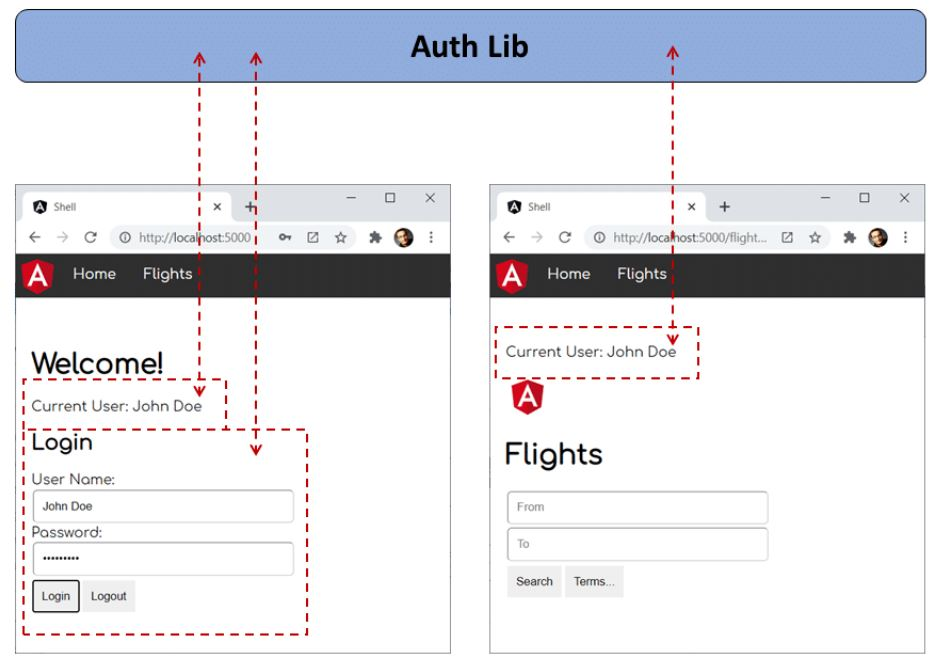
\includegraphics[width=1\textwidth]{img/appendix/ModuleFederationSharingData.JPG}}\\ % Pfad
		\source{\cite[][63]{Steyer2020}} % Quelle
		\label{fig:ModuleFShareData}
	\end{minipage}
\end{figure}

\newpage
\begin{figure}[hbt!]
	\centering
	\begin{minipage}[t]{1\textwidth}	
		\caption{Durchgeführte Messungen mit durchschnittlicher Datenmenge}
		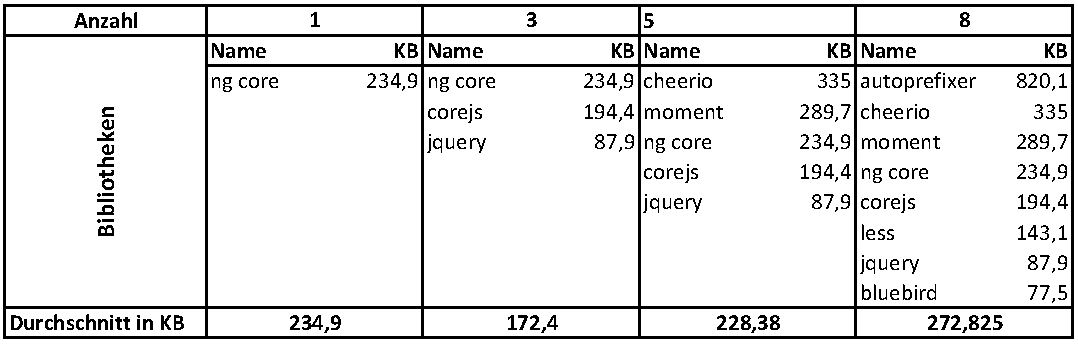
\includegraphics[width=1\textwidth]{img/appendix/DatasizeEval/GGBibliothekenMessungen.pdf}\\ % Pfad
		\source{Eigene Darstellung} % Quelle
		\label{fig:GGMessungBibs}
	\end{minipage}
\end{figure}

\begin{figure}[hbt!]
	\centering
	\begin{minipage}[t]{1\textwidth}	
		\caption{Doppelte Datenmenge durch zweifach eingebundenes Iframe}
		\frame{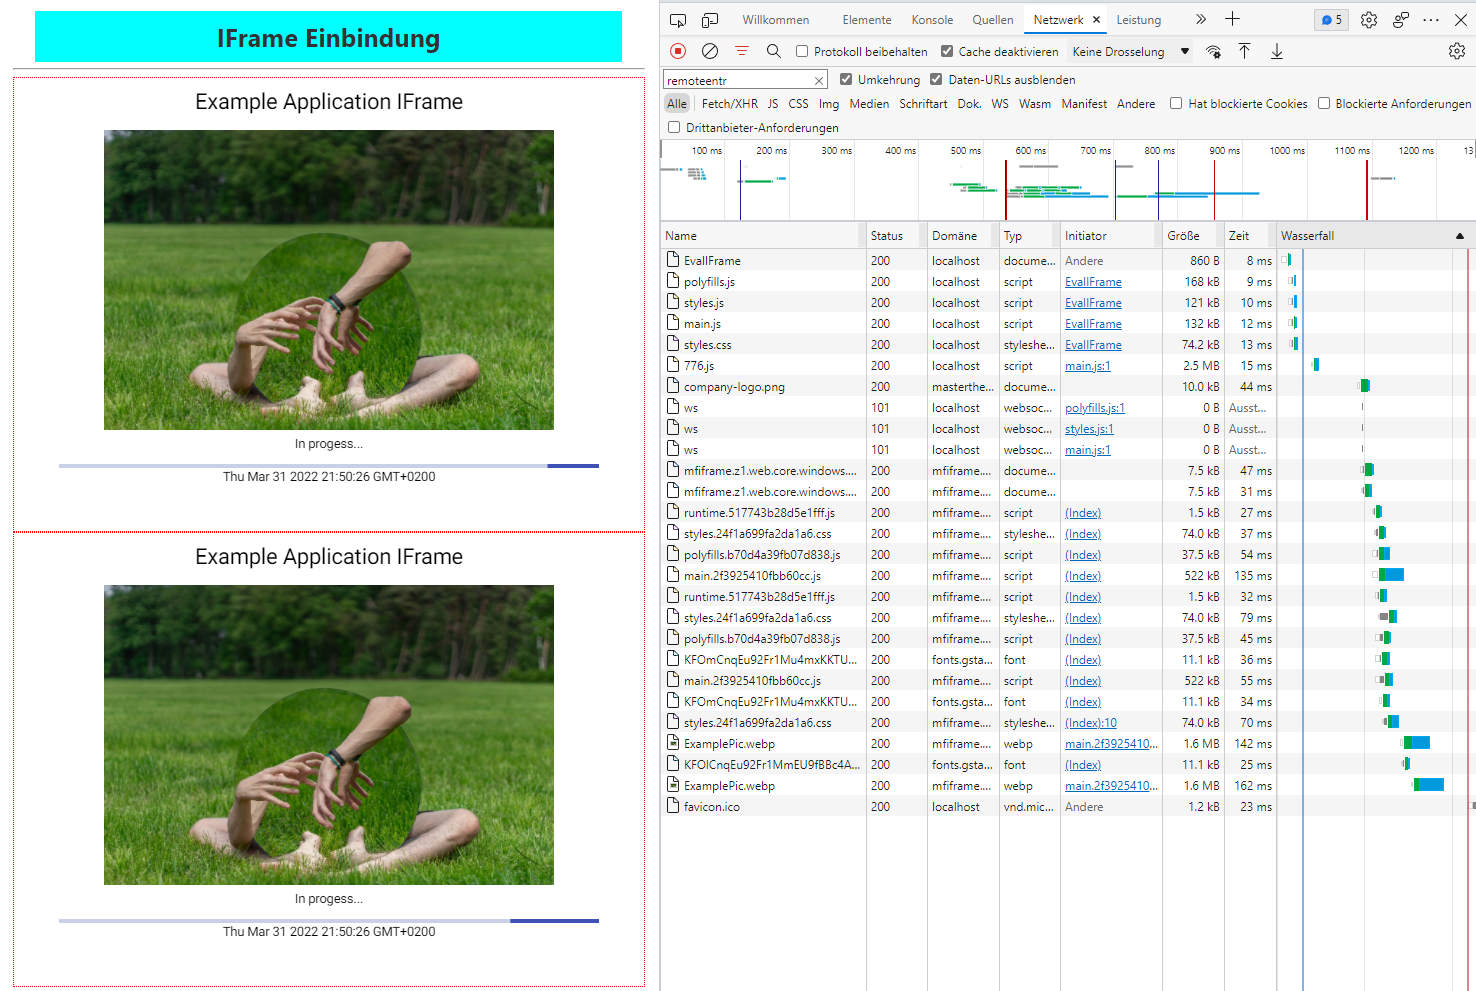
\includegraphics[width=1\textwidth]{img/appendix/Eval_Iframe_Skalierung}}\\ % Pfad
		\source{Eigene Darstellung} % Quelle
		\label{fig:EvalIframeSkalierbarkeit}
	\end{minipage}
\end{figure}

\newpage
\begin{figure}[hbt!]
	\centering
	\begin{minipage}[t]{0.5\textwidth}	
		\caption{Eingebundenes Iframe mit abgekapselten Stylings}
		\frame{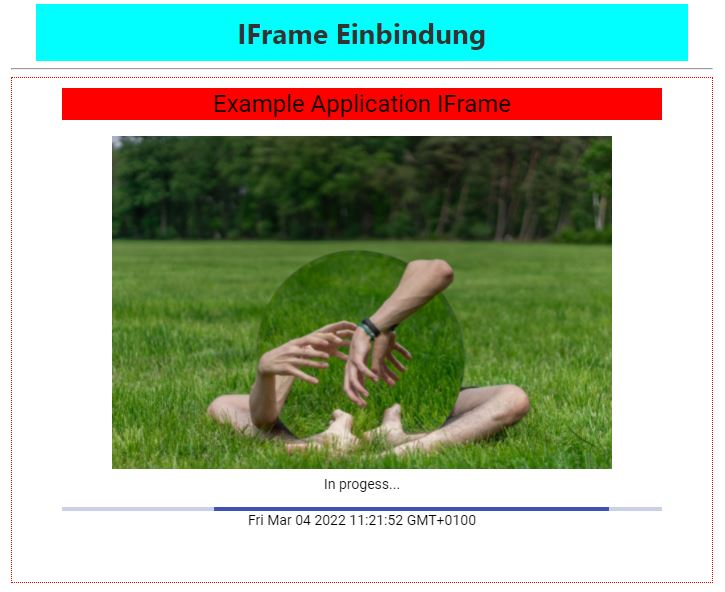
\includegraphics[width=1\textwidth]{img/appendix/Eval_Iframe_Beeinflussung.JPG}}\\ % Pfad
		\source{Eigene Darstellung} % Quelle
		\label{fig:EvalIframeBeeinflussung}
	\end{minipage}
\end{figure}

\begin{figure}[hbt!]
	\centering
	\begin{minipage}[t]{0.75\textwidth}	
		\caption{Sequenzdiagramm einer Zusammensetzung durch Nginx SSI}
		\frame{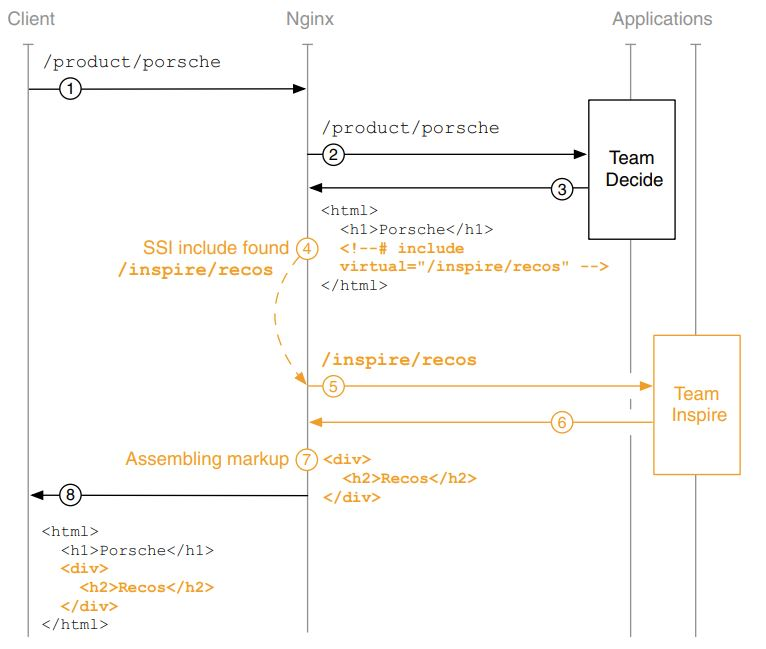
\includegraphics[width=1\textwidth]{img/appendix/SSCNginxSSI}}\\ % Pfad
		\source{\cite[][62]{Geers2020}} % Quelle
		\label{fig:SSCNginxSSI}
	\end{minipage}
\end{figure}

\newpage
\begin{figure}[hbt!]
	\centering
	\begin{minipage}[t]{1\textwidth}	
		\caption{Entscheidungsbaum Technologie Microfrontends}
		\frame{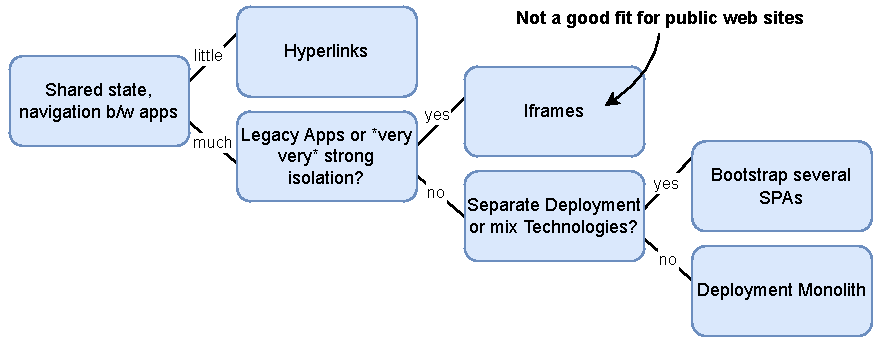
\includegraphics[width=1\textwidth]{img/appendix/EntscheidungsbaumArchitekturMF}}\\ % Pfad
		\source{\cite[Eigene Darstellung in Anlehnung an][]{Steyer2018}} % Quelle
		\label{fig:EntscheidungsbaumArchitekturMF}
	\end{minipage}
\end{figure}

\begin{figure}[hbt!]
	\centering
	\begin{minipage}[t]{0.7\textwidth}	
		\caption{Laden der Wetter Web Component}
		\frame{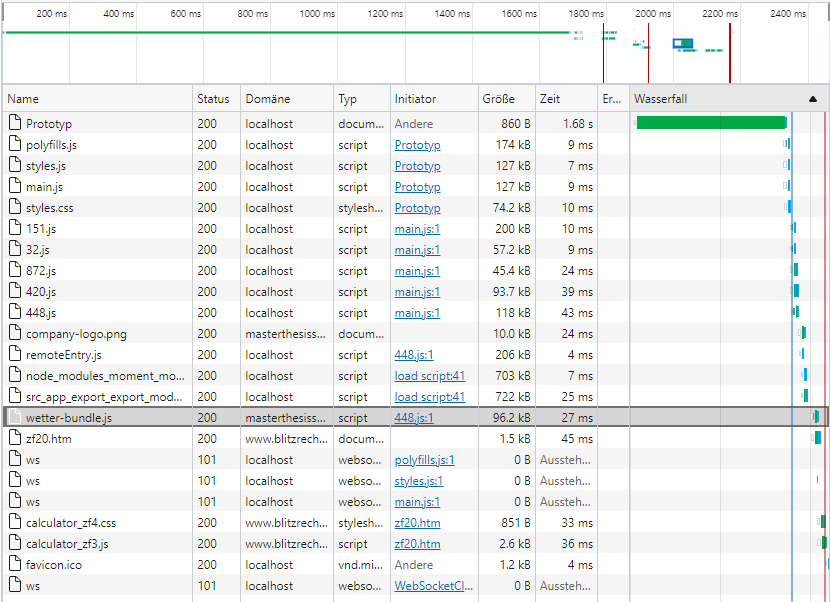
\includegraphics[width=1\textwidth]{img/appendix/PrototypEinmaligesLadenWC}}\\ % Pfad
		\source{Eigene Darstellung} % Quelle
		\label{fig:PrototypEinmaligesLadenWC}
	\end{minipage}
\end{figure}

\newpage
\begin{figure}[hbt!]
	\centering
	\begin{minipage}[t]{0.6\textwidth}	
		\caption{Event Emitter zum Übertragen von Daten}
		\frame{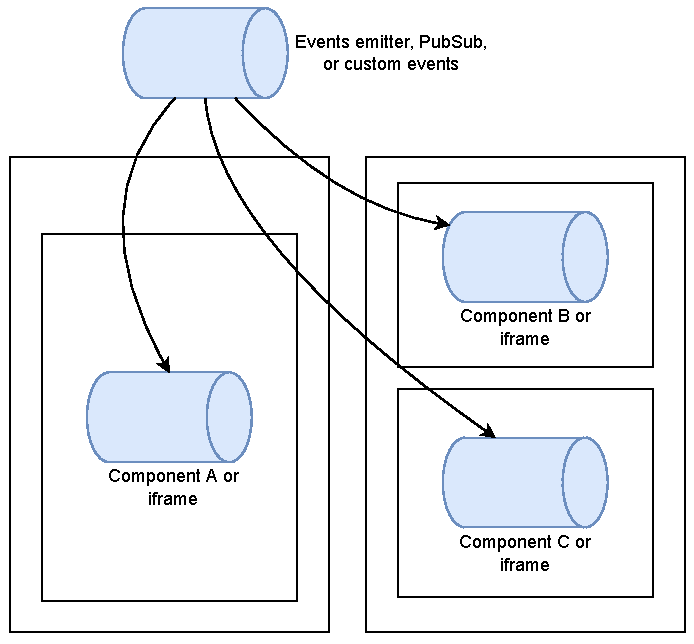
\includegraphics[width=1\textwidth]{img/appendix/MFSharingDataEventEmitter}}\\ % Pfad
		\source{\cite[Eigene Darstellung in Anlehnung an][33]{Mezzalira2021}} % Quelle
		\label{fig:MFSharingDataEventEmitter}
	\end{minipage}
\end{figure}

\begin{figure}[hbt!]
	\centering
	\begin{minipage}[t]{0.55\textwidth}	
		\caption{Web Storage zum Teilen von Daten}
		\frame{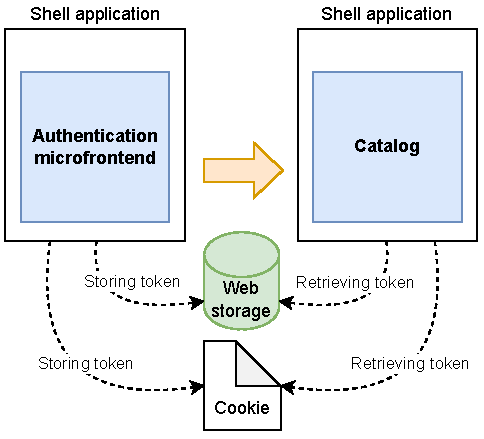
\includegraphics[width=1\textwidth]{img/appendix/MFSharingDataWebStorage}}\\ % Pfad
		\source{\cite[Eigene Darstellung in Anlehnung an][34]{Mezzalira2021}} % Quelle
		\label{fig:MFSharingDataWebStorage}
	\end{minipage}
\end{figure}

\newpage
\begin{figure}[hbt!]
	\centering
	\begin{minipage}[t]{0.65\textwidth}	
		\caption{Beispielhafte realisierte Lokalisierung bei Amazon}
		
\includegraphics[width=1\textwidth]{img/appendix/PortalshellLokalisierung.PNG}\\ % Pfad
		\source{Screenshot von Amazon} % Quelle
		\label{fig:PortalshellLokalisierung}
	\end{minipage}
\end{figure}

\begin{figure}[hbt!]
	\centering
	\begin{minipage}[t]{0.65\textwidth}	
		\caption{Zusammengefasste Präferenzmatrix mehrerer Teilnehmer}
		\includegraphics[width=1\textwidth]{img/Präferenzmatrix}\\ % Pfad
		\source{\cite[Eigene Darstellung in Anlehnung an][194]{Schierenbeck2016}} % Quelle
		\label{fig:PraeferenzmatrixBefuellt}
	\end{minipage}
\end{figure}

\newpage
\begin{figure}[hbt!]
	\centering
	\begin{minipage}[t]{0.65\textwidth}	
		\caption{Web Component in der eigenen Anwendung eingebunden}
		\frame{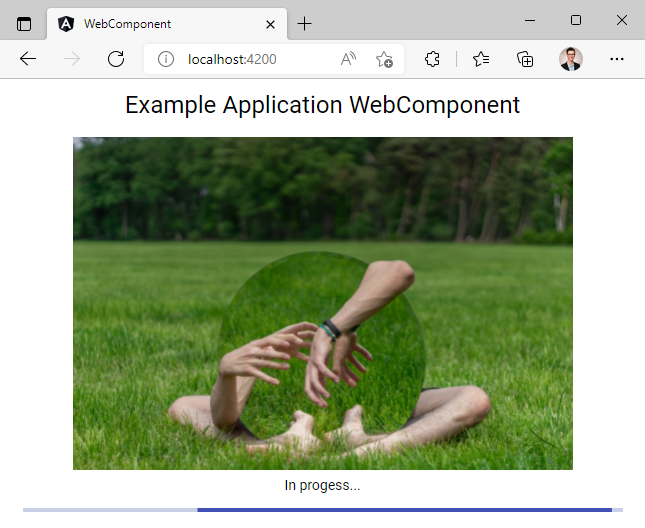
\includegraphics[width=1\textwidth]{img/appendix/WCSelbstEinbindung}}\\ % Pfad
		\source{Eigene Darstellung} % Quelle
		\label{fig:WCSelbstEinbindung}
	\end{minipage}
\end{figure}

\begin{figure}[hbt!]
	\centering
	\begin{minipage}[t]{0.65\textwidth}	
		\caption{Module Federation WC Beeinflussung Styles}
		\frame{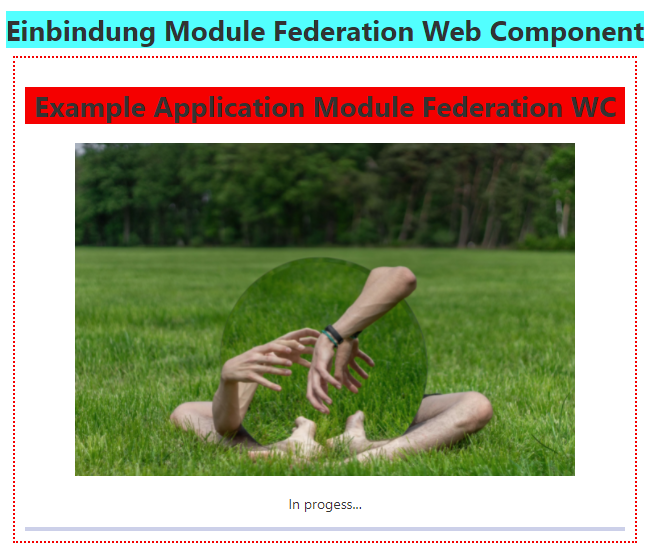
\includegraphics[width=1\textwidth]{img/appendix/Eval_MFWC_Beeinflussung.PNG}}\\ % Pfad
		\source{Eigene Darstellung} % Quelle
		\label{fig:EvalMFWCBeeinflussungStyles}
	\end{minipage}
\end{figure}

\newpage
\begin{figure}[hbt!]
	\centering
	\begin{minipage}[t]{0.65\textwidth}	
		\caption{Ladezeiten Module Federation WC bei 8 geteilten Bibliotheken}
		\frame{\includegraphics[width=1\textwidth]{img/appendix/DatasizeEval/MFWC_8.JPG}}\\ % Pfad
		\source{Eigene Darstellung} % Quelle
		\label{fig:EvalMFWCLadezeit}
	\end{minipage}
\end{figure}

\begin{figure}[hbt!]
	\centering
	\begin{minipage}[t]{0.7\textwidth}	
		\caption{Horizontaler Wissensaustausch in vertikalen Teams}
		\frame{\includegraphics[width=1\textwidth]{img/appendix/VertikaleTeamsWissensaustausch.PNG}}\\ % Pfad
		\source{\cite[][244]{Geers2020}} % Quelle
		\label{fig:VertikaleTeamsWissensaustausch}
	\end{minipage}
\end{figure}

\newpage
\begin{figure}[hbt!]
	\centering
	\begin{minipage}[t]{0.75\textwidth}	
		\caption{Schnittmengen von Frameworks bei Module Federation}
		\frame{\includegraphics[width=1\textwidth]{img/appendix/ModuleFederationWebComponentsDifferentFrameworkVersions}}\\ % Pfad
		\source{\cite[Eigene Darstellung in Anlehnung an][]{Steyer2021a}} % Quelle
		\label{fig:ModuleFederationSchnittmengenFrameworks}
	\end{minipage}
\end{figure}

\begin{figure}[hbt!]
	\centering
	\begin{minipage}[t]{0.65\textwidth}	
		\caption{Monolithisches Frontend vs. Microfrontend}
		\frame{\includegraphics[width=1\textwidth]{img/appendix/MonolithicMicrofrontend}}\\ % Pfad
		\source{Eigene Darstellung} % Quelle
		\label{fig:MonolithicMicrofrontend}
	\end{minipage}
\end{figure}

\newpage
\begin{figure}[hbt!]
	\centering
	\begin{minipage}[t]{1\textwidth}	
		\caption{Skalierung Web Component doppelte Einbindung}
		\frame{\includegraphics[width=1\textwidth]{img/appendix/Eval_WC_Skalierbarkeit}}\\ % Pfad
		\source{Eigene Darstellung} % Quelle
		\label{fig:EvalWCSkalierbarkeit}
	\end{minipage}
\end{figure}

\begin{figure}[hbt!]
	\centering
	\begin{minipage}[t]{1\textwidth}	
		\caption{Histogramm der Datenmenge von NPM-Paketen}
		\frame{\includegraphics[width=1\textwidth]{img/appendix/DatasizeEval/Histogramm}}\\ % Pfad
		\source{Eigene Darstellung} % Quelle
		\label{fig:HistogrammDatenmenge}
	\end{minipage}
\end{figure}

\newpage
\begin{figure}[hbt!]
	\centering
	\begin{minipage}[t]{1\textwidth}	
		\caption{Übersicht der Elemente der Portalapplikation mit Beispielen}
		\frame{\includegraphics[width=1\textwidth,page=5]{img/Beispielapplikation_Diagramm}}\\ % Pfad
		\source{Eigene Darstellung} % Quelle
		\label{fig:PortalapplikationElementeKonkret}
	\end{minipage}
\end{figure}

\begin{figure}[hbt!]
	\centering
	\begin{minipage}[t]{1\textwidth}	
		\caption{Laborsetup der Messungen}
		\includegraphics[width=1\textwidth]{img/appendix/Laborsetup}\\ % Pfad
		\source{Eigene Darstellung} % Quelle
		\label{fig:Laborsetup}
	\end{minipage}
\end{figure}

\newpage
\begin{figure}[hbt!]
	\centering
	\begin{minipage}[t]{0.7\textwidth}	
		\caption{Funktionsweise einer Portalapplikation}
		\frame{\includegraphics[width=1\textwidth]{img/appendix/AufgabenShell}}\\ % Pfad
		\source{\cite[][121]{Geers2020}} % Quelle
		\label{fig:AufgabenShell}
	\end{minipage}
\end{figure}

\begin{figure}[hbt!]
	\centering
	\begin{minipage}[t]{1\textwidth}	
		\caption{Microfrontend mit \textit{moment.js} geteilt durch Module Federation}
		\frame{\includegraphics[width=1\textwidth]{img/appendix/Messung_Moment_MF_Shared}}\\ % Pfad
		\source{Eigene Darstellung} % Quelle
		\label{fig:MomentMF}
	\end{minipage}
\end{figure}

\newpage
\anhang{Tabellen}\label{app:Tabellen}

\begin{table}[!hbt]
	\centering
	\begin{minipage}[t]{1\textwidth}
		\caption{Verwendete NPM-Pakete zum Vergleich der Datenmenge} % Überschrift
		\begin{tabularx}{\columnwidth}{| X | X |}
			\toprule
			\thead{\textbf{Name}} & \thead{\textbf{Datenmenge in KB (Stand 28.02.2022)}}\\
			\midrule
			autoprefixer & 820.1 \\
			cheerio & 335  \\
			moment & 289.7 \\
			@angular/core & 234,9 \\
			corejs & 194.4 \\
			less & 143.1 \\
			jquery & 87.9 \\
			bluebird & 77.5 \\			
			\midrule
			Durchschnitt & 272.8 \\
			\bottomrule
		\end{tabularx}
		\source{Eigene Darstellung}
		\label{tab:BibliothekenDatenmenge}
	\end{minipage}
\end{table}

\begin{table}[hbt]
	\centering
	\begin{minipage}[t]{\textwidth} % Breite, z.B. 1\textwidth		
		\caption{Übersicht der Rollen der prototypischen Portalshell} % Überschrift
		\begin{tabularx}{\columnwidth}{|c|c|X|}
			\toprule
			ID & Rollenname 		& Beschreibung \\
			\midrule
			1 & Anwender 				& Der Anwender darf die Portalapplikation benutzen, aber nichts konfigurieren. Er sieht die Dashboards seines Mandanten und kann die Microfrontendinstanzen in den Dashboards benutzen.\\
			\midrule
			2 & Administrator 			& Der Administrator darf die Portalapplikation sowie die Microfrontendinstanzen vollumfänglich nutzen. Er kann neue Benutzer registrieren und ihnen Rollen zuweisen. Ebenfalls sieht der Administrator eventuell mehr Inhalte in den Microfrontendinstanzen, sollte es dort Bereiche geben, die ausschließlich für Administratoren zugänglich sind. Der Administrator ist ebenfalls in der Lage Microfrontendinstanzen auf einem Dashboard zu platzieren und neu anzuordnen.\\
			\bottomrule
		\end{tabularx}
		\source{Eigene Darstellung}
		\label{tab:RollenPortalapplikation}
	\end{minipage}
\end{table}

\newpage
\anhang{Expertengespräche}\label{app:Expertengespräche}
\deffeat{Exp1}\\ \\
\underline{Expertengespräch mit Hanno Kortekamp}

Gesprächsprotokoll mit Hanno Kortekamp, Senior Software-Architekt bei einem großen deutschen IT-Dienstleister, mit mehr als 10 Jahren Berufserfahrung in Entwicklung und Betrieb von Portalapplikationen.\\
Durchgeführt am 20.12.2021 zu den Themen: Microfrontends, Portalapplikationen und Module Federation.

\textbf{Querschnittsaspekte von Portalapplikationen} 
\begin{compactitem}
   \item SDK für Formularelemente, Theme, UI und Styleguide
   \item Authentifizierung und Autorisierung
   \item Konfiguration
   \item Lokalisierung
   \item Navigation
   \item Mandantenfähigkeit
\end{compactitem}

\textbf{Messkriterien für Integration Microfrontends} 
\begin{compactitem}
	\item Übertragene Datenmenge
	\item Renderingzeit bis Darstellung
	\item Entwicklungsaufwand / Wartbarkeit
	\item Nähe am Standard
	\item Unterstützung verschiedener Frameworks
	\item (Browser)Kompatibilität
	\item Autonomie
	\item Unabhängigkeit der Entwicklerteams
	\item Lock-In Effekt	
\end{compactitem}

\textbf{Einsatz Module Federation im Projekt} 
\begin{compactitem}
	\item Nur Module Federation beschränkt Unabhängigkeit der Entwicklerteams
	\item Web Components in Kombination mit Module Federation mehr flexibel
\end{compactitem}

\newpage
\deffeat{Exp2}\\ \\
\underline{Expertengespräch im Rahmen der Nutzwertanalyse}

Diskussion im Rahmen der Nutzwertanalyse. Teilnehmerkreis bestehend aus:\\
Zwei Software-Architekten, zwei Software-Entwicklern und einem IT-Projektmanager.\\
Alle Teilnehmer haben bereits mehrjährige Erfahrungen mit Portalapplikationen und Microfrontends sammeln können.

Durchgeführt am 03.02.2022 zu den Themen: Vorstellung \& Diskussion gesammelter Kriterien sowie anschließende individuelle Durchführung der Paarvergleichsmethode. 

\textbf{Gesammelte Kriterien:}
\begin{compactitem}
	\item Datenmenge
	\item Renderingzeit
	\item Entwicklungsaufwand
	\item Wartbarkeit
	\item Nähe zum Standard
	\item Frameworks
	\item Kompatibilität
	\item Autonomie
	\item Unabhängige Entwicklerteams
	\item Lock-In Effekt
\end{compactitem}

Sowie Ergänzung des Kriteriums \textit{Interoperabilität}.

Anschließend individuelle Durchführung der Paarvergleichsmethode. Die einzelnen Paarvergleichsmatrixen sind dem beigefügten Anhang \ref{app:SonstigeDokumente} enthalten und in der \textit{Paarvergleichsmatrixen.zip} zu finden.

\newpage
\anhang{Sonstige Dokumente}\label{app:SonstigeDokumente}
Hinweis: Die sonstigen Dokumente sind nur in der beigefügten zip-Datei enthalten.\\

\begin{compactenum}
	\item Internetquellen
	\item Tabelle Nutzwertanalyse
	\item Tabellen Paarvergleichsmatrixen
	\item Tabelle Berechnung übertragene Datenmenge
	\item Messergebnisse geteilte Bibliotheken Web Components
	\item Quellcode Microfrontends
	\item Quellcode Portalshell inkl. StatistikApp
\end{compactenum}

%!TEX root = ../Thesis.tex
\section*{Quellenverzeichnis}
\addcontentsline{toc}{section}{Quellenverzeichnis}
\fancyhead[R]{Quellenverzeichnis}

\defbibheading{mono}{\subsection*{Monographien}}
\defbibheading{mag}{\subsection*{Aufsätze in Sammelbänden und Zeitschriften}}
\defbibheading{art}{\subsection*{Zeitungsartikel}}
\defbibheading{web}{\subsection*{Internetquellen}}
\defbibheading{leg}{\subsection*{Rechtsprechung}}
\defbibheading{comp}{\subsection*{Unternehmensunterlagen/Gesprächsnotizen}}

\setlength\bibitemsep{1.5\itemsep}
\setlength{\bibhang}{2em}

\renewcommand{\baselinestretch}{1.50}\normalsize

\begingroup
\sloppy

\printbibliography[heading=mono,keyword=mono]
\printbibliography[heading=web,keyword=web]

% Bei Bedarf einkommentieren: (erzeugt sonst Warnungen)
%\printbibliography[heading=mag,keyword=mag]
% \printbibliography[heading=art,keyword=art]
% \printbibliography[heading=leg,keyword=leg]
% \printbibliography[heading=comp,keyword=comp]

\endgroup


%%%%%%%%%%%%%%%%%%%%%%%%%%%%%%%%%%%%%%%%%%%%%%%%%%%%%%%%%%%%%%%%%%%%%%%

%!TEX root = ../Thesis.tex

\section*{Ehrenwörtliche Erklärung}
\addcontentsline{toc}{section}{Ehrenwörtliche Erklärung}
\fancyhead[R]{Ehrenwörtliche Erklärung}

Hiermit erkläre ich, dass ich die vorliegende \dokumententyp{} selbständig angefertigt habe. Es wurden nur die in der Arbeit ausdrücklich benannten Quellen und Hilfsmittel benutzt. Wörtlich oder sinngemäß übernommenes Gedankengut habe ich als solches kenntlich gemacht. Diese Arbeit hat in gleicher oder ähnlicher Form noch keiner Prüfungsbehörde vorgelegen.
\vspace{20mm}

\ort, \abgabedatum
\vspace{10mm}

\underline{\hspace{8cm}}\\\dokumentenautor
 
%%%%%%%%%%%%%%%%%%%%%%%%%%%%%%%%%%%%%%%%%%%%%%%%%%%%%%%%%%%%%%%%%%%%%%%

\end{document}